% Options for packages loaded elsewhere
\PassOptionsToPackage{unicode}{hyperref}
\PassOptionsToPackage{hyphens}{url}
\PassOptionsToPackage{dvipsnames,svgnames,x11names}{xcolor}
\documentclass[
  brazilian,
  11pt,
]{article}
\usepackage{xcolor}
\usepackage[margin=2.5cm]{geometry}
\usepackage{amsmath,amssymb}
\setcounter{secnumdepth}{-\maxdimen} % remove section numbering
\usepackage{iftex}
\ifPDFTeX
  \usepackage[T1]{fontenc}
  \usepackage[utf8]{inputenc}
  \usepackage{textcomp} % provide euro and other symbols
\else % if luatex or xetex
  \usepackage{unicode-math} % this also loads fontspec
  \defaultfontfeatures{Scale=MatchLowercase}
  \defaultfontfeatures[\rmfamily]{Ligatures=TeX,Scale=1}
\fi
\usepackage{lmodern}
\ifPDFTeX\else
  % xetex/luatex font selection
\fi
% Use upquote if available, for straight quotes in verbatim environments
\IfFileExists{upquote.sty}{\usepackage{upquote}}{}
\IfFileExists{microtype.sty}{% use microtype if available
  \usepackage[]{microtype}
  \UseMicrotypeSet[protrusion]{basicmath} % disable protrusion for tt fonts
}{}
\makeatletter
\@ifundefined{KOMAClassName}{% if non-KOMA class
  \IfFileExists{parskip.sty}{%
    \usepackage{parskip}
  }{% else
    \setlength{\parindent}{0pt}
    \setlength{\parskip}{6pt plus 2pt minus 1pt}}
}{% if KOMA class
  \KOMAoptions{parskip=half}}
\makeatother
\usepackage{longtable,booktabs,array}
\newcounter{none} % for unnumbered tables
\usepackage{calc} % for calculating minipage widths
% Correct order of tables after \paragraph or \subparagraph
\usepackage{etoolbox}
\makeatletter
\patchcmd\longtable{\par}{\if@noskipsec\mbox{}\fi\par}{}{}
\makeatother
% Allow footnotes in longtable head/foot
\IfFileExists{footnotehyper.sty}{\usepackage{footnotehyper}}{\usepackage{footnote}}
\makesavenoteenv{longtable}
\usepackage{graphicx}
\graphicspath{{docs/entregaveis/}{./}}
\makeatletter
\newsavebox\pandoc@box
\newcommand*\pandocbounded[1]{% scales image to fit in text height/width
  \sbox\pandoc@box{#1}%
  \Gscale@div\@tempa{\textheight}{\dimexpr\ht\pandoc@box+\dp\pandoc@box\relax}%
  \Gscale@div\@tempb{\linewidth}{\wd\pandoc@box}%
  \ifdim\@tempb\p@<\@tempa\p@\let\@tempa\@tempb\fi% select the smaller of both
  \ifdim\@tempa\p@<\p@\scalebox{\@tempa}{\usebox\pandoc@box}%
  \else\usebox{\pandoc@box}%
  \fi%
}
% Set default figure placement to htbp
\def\fps@figure{htbp}
\makeatother
\ifLuaTeX
\usepackage[bidi=basic,shorthands=off]{babel}
\else
\usepackage[bidi=default,shorthands=off]{babel}
\fi
\ifLuaTeX
  \usepackage{selnolig} % disable illegal ligatures
\fi
\setlength{\emergencystretch}{3em} % prevent overfull lines
\providecommand{\tightlist}{%
  \setlength{\itemsep}{0pt}\setlength{\parskip}{0pt}}
\usepackage{longtable,array}
\usepackage{newunicodechar}
\setlength{\emergencystretch}{3em}
\AtBeginDocument{\small}
\newunicodechar{→}{\ensuremath{\rightarrow}}
\newunicodechar{←}{\ensuremath{\leftarrow}}
\newunicodechar{↑}{\ensuremath{\uparrow}}
\newunicodechar{↓}{\ensuremath{\downarrow}}
\newunicodechar{χ}{\ensuremath{\chi}}
\newunicodechar{Δ}{\ensuremath{\Delta}}
\newunicodechar{σ}{\ensuremath{\sigma}}
\newunicodechar{≈}{\ensuremath{\approx}}
\newunicodechar{≤}{\ensuremath{\leq}}
\newunicodechar{≥}{\ensuremath{\geq}}
\newunicodechar{≫}{\ensuremath{\gg}}
\newunicodechar{∈}{\ensuremath{\in}}
\newunicodechar{−}{\ensuremath{-}}
\newunicodechar{‖}{\ensuremath{\Vert}}
\newunicodechar{⁻}{\ensuremath{^{-}}}
\newunicodechar{ᶻ}{\ensuremath{^{z}}}
\usepackage{bookmark}
\IfFileExists{xurl.sty}{\usepackage{xurl}}{} % add URL line breaks if available
\urlstyle{same}
\hypersetup{
  pdftitle={OLIMPO --- Fake News AI},
  pdfauthor={Equipe Olimpo --- PUC-Campinas e Instituto de Pesquisas ELDORADO},
  pdflang={pt-BR},
  colorlinks=true,
  linkcolor={Maroon},
  filecolor={Maroon},
  citecolor={Blue},
  urlcolor={Blue},
  pdfcreator={LaTeX via pandoc}}

\title{OLIMPO --- Fake News AI}
\usepackage{etoolbox}
\makeatletter
\providecommand{\subtitle}[1]{% add subtitle to \maketitle
  \apptocmd{\@title}{\par {\large #1 \par}}{}{}
}
\makeatother
\subtitle{Documento técnico consolidado: projeto, metodologia, dados, modelos, resultados e MVP}
\author{Equipe Olimpo --- PUC-Campinas e Instituto de Pesquisas ELDORADO}
\date{}

\begin{document}
\maketitle

{
\setcounter{tocdepth}{3}
\tableofcontents
}
Parceria: PUC-Campinas + Instituto de Pesquisas ELDORADO · Repositório: \texttt{olimpo-fake-news-ai}
Estado de referência, em 06/10/2026: branch \texttt{dev} (web-app e aprendizado não supervisionado) e branch \texttt{feat/svm-metadados-spacy} (aprendizado supervisionado e pipeline de produção \texttt{modelo\_olimpo.py}).

\begin{quote}
\textbf{Como ler este documento.} A ordem é a do raciocínio técnico (problema → método → dados → exploração → modelos → resultados → produto), e não a cronológica. Dois marcadores aparecem no texto:
\textbf{{[}NOTA{]}} registra uma correção ou uma decisão que mudou o que o texto anterior afirmava;
\textbf{{[}PENDENTE{]}} marca o que ainda não tem evidência no repositório e precisa ser executado ou confirmado antes da entrega. Todo marcador deve ser removido ou resolvido na versão final.
\end{quote}

\section{1. Projeto}\label{projeto}

\subsection{1.1 Situação encontrada}\label{situauxe7uxe3o-encontrada}

\paragraph{\texorpdfstring{\emph{O excesso de informação e a perda da confiabilidade}}{O excesso de informação e a perda da confiabilidade}}\label{o-excesso-de-informauxe7uxe3o-e-a-perda-da-confiabilidade}

Atualmente as plataformas digitais costumam priorizar conteúdos que geram cliques e engajamento rápido, muitas vezes deixando a precisão dos fatos em segundo plano. Com isso, a fronteira entre o jornalismo sério e a desinformação acabou se misturando, gerando uma crise global de confiança nas notícias.

\paragraph{\texorpdfstring{\emph{A queda do senso crítico e o efeito das "bolhas"}}{A queda do senso crítico e o efeito das "bolhas"}}\label{a-queda-do-senso-cruxedtico-e-o-efeito-das-bolhas}

Nesse cenário de consumo acelerado, o senso crítico das pessoas acaba enfraquecendo. A sobrecarga de notícias, somada aos algoritmos, nos coloca dentro de "bolhas" de conteúdo. Nelas, somos expostos quase exclusivamente a opiniões que confirmam o que já pensamos. Isso desestimula a checagem das fontes e nos torna mais vulneráveis a aceitar narrativas apelativas (ou falsas) como verdades absolutas, sem qualquer questionamento.

\paragraph{\texorpdfstring{\emph{O impacto na sociedade}}{O impacto na sociedade}}\label{o-impacto-na-sociedade}

Esse fenômeno não fica restrito à internet; os efeitos atingem o nosso dia a dia. A desinformação alimenta a polarização extrema e destrói a confiança nas instituições, na educação, na ciência e na própria democracia. Quando a sociedade perde a capacidade de separar o fato da ficção, tomamos decisões piores sobre assuntos vitais, como nossa saúde e nossos direitos, transformando uma falha tecnológica em uma verdadeira crise social.

\subsection{1.2 Solução proposta}\label{soluuxe7uxe3o-proposta}

Para combater o problema da desinformação na raiz, vamos desenvolver um site avaliador de notícias. Diferente das ferramentas tradicionais de checagem de fatos, que se limitam a carimbar um texto como "verdadeiro" ou "falso", nossa plataforma foi pensada para ser um ambiente interativo. O objetivo não é apenas classificar a informação inserida, mas reeducar o olhar do leitor e devolver a sua autonomia intelectual.

\paragraph{\texorpdfstring{\emph{Por que usaremos perguntas socráticas?}}{Por que usaremos perguntas socráticas?}}\label{por-que-usaremos-perguntas-socruxe1ticas}

Se o sistema apenas ditar que algo é mentira, um usuário pode simplesmente rejeitar a ferramenta por entrar em conflito com suas crenças. Para contornar essa barreira, escolhemos integrar o Método Socrático. Em vez de entregar um veredito impositivo, a plataforma estimula o pensamento crítico fazendo perguntas guiadas, como: "O termo "URGENTE" apareceu 10 vezes, isso é confiável?" ou "Existe uma referenciação da fonte?". Essa aprendizagem ativa ajuda o indivíduo a perceber as falhas de lógica por si mesmo, quebrando o viés de confirmação.

\subsubsection{Evolução do escopo}\label{evoluuxe7uxe3o-do-escopo}

O documento de concepção descreve um \textbf{avaliador individual de notícias} com perguntas socráticas. O produto em desenvolvimento no repositório evoluiu para uma \textbf{plataforma gamificada e colaborativa} (estilo Kahoot): jogadores em salas multiplayer ou solo recebem manchetes e votam entre \emph{Fake}, \emph{Fato real} e \emph{Tenho dúvida}; ao fim de cada rodada o sistema revela o gabarito e uma justificativa pedagógica. O componente de IA continua sendo o diferencial, pois é ele que fornece a classificação e a explicação usadas como feedback educativo. A seção 8 detalha o que já foi implementado.

\subsubsection{Princípio central e posicionamento}\label{princuxedpio-central-e-posicionamento}

A IA \textbf{não substitui o julgamento humano}. O produto deve estimular o pensamento crítico, apresentar indícios e deixar claras as limitações do modelo. Por isso a solução é posicionada como uma plataforma educacional que identifica padrões associados à confiabilidade de informações, e \textbf{não} como um "detector definitivo de fake news": o modelo trabalha com padrões aprendidos de um dataset e está sujeito a erros, vieses e mudanças de contexto (seção 7.3). Esse posicionamento é coerente com os resultados: a generalização fora do Fake.br é fraca, e a saída do modelo é apresentada como indício.

\subsection{1.3 Escopo e priorização (MoSCoW)}\label{escopo-e-priorizauxe7uxe3o-moscow}

Para viabilizar essa solução, estruturamos as prioridades de desenvolvimento da plataforma da seguinte maneira, utilizando a metodologia MoSCoW:

\textbf{Requisitos Essenciais (\emph{Must Have}):}

\begin{itemize}
\tightlist
\item
  \textbf{Plataforma web (Site):} O ambiente principal e acessível onde a aplicação funcionará.
\item
  \textbf{Modo de uso individual (Solo):} Foco inicial na jornada de aprendizagem de um único usuário.
\item
  \textbf{Input do usuário:} Área dedicada para que a pessoa insira diretamente a notícia ou afirmação que deseja avaliar.
\item
  \textbf{Sistema de semáforo:} Classificação visual e intuitiva utilizando \emph{red flags} (alertas de desinformação) e \emph{green flags} (indícios de confiabilidade) nas afirmações testadas.
\item
  \textbf{Método socrático:} O núcleo do sistema, responsável por devolver a análise em formato de questionamentos reflexivos.
\end{itemize}

\textbf{Requisitos Desejáveis (\emph{Should Have}):}

\begin{itemize}
\tightlist
\item
  \textbf{Marcação pelo usuário:} o próprio leitor será desafiado a destacar as palavras que considera como \emph{red flags} no texto.
\item
  \textbf{Gamificação:} Uso de mecânicas de jogos para tornar o processo de checagem mais engajador e recompensador.
\item
  \textbf{Dinâmicas coletivas:} Expansão para uso em grupo e análise de padrões de comportamento de múltiplos usuários.
\end{itemize}

\textbf{Requisitos Potenciais (\emph{Could Have}):}

\begin{itemize}
\tightlist
\item
  \textbf{Integração do Método SIFT:} Possibilidade de aliar a técnica SIFT (\emph{Stop;} \emph{Investigate the Source; Find Better Coverage; Trace Claims, Quotes, and Media to the Original Context}) às perguntas socráticas.
\item
  \textbf{Faixa etária e localidade dos usuários:} Durante o cadastro na plataforma, solicitaremos a data de nascimento e a localização do usuário. A finalidade dessa coleta é agrupar o público demograficamente para identificar possíveis padrões de comportamento no consumo de informações dentro de cada região e geração. Dessa forma, o sistema poderá analisar e validar métricas específicas cruzando esses dados. Será possível verificar, por exemplo, a hipótese de que 95\% dos jovens tendem a clicar mais em notícias com gatilhos de \emph{clickbait} (textos apelativos como "Urgente", "Veja" ou "Saiba mais"), ou avaliar se os usuários de uma cidade específica, como Campinas, interagem de maneira diferente e apresentam outros vieses de confirmação ao lerem notícias de impacto local.
\item
  \textbf{Tooltips Socráticos:} Exibição interativa de perguntas reflexivas geradas pela socratic-llm ao interagir com os trechos destacados, instigando o senso crítico do leitor sem exigir resposta.
\end{itemize}

\begin{quote}
\textbf{{[}NOTA{]}} Situação dos requisitos \emph{Must Have} em 06/10/2026, verificada no código: \textbf{plataforma web} --- implementada (Next.js); \textbf{input do usuário} --- implementado como extração de notícia a partir de URL (\texttt{/api/news/extract}); \textbf{semáforo} --- implementado como votação em três níveis (\emph{reliable / uncertain / unreliable}); \textbf{método socrático} --- \textbf{parcial}: a tela de jogo exibe três cartões socráticos \textbf{fixos} (fonte, tom emocional e evidência) antes da revelação do gabarito, mas as perguntas não são geradas pelo modelo nem por LLM; \textbf{modo solo} --- backend de salas pronto, interface em andamento. O modelo de ML \textbf{ainda não está integrado} ao sistema: o serviço de análise é um \emph{mock} por palavras-chave (seção 8.4).
\end{quote}

\subsection{1.4 Indicadores de desinformação (parâmetros)}\label{indicadores-de-desinformauxe7uxe3o-paruxe2metros}

Como a inteligência artificial não sabe instintivamente o que é verdade ou mentira, nossa finalidade foi fornecer a ela um conjunto claro de indicadores baseados no formato e no comportamento do texto (parâmetros). Ao invés de tentar checar cada fato isoladamente, ensinaremos o modelo a identificar a estrutura da desinformação (vícios de linguagem, sensacionalismo e falta de transparência).

Algumas informações serão mais relevantes devido à grande disparidade entre as comparações de dados entre informações falsas e verdadeiras. No \_paper Towards automatically filtering fake news in Portuguese\_encontramos dados como 36\% dos erros ortográficos para notícias falsas enquanto 3\% dos erros estavam presentes em texto verídicas. Outro ponto relevante é a variedade linguística usando sinônimos para detalhar o conteúdo, notícias falsas possuem 119 em média enquanto notícias verdadeiras possuem uma média de 494.

Isso garante que a solução seja rápida, escalável e capaz de justificar de forma lógica e transparente a análise de confiabilidade gerada para o usuário através da lógica de semáforo (\emph{red} e \emph{green flag}).

\paragraph{\texorpdfstring{\emph{Palavras 100\% em maiúsculo (Caixa Alta):}}{Palavras 100\% em maiúsculo (Caixa Alta):}}\label{palavras-100-em-maiuxfasculo-caixa-alta}

Na internet, escrever em maiúsculo equivale a gritar. O jornalismo profissional raramente usa esse recurso. Para o modelo, o excesso de palavras em CAIXA ALTA é um forte indicador de sensacionalismo, exagero e intenção de atrair cliques (\emph{clickbait}).

\paragraph{\texorpdfstring{\emph{Erros Ortográficos e gramaticais:}}{Erros Ortográficos e gramaticais:}}\label{erros-ortogruxe1ficos-e-gramaticais}

Veículos de comunicação reconhecidos possuem processo de revisão e edição do conteúdo, para que não haja uma publicação com erros. Consequentemente, o modelo efetuará uma avaliação no texto, entendendo se há erros frequentes, concordâncias mal colocadas, frases construídas incorretamente, geralmente tendem a ser padrões em notícias falsas.

\paragraph{\texorpdfstring{\emph{Verbos no imperativo:}}{Verbos no imperativo:}}\label{verbos-no-imperativo}

Expressões que enviesam os leitores, tais como "Compartilhe antes que apague", "Clique aqui agora", "Divulgue entre os familiares e amigos", tendem a forçar uma ação, que por muitas vezes são tendenciosas. Com isso, o modelo aprenderá a identificar o imperativo como uma tentativa de manipulação, onde o foco é a viralização, e não a informação em si.

\paragraph{\texorpdfstring{\emph{Emoções no texto e senso de urgência:}}{Emoções no texto e senso de urgência:}}\label{emouxe7uxf5es-no-texto-e-senso-de-urguxeancia}

A mentira viaja rápido porque mexe com nossos instintos. A desinformação usa o medo, a raiva ou a ansiedade para "desligar" o raciocínio lógico do leitor. Através da análise de sentimento, o modelo detecta gatilhos de urgência ("Alerta grave!", "Cuidado!") que tentam provocar reações impulsivas, e tendem a ser tendenciosas para o engajamento.

\paragraph{\texorpdfstring{\emph{Identificação do responsável (Autoria, Empresa):}}{Identificação do responsável (Autoria, Empresa):}}\label{identificauxe7uxe3o-do-responsuxe1vel-autoria-empresa}

A falta de um autor claro (um jornalista, uma agência de notícias ou uma empresa verificada) é um sintoma clássico de notícias falsas. O modelo procura pela autoria; se o texto não tem um "dono" para se responsabilizar pelo que foi dito, a confiabilidade cai. Alguns exemplos negativos: "relatado por alunos", "comprovado por especialistas". Exemplos positivos: "relatados por alunos da PUC Campinas", "comprovado por especialistas do instituto Eldorado".

\paragraph{\texorpdfstring{\emph{Fora ou Falta de Contexto:}}{Fora ou Falta de Contexto:}}\label{fora-ou-falta-de-contexto}

Uma das táticas mais perigosas da desinformação não é inventar uma mentira do zero, mas pegar um fato e tirá-lo de contexto (como usar um vídeo de 2019 dizendo que aconteceu ontem). O modelo avalia a estrutura do texto para checar se ele responde às perguntas básicas (quem, quando, onde), penalizando conteúdos vagos ou descontextualizados.

\subsection{1.5 Mapa de ideação}\label{mapa-de-ideauxe7uxe3o}

\pandocbounded{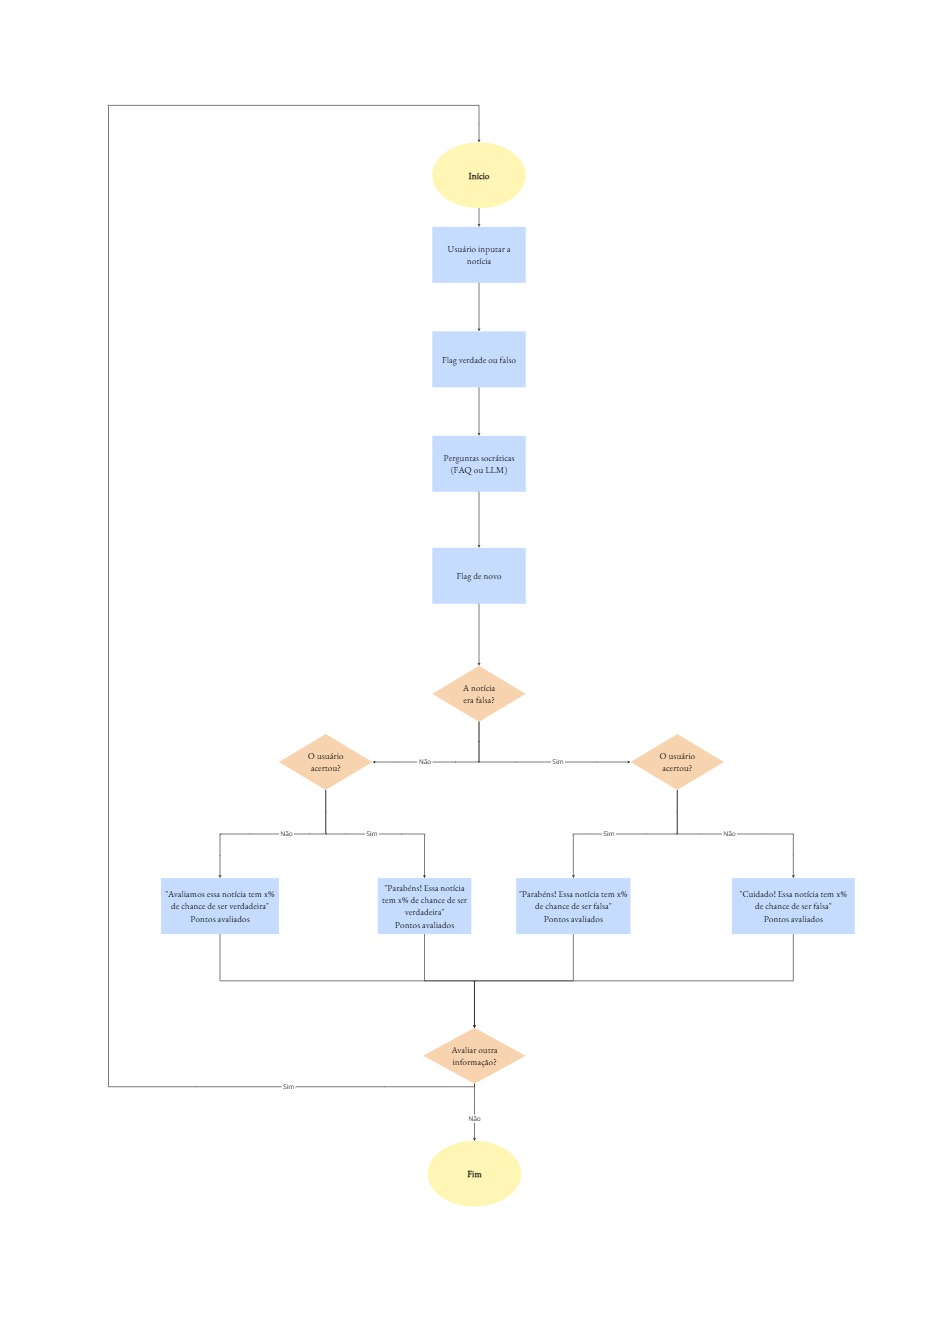
\includegraphics[keepaspectratio]{entregavel-final-img/fig01.jpg}}

\href{https://miro.com/app/board/uXjVHt4CciA=/}{Olimpo - Miro}

\section{2. Metodologias}\label{metodologias}

\subsection{2.1 Metodologia organizacional}\label{metodologia-organizacional}

Escolhemos a metodologia \emph{Crystal Clear} porque é eficiente para times pequenos e projetos rápidos. Essa metodologia também usa os principais conceitos da metodologia ágil, porém aplicados de um jeito mais flexível do que o Scrum ou o XP.

Além disso, o \emph{Crystal Clear} não define cargos rígidos, permitindo que cada pessoa participe de várias frentes do projeto. Isso se relaciona diretamente com o método CBL da residência e seus conceitos de \emph{group learning} e \emph{individual learning}: todos nos interessamos por todas as partes do projeto e queremos manter contato constante para sustentar o fluxo de aprendizado coletivo.

Também nos identificamos com as fases do \emph{Crystal Clear}:

\begin{itemize}
\tightlist
\item
  \emph{Reflection workshop:} Reunião periódica (geralmente ao final de cada incremento) para a equipe parar e analisar o que funcionou ou não no processo, equivalente à retrospectiva;
\item
  \emph{Iteration planning:} Reunião para definir as tarefas e funcionalidades do próximo ciclo de entrega;
\item
  \emph{Osmotic communication:} Mais do que uma reunião marcada, é a prática de manter o time no mesmo ambiente ou com canais abertos, para que as informações fluam de forma natural e contínua.
\end{itemize}

A partir disso, toda semana usaremos o que for necessário dessa metodologia, sempre seguindo esses conceitos, de forma a entregar o projeto e, ao mesmo tempo, permitir que cada integrante da equipe aprenda sobre as diferentes partes do sistema.

Para visualização, utilizaremos o quadro de tarefas no Jira, o qual organizaremos em Épicos, Histórias e Tarefas. Essa organização é uma das bases dos processos ágeis, dividindo os grandes objetivos em pequenas tarefas de curto prazo e menor esforço. Vamos usá-la para nos direcionar e conseguir dividir tarefas nas sprints, mantendo o grupo trabalhando de forma que o esforço seja equivalente e com prazos que fazem sentido.

\pandocbounded{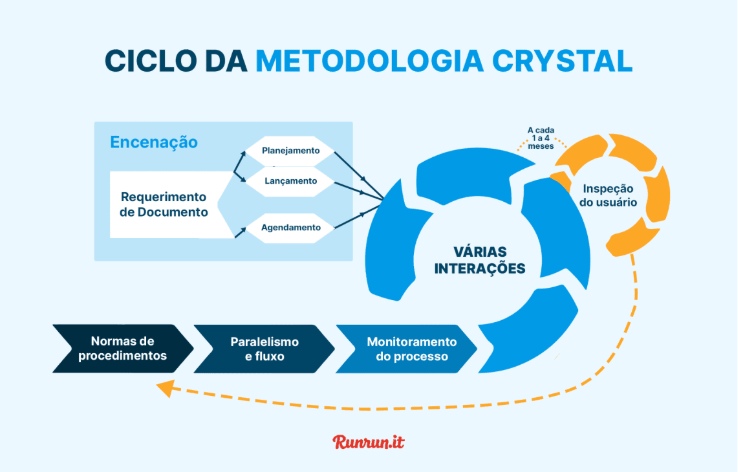
\includegraphics[keepaspectratio]{entregavel-final-img/fig02.png}}

\subsection{2.2 Frameworks}\label{frameworks}

\begin{itemize}
\tightlist
\item
  \textbf{RACI:} Responsável, Aprovador, Consultado e informado.\\
  Vamos usar essa matriz RACI para conseguirmos nos organizar previamente qual é a responsabilidade de cada um em uma determinada tarefa, ajudando a organização da equipe, já que o C\_rystal Clear\_ não demanda papéis fixos para cada pessoa durante o projeto.
\item
  \textbf{MoSCoW:} \emph{MUST HAVE, SHOULD HAVE, COULD HAVE, WON\textquotesingle T HAVE}
\end{itemize}

O MoSCoW vai ser utilizado para andar com o planejamento das sprints de desenvolvimento ao longo do projeto para definir o que vai ser mais necessário em cada parte do processo e o que deve ou não demandar esforço.

\begin{itemize}
\tightlist
\item
  \textbf{Planning Poker:} Definir média de esforço para cada uma das tarefas
\end{itemize}

Junto com o MoSCoW, o \emph{Planning poker} vai definir a média de esforço esperada para as tarefas em grupo e com isso conseguir separar tarefas por pessoa e tempo que vai demandar.

\subsection{2.3 Ferramentas}\label{ferramentas}

\subsubsection{\texorpdfstring{\textbf{Jira:} Plataforma para organização com quadro de tarefas}{Jira: Plataforma para organização com quadro de tarefas}}\label{jira-plataforma-para-organizauxe7uxe3o-com-quadro-de-tarefas}

Integrantes do grupo já tiveram contato com a plataforma então decidimos usá-la pela familiaridade, além de ter possibilidade de vincular com as branchs e PRs quando utilizarmos GitHub.

\subsubsection{\texorpdfstring{\textbf{GitHub:} Plataforma para os repositórios e versionamento do desenvolvimento do projeto}{GitHub: Plataforma para os repositórios e versionamento do desenvolvimento do projeto}}\label{github-plataforma-para-os-reposituxf3rios-e-versionamento-do-desenvolvimento-do-projeto}

\subsubsection{\texorpdfstring{\textbf{Google Colab:} Plataforma para o desenvolvimento de notebooks de maneira compartilhada}{Google Colab: Plataforma para o desenvolvimento de notebooks de maneira compartilhada}}\label{google-colab-plataforma-para-o-desenvolvimento-de-notebooks-de-maneira-compartilhada}

\subsection{2.4 Metodologia de modelagem de Machine Learning}\label{metodologia-de-modelagem-de-machine-learning}

\subsubsection{Separação e engenharia de dados}\label{separauxe7uxe3o-e-engenharia-de-dados}

\begin{itemize}
\tightlist
\item
  Os dados do Fake.br-Corpus (7.200 notícias, 3.600 por classe) são divididos em \textbf{80\% treino e 20\% teste}, de forma estratificada e com \texttt{random\_state=42}. O teste fica isolado de qualquer escolha de modelo, hiperparâmetro ou configuração.
\item
  Os textos passam por \textbf{normalização} e por \textbf{truncamento em 100 palavras} (detalhes na seção 5.2). A avaliação durante o desenvolvimento é feita por \textbf{validação cruzada estratificada, k=5, com embaralhamento (\texttt{random\_state=42})}.
\item
  A representação padrão é o \textbf{TF-IDF word+char}: unigramas e bigramas de palavras (\texttt{min\_df=2}) combinados com n-gramas de caracteres \texttt{char\_wb} de 3 a 5 (\texttt{min\_df=3}), ambos com \texttt{sublinear\_tf}.
\end{itemize}

\subsubsection{Modelo baseline}\label{modelo-baseline}

\begin{itemize}
\tightlist
\item
  A \textbf{Regressão Logística} é o baseline do projeto: fornece o patamar mínimo de desempenho, tem custo computacional baixo em espaços esparsos de alta dimensão e coeficientes diretamente interpretáveis.
\item
  Sob o pipeline atual, a LR com word+char obtém \textbf{F1-macro de 0,9182 ± 0,0136} na validação cruzada (C=1; \texttt{resultados\_C.csv}).
\end{itemize}

\subsubsection{Algoritmo de classificação escolhido}\label{algoritmo-de-classificauxe7uxe3o-escolhido}

\begin{itemize}
\tightlist
\item
  O \textbf{LinearSVC} (SVM linear) com word+char e C=1 é o classificador de referência: \textbf{F1-macro de 0,9295 ± 0,0099} na validação cruzada, contra 0,9182 da LR e 0,9285 do Random Forest com a configuração equivalente no protocolo anterior (seção 5.5).
\item
  A justificativa é estrutural: o TF-IDF gera \textasciitilde114 mil atributos para \textasciitilde5,7 mil documentos de treino (d ≫ N, \textasciitilde99,5\% de esparsidade), regime em que modelos lineares de margem máxima são eficientes e estáveis. Kernels não lineares não trouxeram ganho (seção 5.8).
\item
  O LinearSVC não produz probabilidades. No pipeline de produção (seção 5.11) ele é envolvido em \texttt{CalibratedClassifierCV} (sigmoide/Platt), que entrega \texttt{P(fake)} ao sistema.
\item
  \textbf{O modelo de produção é o M2 + χ² (10 mil) + SVD(500)}: word+char reduzido por χ² e SVD, somado ao bloco de metadados morfossintáticos spaCy, com LinearSVC calibrado (seções 5.6, 5.8 e 5.11). O word+char completo (B0) permanece como baseline de referência.
\end{itemize}

\subsubsection{Validação e prevenção de vazamentos}\label{validauxe7uxe3o-e-prevenuxe7uxe3o-de-vazamentos}

\begin{itemize}
\tightlist
\item
  Todos os estimadores e transformações (vetorizadores, imputação, padronização, seleção de atributos) ficam dentro de um \texttt{Pipeline} com \texttt{ColumnTransformer} do scikit-learn, ajustados somente com o treino de cada fold.
\item
  O desempenho no teste interno não deve ser lido como capacidade de generalização: o teste externo (seção 5.9) mostra queda de F1 de \textasciitilde0,93 para \textasciitilde0,61 fora do Fake.br.
\end{itemize}

\subsection{2.5 Governança de IA (AIPGF)}\label{governanuxe7a-de-ia-aipgf}

Definimos que utilizaríamos o AI Project Governance Framework (AIPGF), devido ao fato dele ser um modelo estruturado e pragmático focado na governança do uso de Inteligência Artificial em projetos. Onde o objetivo é garantir uma colaboração ética, eficiente e eficaz entre humanos e IA, mitigando riscos específicos, como vieses algorítmicos e questões de privacidade. Em vez de substituir metodologias de gestão, o AIPGF integra-se de forma fluida a abordagens já consolidadas, como Agile. Na prática, ele operacionaliza normas globais de alto nível, como a ISO/IEC 42001(ISO/IEC 42001 é a norma internacional para sistemas de gestão de IA), Lei Geral de Proteção de Dados (LGPD) e o \emph{National Institute of Standards and Technology} (NIST), aplicando suas exigências de conformidade diretamente à rotina dos projetos. Todo o framework é guiado por três princípios fundamentais: o centrismo humano, assegurando que a supervisão e a responsabilidade final sejam sempre das pessoas; a transparência, garantindo que o papel da IA seja explicável e auditável; e a adaptabilidade, permitindo que o modelo seja escalado e ajustado conforme o tamanho, a complexidade e o nível de risco de cada iniciativa.

\pandocbounded{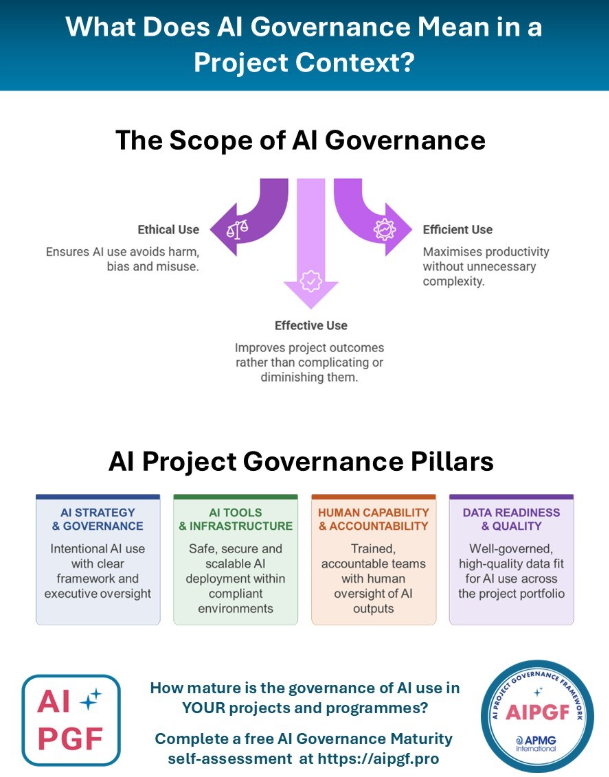
\includegraphics[keepaspectratio]{entregavel-final-img/fig03.png}}

\subsection{2.6 Mineração de dados (CRISP-DM)}\label{minerauxe7uxe3o-de-dados-crisp-dm}

O \emph{Cross-Industry Standard Process for Data Mining} (CRISP-DM) é uma metodologia estruturada e amplamente adotada para orientar o desenvolvimento de projetos de ciência de dados e inteligência artificial. Seu foco principal é fornecer um ciclo de vida padronizado e iterativo, garantindo que as soluções analíticas estejam estritamente alinhadas aos objetivos estratégicos da organização desde o início. O modelo organiza o projeto em seis fases contínuas e flexíveis: Entendimento do Negócio, Entendimento dos Dados, Preparação dos Dados, Modelagem, Avaliação e Implantação, devido a isso nós utilizaremos CRISP-DM.

\pandocbounded{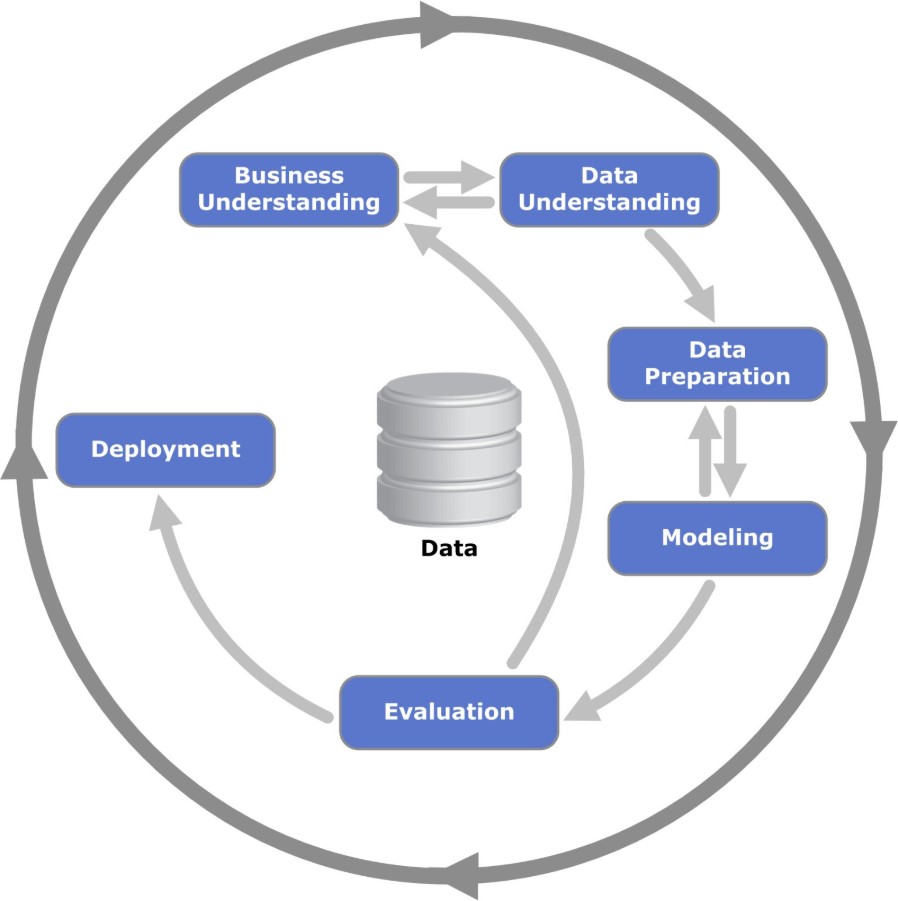
\includegraphics[keepaspectratio]{entregavel-final-img/fig04.png}}

\subsection{2.7 Metodologia de testes}\label{metodologia-de-testes}

\begin{itemize}
\tightlist
\item
  \textbf{Para testes de Dados:} Testes de Viés (Bias) e Equidade (Fairness)
\end{itemize}

Os testes de Viés e Equidade servem para manter o modelo de IA e \emph{Machine Learning} com decisões justas, éticas e não discriminatórias.

\begin{itemize}
\tightlist
\item
  \textbf{Para testes de código:} Testes Unitários, Teste de integração
\end{itemize}

Os testes unitários têm como intuito testar cada parte do sistema por sí só, esse tipo de teste demanda pouco tempo para fazer, porém, para cobrir o sistema inteiro a suíte de teste tem que ser muito extensa.

Já os testes de integração, focam em testar a integração entre testes unitários e serviços externos do projeto, demandam mais tempo que os unitários, mais custo, porém aparecem em menor quantidade.

Escolhemos focar nesses dois tipos de teste para desenvolver uma base forte sobre o sistema, em vínculo com os testes de dados e modelos. Na prática, o web-app também ganhou testes de ações simuladas ponta a ponta (\texttt{*.e2e.test.ts}, com logs \texttt{pino}) e um smoke test de interface com Playwright, executados no CI (seção 8).

\begin{quote}
\textbf{{[}NOTA{]}} Os testes de viés e equidade previstos para os dados não existiram como suíte própria. As análises que cumprem esse papel são: o controle de autoria (Cramér V = 0,960 entre autoria e rótulo), a dependência de marcadores temporais (seção 5.10) e a queda de desempenho no corpus externo (seção 5.9).
\end{quote}

\subsection{2.8 MLOps}\label{mlops}

\textbf{MLOps:} Disciplina para manter as boas práticas no desenvolvimento de modelos Machine Learning (ML)

Dentro do MLOps, temos 3 níveis separados em:

\subsubsection{\texorpdfstring{\textbf{MLOps}}{MLOps}}\label{mlops-1}

\paragraph{MLOps de nível 0}\label{mlops-de-nuxedvel-0}

Cada etapa é manual, incluindo preparação de dados, treinamento de \emph{Machine Learning} e performance e validação de modelos. Isso exige uma transição manual entre as etapas, e cada etapa é executada e gerenciada de maneira interativa. Os cientistas de dados normalmente entregam modelos treinados como artefatos que a equipe de engenharia implanta na infraestrutura da API.

O processo separa os cientistas de dados que criam o modelo e os engenheiros que o implantam, algo que em nosso caso, utilizando a metodologia Crystal não nos encaixou.

\begin{quote}
\textbf{{[}NOTA{]}} O estado real do projeto é o \textbf{nível 0}: preparação, treino e avaliação são feitos manualmente em notebooks, e o CI cobre apenas o web-app. A tentativa de versionar dados com DVC (PRs \#18--\#21) foi encerrada sem merge. O nível 1 permanece como meta, condicionada à integração do modelo ao sistema (seção 8.5).
\end{quote}

\paragraph{MLOps de nível 1 (meta do projeto)}\label{mlops-de-nuxedvel-1-meta-do-projeto}

O MLOps nível 1 visa treinar o modelo continuamente, automatizando o \emph{pipeline} de \emph{Machine Learning}, onde a maturidade de nível 1 tem as seguintes características:

Etapas rápidas do experimento de \emph{Machine Learning} que envolvem automação significativa

Treinamento contínuo do modelo em produção com dados atualizados como acionadores ativos do \emph{pipeline}

Implementação do mesmo \emph{pipeline} em ambientes de desenvolvimento, pré-produção e produção

\paragraph{MLOps de nível 2}\label{mlops-de-nuxedvel-2}

MLOps de nível 2, é adequado em situações em que há atualizações em modelos em minutos, onde é necessário retreinamento a cada hora ou diariamente e os reimplantam simultaneamente em milhares de servidores.

MLOps nível 2, necessita de:

Um orquestrador de pipeline de \emph{Machine Learning}

Um registro de modelos para rastrear vários modelos

Os três estágios a seguir se repetem em grande escala para vários \emph{pipelines} de \emph{Machine Learning} a fim de garantir a entrega contínua de modelos.

Se divide em 3 etapas:

Construir o \emph{pipeline}

Implantar o \emph{pipeline}

Fornecer o \emph{pipeline}

\pandocbounded{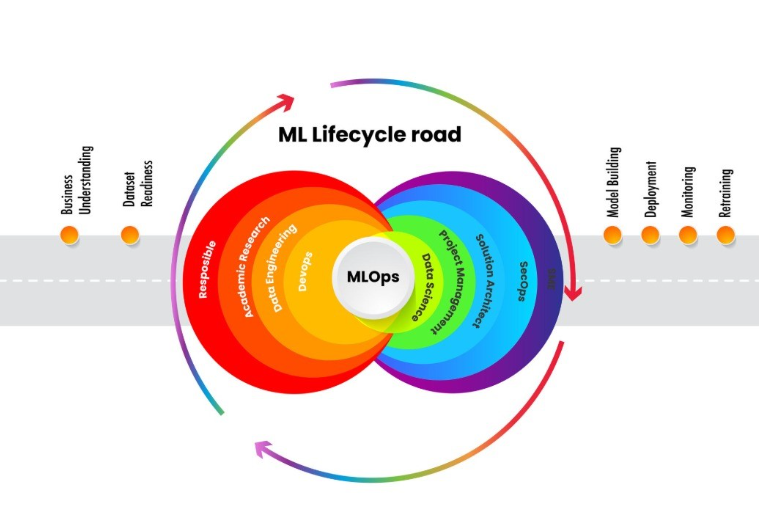
\includegraphics[keepaspectratio]{entregavel-final-img/fig05.png}}

\subsection{2.9 Metodologia de pesquisa}\label{metodologia-de-pesquisa}

\begin{itemize}
\tightlist
\item
  \textbf{Levantamento de campo:} Obtenção de dados no ambiente real afetado, principalmente por meio de entrevistas.
\item
  \textbf{Bibliográfica:} Pesquisa por meio da seleção e análise dos livros já publicados sobre o tema. Vai ser muito útil para fundamentar o problema.
\item
  \textbf{Netnografia:} É uma adaptação da etnografia tradicional, e é voltada para investigação de interações sociais, comportamentos e culturas no meio digital. Vamos usá-la para estudar como o público-alvo é afetado por informações de baixa confiabilidade e como pesquisam sobre, analisando a melhora ou piora do pensamento crítico na internet.
\end{itemize}

\subsection{2.10 Protocolo comum de comparação}\label{protocolo-comum-de-comparauxe7uxe3o}

O repositório define um protocolo comum para que métodos supervisionados e não supervisionados sejam comparáveis (\texttt{docs/machine-learning/comparacao-modelos/comparison-protocol.md}):

\begin{itemize}
\tightlist
\item
  Rótulos fixos (\texttt{0\ =\ True}, \texttt{1\ =\ Fake}); IDs, pastas de origem e labels servem para auditoria e nunca como feature.
\item
  Imputação, normalização, vocabulário TF-IDF e qualquer redução de dimensão são ajustados \textbf{somente no treino}.
\item
  Partição canônica com treino, validação e teste e \texttt{random\_state=42}, sem que um mesmo registro ou grupo (par temático, duplicata) apareça em mais de uma partição. Escolha de hiperparâmetros, limiares e regras usa a validação; o teste só é aberto depois de congelá-las.
\item
  Métricas principais: macro-F1 e balanced accuracy; também precisão e recall da classe Fake, taxa de falsos alertas em True, ROC-AUC e Average Precision. Scores de anomalia não são chamados de probabilidade de falsidade.
\item
  Clusterings que não atribuem notícias novas entram como análise exploratória, fora do ranking de classificação.
\end{itemize}

\begin{quote}
\textbf{{[}NOTA{]}} Os dois lados do projeto não seguem a mesma partição. O supervisionado usa divisão aleatória estratificada 80/20 por notícia; o não supervisionado usa partição por grupos (4.320 treino / 1.440 validação / 1.440 teste). O próprio protocolo reconhece que os números supervisionados antigos \textbf{não são comparação principal justa} e pede que os baselines sejam reexecutados na partição canônica. Essa reexecução ainda não foi feita (\textbf{{[}PENDENTE{]}}). Além disso, o supervisionado trunca em 100 palavras e o protocolo ainda cita 200.
\end{quote}

\section{3. Dataset}\label{dataset}

\subsection{3.1 Fake.br-Corpus}\label{fake.br-corpus}

O corpus utilizado é o \textbf{Fake.br-Corpus} (NILC/USP, em revisão fixa \texttt{780f5516c4ae070761632d98ac3368f3ded09d35}, validada por SHA-256 nos experimentos não supervisionados): \textbf{7.200 notícias em português, 3.600 falsas e 3.600 verdadeiras}, com texto completo, metadados e meta-informação linguística de cada uma. As falsas são, em geral, bem mais curtas (mediana de 157 palavras contra 918 nas verdadeiras), diferença que contamina qualquer atributo sensível a tamanho e motivou o truncamento descrito na seção 5.2.

\subsection{3.2 Seleção de campos}\label{seleuxe7uxe3o-de-campos}

Escolhemos esse dataset porque com ele teremos acesso a 7200 notícias já classificadas, sendo 3600 falsas e 3600 reais, além dos metadados de cada uma. Vamos fazer testes para achar a melhor combinação entre metadados e o texto da notícia, e a princípio já determinamos que alguns não serão necessários. Para maximizar a acurácia do modelo treinado com esse dataset tivemos que fazer alterações nos campos de metadados para trocar de números absolutos, nos campos de número de palavras, verbos, pronomes, substantivos, para taxa desses metadados a cada 100 palavras, a conta utilizada foi:\emph{numero\_absoluto}\_metadado \emph{/ numero\_total\_de\_palavras * 100}

\textbf{Campos que não vamos utilizar}

\textbf{Autor:} Campo onde cita o redator do texto. Não vamos utilizar

\pandocbounded{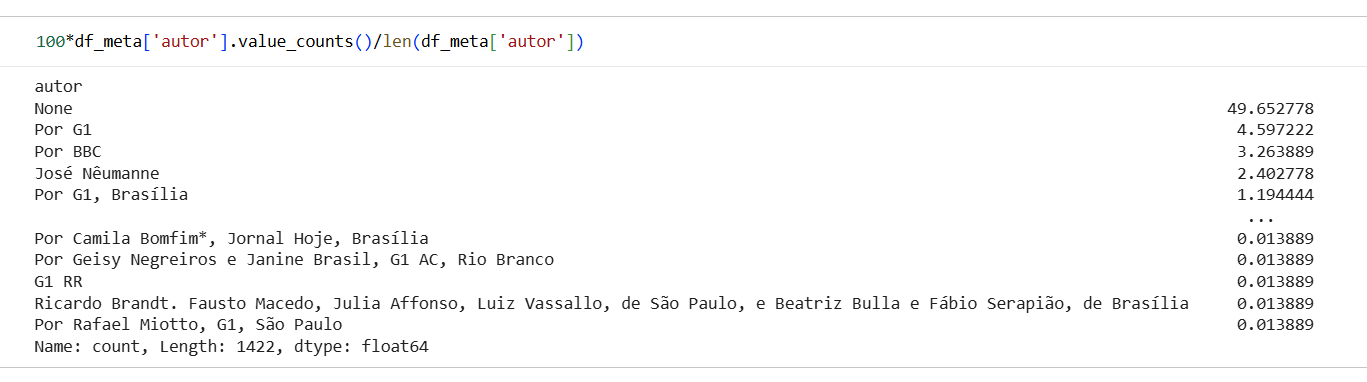
\includegraphics[keepaspectratio]{entregavel-final-img/fig06.png}}

\textbf{Categoria:} Campo para direcionar o grupo de notícias, mas não identificamos como um dado aplicável no nosso caso, visto que os verdadeiros e falsos possuem a mesma quantidade de cada categoria.

\pandocbounded{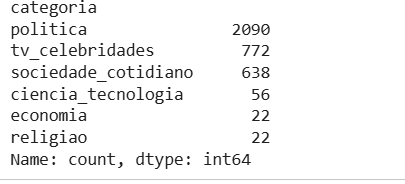
\includegraphics[keepaspectratio]{entregavel-final-img/fig07.png}}

\textbf{URL:} Campo com link da notícia. Não vamos utilizar pois a maioria dos links direciona para 3 sites específicos o que pode acabar criando um viés ruim para o treinamento do modelo.

\textbf{Label:} Responsável por identificar se a notícia é verdadeira ou não então está presente em todos as linhas

\textbf{Num\_links:} Número de links contidos no texto

\pandocbounded{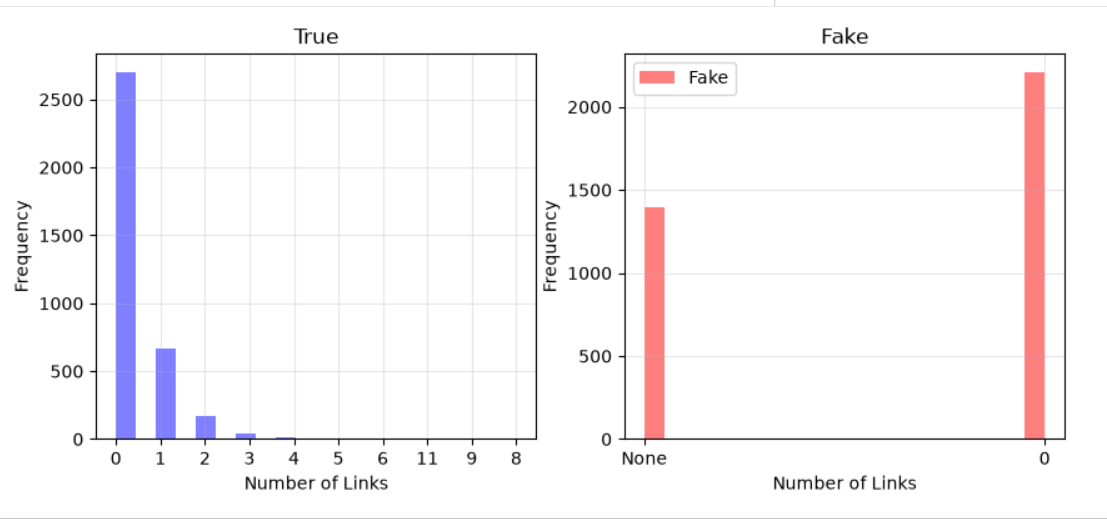
\includegraphics[keepaspectratio]{entregavel-final-img/fig08.png}}

\textbf{Campos para considerarmos}

\textbf{Texto:} Campo responsável por apresentar o corpo do texto (mudança feita apenas a truncagem dos dados para limitar o número de palavras evitando viés).

\textbf{Num\_maiusculas:} Conta o número de maiúsculas no texto. Em comparação o número de maiúsculas aparece muito mais considerando o tamanho do texto\pandocbounded{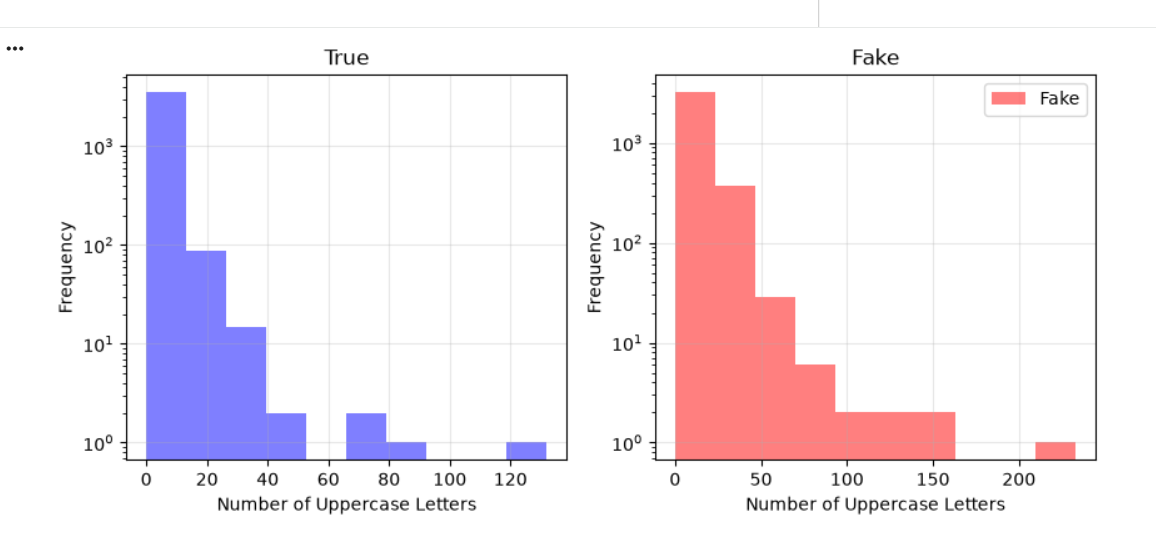
\includegraphics[keepaspectratio]{entregavel-final-img/fig09.png}}

\textbf{Campos ainda analisar}

Num\_verbos; num\_verbos; num\_verbos\_subj\_imp; num\_substantivos; num\_adjetivos; num\_adverbios; num\_verbos\_modais; num\_pron\_1\_2\_sing; num\_pron\_1\_plural;

num\_pronomes; Pausalidade; pct\_erros\_ortograficos; Emotividade; Diversidade.

\subsection{3.3 Corpus externo: FakeRecogna}\label{corpus-externo-fakerecogna}

Para medir generalização fora do Fake.br usa-se o \textbf{FakeRecogna} (HuggingFace \texttt{recogna-nlp/FakeRecogna}; 11.903 registros, 5.951 por classe). Como a coluna \texttt{Noticia} vem lematizada e sem stopwords, e boa parte dos textos "fake" são checagens que desmentem boatos, o teste externo usa \textbf{somente títulos}: os 2.484 títulos falsos do domínio \texttt{boatos.org} (sem a tag \texttt{\#boato}) e a mesma quantidade de títulos reais amostrados (\texttt{random\_state=42}), normalizados pela mesma função do \texttt{01\_Data\_Prep}. A mediana é de \textbf{13 palavras por título}, contra textos de até 100 palavras no treino: o teste mede, portanto, generalização de \textbf{domínio e de formato} ao mesmo tempo.

\subsection{3.4 Extração morfossintática própria (spaCy)}\label{extrauxe7uxe3o-morfossintuxe1tica-pruxf3pria-spacy}

Além dos metadados que acompanham o corpus (etiquetados pelo NILC sobre o texto completo), o projeto extrai seus próprios atributos por notícia com o spaCy (\texttt{pt\_core\_news\_sm}, módulo \texttt{metadados\_spacy.py}), sobre o mesmo texto normalizado e truncado que o TF-IDF vê. É a única fonte de metadados aplicável a notícias novas e ao FakeRecogna, que não possuem os metadados do corpus (resultados na seção 5.6).

\section{4. Análise exploratória de dados (EDA)}\label{anuxe1lise-exploratuxf3ria-de-dados-eda}

\subsection{4.1 Introdução}\label{introduuxe7uxe3o}

A análise exploratória de dados consiste em explorar, resumir e visualizar os dados através de uma série de etapas. Com essas etapas buscamos entender a estrutura, testar nossas suposições, identificar anomalias e encontrar padrões e relações entre \emph{features}. A análise exploratória de dados tem algumas variações e cada uma possui objetivos claros a atingir, sendo elas: a análise univariada, que tem o objetivo de entender a distribuição e variação de uma única \emph{feature;} bivariada, que serve para estudar o relacionamento entre duas variáveis; e a análise multivariada, que foca nas interações entre múltiplas variáveis. Neste documento, descreveremos quais análises foram realizadas e as informações obtidas.

\textbf{Etapas da análise exploratória de dados (EDA)}

\begin{enumerate}
\def\labelenumi{\arabic{enumi}.}
\tightlist
\item
  \textbf{Entender o objetivo e os dados}
\end{enumerate}

\begin{itemize}
\tightlist
\item
  O objetivo é treinar um algoritmo de classificação para determinar se uma notícia é verdadeira ou falsa, para nosso projeto.
\item
  Os tipos de dados no dataset encontrado foram Texto, Números (float e inteiros).
\end{itemize}

\begin{enumerate}
\def\labelenumi{\arabic{enumi}.}
\tightlist
\item
  \textbf{Importar e inspecionar}
\end{enumerate}

Nessa etapa importamos o dataset escolhido (Fake.br corpus) do github para o notebook (.ipynb) e transformamos os arquivos de texto em Data Frames do pandas. Com o intuito de facilitar a exploração, análise e manipulação de dados. Em resumo, no notebook, seguimos os passos de LOAD (carregamento dos dados no ambiente), CHECK (Avaliar os dados), IDENTIFY MISSING (Encontrar valores faltantes), VERIFY DATA TYPE (Verificar os tipos de dados) e FIND ERRORS AND INVALID VALUES (Encontrar erros e valores inválidos no meio do dataset).

\begin{enumerate}
\def\labelenumi{\arabic{enumi}.}
\tightlist
\item
  \textbf{Lidar com dados faltantes ou inválidos}
\end{enumerate}

Para lidarmos com mais certeza, primeiramente precisamos entender o porquê de os dados estarem faltantes ou inválidos, e percebemos que na maioria das vezes era em relação com a fonte, autor.

Após isso partimos para a etapa de remover ou preencher as células destacadas, e nos campos de metadados numéricos, que estavam com o tipo None, preenchemos com 0, já nos campos de fonte e autor, como tinham alta quantidade de valores vazios ou inválidos, decidimos cortar essas features do dataset.

Com isso, o impacto foi de um dataset padronizado com features do mesmo tipo e preenchidas com valores válidos e sem as features que deixariam o modelo desbalanceado.

\begin{enumerate}
\def\labelenumi{\arabic{enumi}.}
\tightlist
\item
  \textbf{Exploração das características dos Dados}
\end{enumerate}

Essa etapa consistiu em entender a distribuição dos dados, para qual utilizamos o boxplot, barcharts, histograms, no ambiente do colab, a tendencia central dos dados a partir do boxplot, a viabilidade do dado,a forma de distribuição e encontrar os outliers e anomalias. A etapa consistiu no tipo de EDA Univariada.

Juntamente com as análises de gráficos, também testamos treinar o modelo de regressão logística com diferentes features para explorar melhor e como a feature afeta no modelo.

\begin{enumerate}
\def\labelenumi{\arabic{enumi}.}
\tightlist
\item
  \textbf{Executar transformação nos dados}
\end{enumerate}

Após entender as características, transformar os dados para melhor atender nossa necessidade foi muito mais simples, na exploração havíamos nos alertado com o tamanho do texto, que enviesou o modelo a colocar extrema importância nisso, por isso cortamos os textos (inicialmente em 200 palavras; ver seção 5.2, em que o corte passou a 100 e foi acompanhado de normalização).

No entanto, os campos de metadados com números absolutos por texto por serem muito relativos ao tamanho do texto, isso também se relacionava com o quanto a notícia era falsa ou verdadeira, de forma que para o modelo, nos testes, era só uma notícia falsa ter maiores números absolutos para ser considerada como verdadeira e o modelo errar por isso. Por esse motivo decidimos transformar as features com valores absoluto relativos ao tamanho da notícia em taxas a cada 100 palavras, com a fórmula:

`numero\_absoluto / numero\_palavras * 100`.

Não precisamos usar o label encoding, já que o label estava como binário (0 é notícia verdadeira e 1 é notícia falsa).

Além disso não criamos features novas, estava nos planos adicionar a feature binária se tem autor ou não, porém, através da exploração, percebemos que o valor estava faltando em grande parte das notícias falsas, o que poderia enviesar o modelo.

Durante o processo de transformação, executamos diversos testes no modelo de regressão logística para conferir em tempo real o quanto a mudança fazia efeito, tanto para efeitos que melhoravam, tanto os que pioraram.

\begin{enumerate}
\def\labelenumi{\arabic{enumi}.}
\tightlist
\item
  \textbf{Visualizar a Relação dos dados}
\end{enumerate}

Nosso objetivo nessa etapa foi de descobrir e entender padrões, tendências e relações entre campos, que entra no tipo de EDA Bivariada e Multivariada. Para atingir melhores resultados, usamos gráficos de barra, histogramas, gráficos de dispersão como o pairplot e matriz de correlação, junto com heatmap para facilitar a visualização da matriz.

Com isso, percebemos que havia relações inesperadas entre os dados, como a taxa de maiúsculas ser mais presente em notícias com o label 1(falsas) a diversidade (número de palavras diferentes dividido pelo número de palavras) estar fortemente e diretamente relacionado com notícias com o label 0, (verdadeiras).

A visualização da relação entre dos dados foi ainda mais presente em conjunto com o modelo de regressão logística, que indicava o tamanho da relação ao omitir dados, incluir ou tratar o dado de forma diferente.

\begin{enumerate}
\def\labelenumi{\arabic{enumi}.}
\tightlist
\item
  \textbf{Lidar com Outliers}
\end{enumerate}

Para os Outliers, utilizamos principalmente o boxplot para identificá-los, no entanto, não executamos nenhuma ação de capping ou transformação nesses dados, já que durante as nossas pesquisas o que achamos foi que só outliers são excluídos apenas quando devidamente entendidos e incorretos.

\begin{enumerate}
\def\labelenumi{\arabic{enumi}.}
\tightlist
\item
  \textbf{Comunicar resultados}
\end{enumerate}

Estamos comunicando os resultados por meio desse documento sobre a nossa análise exploratória de dados com foco no dataset escolhido do Fake.br Corpus, nossos resultados até agora foi um treinamento do modelo de regressão logística de 92\% de acurácia com apenas o texto cortado em 200 palavras e tratado pelo método TF-IDF, e 95\% de acurácia com o texto (tratado pelo TF-IDF) junto com os metadados da notícia.

Treinamos um modelo não supervisionado também, porém apontou piores resultados do que o modelo supervisionado.

\begin{quote}
\textbf{{[}NOTA{]}} Os resultados citados na etapa "Comunicar resultados" (92\% de acurácia só com texto e 95\% com metadados) são das primeiras rodadas, com corte em 200 palavras e sem normalização, na Regressão Logística. Em rodadas posteriores os metadados pioraram a LR (−2,4 pontos de F1 em word+meta, protocolo anterior), o que levou a não adotá-los como bloco principal; a evidência no pipeline atual é conflitante (seção 5.6).
\end{quote}

\begin{quote}
\textbf{{[}PENDENTE{]}} Na etapa "Visualizar a relação dos dados", o texto afirma que a diversidade se associa às notícias \textbf{verdadeiras}, enquanto o boxplot, a correlação com o rótulo (0,8) e o FP-Growth (diversidade baixa → 61,6\% Fake) apontam o oposto. Uma hipótese a verificar é artefato de tamanho: a razão tipos/tokens decresce com o comprimento e as falsas são \textasciitilde6× mais curtas. Vale recomputar a correlação sobre os textos já truncados (\texttt{diversidade\_relativa}, MATTR de janela 100) e unificar a leitura.
\end{quote}

\subsection{4.2 Correlação entre variáveis}\label{correlauxe7uxe3o-entre-variuxe1veis}

A fim de compreender quais \emph{features} possuem maior impacto nas \emph{labels}, além verificar se existem colinearidade ou multicolinearidade em nosso banco de dados, fizemos uma análise bivariável, a matriz de correlação, e uma análise multivariável, por meio do cálculo do fator de inflação de variância (VIF).

\subsubsection{Pairplot}\label{pairplot}

Por meio do \emph{pairplot}, fizemos uma inspeção visual das variáveis de metadados do \emph{dataset}, antes da criação da matriz de correlação. Geramos esse gráfico com a função .pairplot() da biblioteca seaborn. Esse gráfico organiza as variáveis em uma grade onde a diagonal principal mostra a distribuição de cada variável, e as outras células o \emph{pairplot} apresenta os gráficos de dispersão de variáveis comparadas em pares. Com isso, conseguimos analisar ao mesmo tempo o formato da distribuição e a relação entre os pares de variáveis. Além dessas duas formas de visualização, colorimos os pontos com laranja para notícias falsas e azul para notícias verdadeiras, o que permite verificar se alguma variável isoladamente já separa notícias falsas de verdadeiras, o que aconteceu em grande volume na variável de diversidade, onde os pontos laranjas estão mais separados dos pontos azuis.

Nos gráficos de dispersão, alguns pares de variáveis formam nuvens alongadas em torno de uma reta, ainda que ruidosas, como é o caso de taxa de adjetivos com taxa de advérbios e taxa de substantivos com taxa de adjetivos, o que reforça a viabilidade de aplicar o coeficiente de Pearson nessas relações. Essa parte do \emph{pairplot} mostra a relação de dispersão de relação das variáveis de diversidade, taxa de advérbios e emotividade. A partir dele, identificamos que a diversidade se relaciona de forma que a dispersão de notícias falsas e verdadeiras é alta, já no gráfico de dispersão de emotividade com taxa de advérbios a dispersão é baixa e formam uma nuvem alongada em torno de uma reta, o que reforça ainda mais a viabilidade de aplicar o coeficiente de Pearson. Disponibilizamos abaixo os gráficos citados, para ver o \emph{pairplot} completo acesse os anexos do documento.

\subsubsection{Matriz de correlação}\label{matriz-de-correlauxe7uxe3o}

Para a criação da matriz de correlação, aplicamos a função do Pandas .corr() optando pelo método padrão de Pearson para calcular os coeficientes. Tomamos essa decisão pois como podemos analisar no gráfico anterior, o \emph{Pair plot}, as variáveis possuem distribuição normal e quando comparadas dois a dois formam uma reta, apesar de ruidosa. Para melhor visualização utilizamos o \emph{heatmap} de correlação e dessa forma comparação das variáveis ganha uma coloração, onde valores próximos do --1 são sinalizados com uma tonalidade azul, indicando variáveis correlacionadas inversamente; valores próximos de 0 indicam pouca correlação e recebem tons claros; já os quadrados avermelhados sinalizam as variáveis que estão correlacionadas positivamente, com valores próximos do 1. Na imagem abaixo disponibilizamos o \emph{heatmap} de correlação.

Note que as variáveis com maior correlação positivas maiores que 0,5 e menores que 0,7, consideradas moderadas, são: taxa de verbos com taxa de verbos modais (0,52), taxa de erros ortográficos com taxa de advérbios (0,68) , taxa de emotividade com taxa de advérbios (0,68) e taxa de pronomes com taxa de pronomes no singular (0,53); as variáveis com correlação alta, sendo maior que 0,7 são: emotividade com taxa de adjetivos(0,74), e a diversidade com as \emph{labels} (0,8); já as variáveis com correlação negativa moderadas, estando entre -0,5 e -0,7, são: taxa de substantivos com taxa de verbos (-0,54), taxa de advérbios com taxa de substantivos (-0,57), taxa de pronomes com taxa de substantivos (-0,6), taxa de emotividade com taxa de substantivos (-0,57) e tamanho médio de sentença com diversidade (-0,52); e não encontramos correlação com valores menores que --0,7. Sendo assim, nas próximas análises nos atentaremos a essas variáveis, principalmente aquelas que em módulo são maiores que 0,7, pois podem estar apresentando informações redundantes ao nosso modelo e por consequência aumentando sua carga de processamento.

\subsubsection{Fator de inflação de variância (VIF)}\label{fator-de-inflauxe7uxe3o-de-variuxe2ncia-vif}

Feito o levantamento das variáveis que mereciam maior atenção, avaliamos o nível de multicolinearidade do nosso modelo por meio do método Fator de inflação de variância (VIF). Abaixo disponibilizamos a tabela de valores de VIF para cada variável, onde 3 atingiram um valor do acima de 10, o que é preocupante, pois indica altos níveis de multicolinearidade. São elas: emotividade (VIF = 106), taxa de adjetivos (VIF = 45) e taxa de adverbios (VIF = 41).

Esse resultado, apesar de preocupante, era esperado, pois a emotividade é uma variável criada a partir dos valores da taxa de adjetivos e taxa de advérbios, então há dependência entre elas. Por isso, decidimos remover essas duas variáveis e calcular novamente o VIF. Segue abaixo a tabela com os valores finais, note que todos se mantiveram abaixo de 5, um resultado satisfatório.

\begin{quote}
\textbf{{[}PENDENTE{]}} As tabelas de VIF (antes e depois de remover emotividade, adjetivos e advérbios) e o pairplot completo são citados, mas não estão no documento.
\end{quote}

\subsection{4.3 Manipulação de dados}\label{manipulauxe7uxe3o-de-dados}

\begin{itemize}
\item
  \textbf{Texto:} Campo utilizado para as demais validações.
\item
  \textbf{Autor:} Identificamos que nas notícias falsas o campo autor não estão preenchidos, devido a isso esse campo pode acabar influenciando o modelo negativamente. Abaixo extração da informação vindo das notícias falsas.
\item
  \textbf{URL:} No documento muito dos links se encontram como "quebrados" logo não tornando relevante a sua utilidade, outro ponto importante.
\item
  \textbf{Categoria:} O campo categoria também não apresenta uma informação relevante pois ambos os grupos possuem categorias espelhadas.
\item
  \textbf{Número de links dentro do texto:} Dentro do texto o número de informações é muito baixo logo a informação apresentada não apresenta relevância para o treinamento do modelo.
\item
  \textbf{Data de publicação:} Para o nosso modelo este campo não é relevante pois quando o usuário inserir a notícia não estaremos usando essa informação, além disso o fator período de amostragem do \emph{dataset} pode acabar confundindo o modelo uma vez que nenhuma nova notícia inserida será desse mesmo período.
\item
  \textbf{Números de tokens:} (verificar)
\item
  \textbf{Número de caracteres:} O número de caracteres por fazer a contagem individual de cada letra acaba usando de muito processamento além de ser um campo com informações relativamente repetitivo, treinar o modelo sem ele não fez alteração relevante no nível de acurácia.
\item
  \textbf{Número de tipos:} Esse campo está sendo utilizado para armazenar um dado útil para um segundo atributo, optamos por não armazenar esse dado e fazer o cálculo direto em linha de código futuramente para evitar armazenamento redundante.
\item
  \textbf{Diversidade:} Este campo corresponde a variação de palavras dentro do texto. Usando a \emph{feature importance} foi apresentado que esse atributo gera informações relevantes.
\item
  \textbf{Pausalidade:} Este campo apresenta a pontuação dentro do texto e em nossa extração, verificamos que notícias verdadeiras possuem mais pausalidade do que notícias falsas.
\item
  \textbf{Tamanho médio da sentença:} No tamanho médio, identificamos também diferença relevante entre notícias verdadeiras e falsas.
\item
  \textbf{Tamanho médio de palavra:} Em comparação ao campo informado anteriormente o valor médio de palavras se encontra bem menos relevante.
\item
  \textbf{Número de palavras sem pontuação:} Este campo não se apresentou relevante uma vez que durante o passar do tempo a mudança textual é muito comum Ex: a queda da trema.
\item
  \textbf{Número de verbos subjuntivos e imperativos:} Transformamos esse número de verbos subjuntivos e imperativos na taxa dos mesmo a cada 100 palavras, porque como já havíamos determinado que o modelo ficaria enviesado com o tamanho da notícia, já que nosso dataset tem notícias verdadeiras, em geral, seis vezes maiores que falsas, e com os números absolutos, a correlação entre tamanho da notícia e número absoluto de verbos é direta. Além disso, identificamos que o campo da taxa de verbos subjuntivos e imperativos tem correlação de aproximadamente 0.1 com a label (se é falsa ou verdadeira), e por isso decidimos manter essa variável no dataset.
\item
  \textbf{Número de substantivos:} Também transformamos esse campo em taxa a cada 100 palavras, ao invés do número absoluto, e não tinha uma correlação tão alta com a label, porém decidimos manter no dataset porque afetava positivamente no treinamento do modelo. A seguir é a frequência de taxa de substantivos em notícias falsas e verdadeiras.
\item
  \textbf{Número de adjetivos:} Também transformamos esse campo em taxa a cada 100 palavras, ao invés do número absoluto, e não tinha uma correlação tão alta com a label, porém decidimos manter no dataset porque afetava positivamente no treinamento do modelo.
\item
  \textbf{Número de verbos:} Esse campo foi transformado em taxa de verbos, e apresentou alta correlação com o campo de label (0.258), além de alta importância no treinamento do modelo.
\item
  \textbf{Número de palavras em letra maiúscula:} Esse campo foi transformado em taxa de palavras em letra maiúscula, e apresentou alta correlação com o campo de label (0.259), além de alta importância no treinamento do modelo.
\item
  \textbf{Número de advérbios:} Esse campo foi transformado em taxa de advérbios, e apresentou baixa correlação com o campo de label (0.05).
\item
  \textbf{Número de verbos modais (principalmente verbos auxiliares), Número de pronomes:} Os três próximos campos estão sendo utilizados por serem dados complementares em emotividade, consideramos que mesmo tendo baixo fator de impacto testando no modelo eles possuem informações relevantes para criar o campo emotividade.
\item
  \textbf{Número de caracteres:} Aqui é feita a contagem de cada caractere do texto e verificamos que os outros campos já possuem as informações necessárias logo esse campo se torna um armazenamento redundante.
\item
  \textbf{Porcentagem de erros ortográficos:} Esse campo se apresenta muito coerente na identificação uma vez que texto com diversos erros ortográficos apresentam pouca confiabilidade.
\end{itemize}

\begin{quote}
\textbf{{[}NOTA{]}} Lista final de metadados no \texttt{01\_Data\_Prep}: \texttt{taxa\_maiusculas}, \texttt{taxa\_verbos}, \texttt{taxa\_verbos\_subj\_imp}, \texttt{taxa\_substantivos}, \texttt{taxa\_verbos\_modais}, \texttt{taxa\_pron\_1\_2\_sing}, \texttt{taxa\_pron\_1\_plural}, \texttt{taxa\_pronomes}, \texttt{pausalidade}, \texttt{pct\_erros\_ortograficos}, \texttt{tam\_medio\_sentenca}, \texttt{tam\_medio\_palavra} e \texttt{diversidade\_relativa} (MATTR, janela de 100 tokens, calculada sobre o texto truncado). \textbf{Adjetivos, advérbios e emotividade ficaram de fora}, em coerência com o VIF; a descrição do campo "emotividade" acima (modais e pronomes) deve ser revista, pois no corpus ela deriva de adjetivos e advérbios.
\end{quote}

\subsection{4.4 Visualizações}\label{visualizauxe7uxf5es}

\subsubsection{Boxplot}\label{boxplot}

O painel de Análise Exploratória de Dados (EDA) está estruturado em uma grade de nove boxplots que comparam a distribuição de nove métricas linguísticas e estruturais extraídas do FakeCorpus BR entre notícias verdadeiras (classe 0, representadas em verde) e falsas (classe 1, em vermelho). O objetivo dessa visualização é examinar assimetrias, tendências centrais e o potencial discriminatório individual de cada atributo antes da modelagem preditiva, com os valores extremos ocultados para privilegiar a clareza da densidade central. A leitura de cada gráfico revela a mediana por meio da linha central da caixa, enquanto a extensão e as hastes mapeiam a dispersão dos dados para cada categoria.

A análise detalhada evidencia comportamentos distintos entre os indicadores. A métrica de \textbf{diversidade} apresenta uma das separações mais marcantes, onde as notícias falsas exibem uma mediana consideravelmente superior. Atributos como a taxa de letras maiúsculas e o percentual de erros ortográficos também se concentram em patamares mais elevados no grupo desinformativo, apontando para o uso frequente de ênfases visuais e menor rigor revisional. Por outro lado, variáveis como a taxa de verbos e de verbos modais mostram elevações sutis, enquanto métricas como a emotividade, o uso de adjetivos, advérbios e os verbos no subjuntivo ou imperativo apresentam distribuições bastante sobrepostas entre as classes.

Essa sobreposição generalizada nos atributos isolados demonstra que, de forma individual, a maioria das métricas não é suficiente para isolar perfeitamente os grupos.

Notebook da EDA: \url{https://colab.research.google.com/drive/1Al1scCzAe9uQWYXc2L8bfyXeo4ZYPvGi?usp=sharing}

\subsection{4.5 Evidências de artefatos de fonte}\label{eviduxeancias-de-artefatos-de-fonte}

Três achados independentes mostram que parte do sinal do corpus vem da fonte, e não da linguagem da desinformação; eles orientam as decisões de pré-processamento e a leitura de todas as métricas:

\begin{enumerate}
\def\labelenumi{\arabic{enumi}.}
\tightlist
\item
  \textbf{Autoria}: 3.528 de 3.601 notícias sem autor são Fake e 3.527 de 3.599 com autor são Real (Cramér V = 0,960). O campo foi excluído do modelo supervisionado e da descoberta de padrões.
\item
  \textbf{Formatação}: no texto bruto, 2,93\% dos tokens das falsas são espaços/quebras (\texttt{SPACE}) e 3,21\% recebem a relação \texttt{dep} do parser, contra 0,38\% e 0,73\% nas verdadeiras (treino, notebook 10). Também a tipografia (travessão, aspas curvas, \texttt{{[}...{]}}, caracteres cp1252) só aparece nas verdadeiras. \textbf{Depois da normalização e do truncamento, \texttt{SPACE} cai a 0,00\% nas duas classes e \texttt{dep} fica em 0,40\% contra 0,41\%}: o artefato foi eliminado (seção 5.6).
\item
  \textbf{Convenções de redação}: marcadores temporais ("nesta", "quarta", "feira") concentram-se nas verdadeiras e afetam a classificação (seção 5.10).
\end{enumerate}

\section{5. Aprendizado supervisionado}\label{aprendizado-supervisionado}

\subsection{5.1 Classificadores candidatos}\label{classificadores-candidatos}

Tendo em vista um problema de classificação binária e os indicadores definidos na seção 1.4, foram levantados, por pesquisa bibliográfica, os principais classificadores supervisionados. O quadro abaixo documenta vantagens e desvantagens; foram treinados Regressão Logística (baseline interpretável), SVM (candidato principal) e Random Forest (contraponto não linear baseado em árvores).

Analisando a tabela, os prós e contras de cada aprendizado e os problemas que se adequam melhor, decidimos treinar os modelos Regressão logística, SVM e \emph{Random forest}.

\textbf{Regressão logística:} esse modelo se destacou devido a facilidade de encontrar quais características mais impactaram o modelo; ser adequado para classificar em problemas como nosso, onde o resultado é discreto; e retornar um percentual, que podemos fornecer aos usuários para que tenham noção do nível de confiabilidade que nossa informação possui. Além disso, durante a limpeza dos dados, faremos o tratamento para evitar ruídos e \emph{outliers,} assim como já separamos os parâmetros de tal forma que não sejam dependentes entre si.

\textbf{\emph{Random forest:}} este aprendizado tem qualidades que supomos que irão se destacar em nosso projeto. Entre essas qualidades, as principais são: menor probabilidade de ocorrer \emph{overfitting}, o que é de suma importância para reduzir o risco de retornarmos informações errôneas; ser fácil encontrar quais variáveis geram maior impacto para o modelo por meio de diferentes métodos, sendo assim podemos comparar facilmente com nossas hipóteses de parâmetros mais importantes; além de poder ser utilizado em modelos com relações lineares ou não, sendo mais flexível nesse sentido.

\textbf{SVM:} Como o \emph{random forest}, um dos principais atrativos do SVM são o baixo risco de \emph{overfitting.} Além disso, sua diversidade de modelos aplicáveis a dados linearmente separáveis ou não traz uma flexibilidade para o desenvolvimento do modelo uma vez que teremos apenas que fazer uma pré-análise dos dados para ver como se agrupam e qual formato de treinamento será mais adequado.

{\def\LTcaptype{none} % do not increment counter
\begin{longtable}[]{@{}
  >{\raggedright\arraybackslash}p{(\linewidth - 6\tabcolsep) * \real{0.0310}}
  >{\raggedright\arraybackslash}p{(\linewidth - 6\tabcolsep) * \real{0.3275}}
  >{\raggedright\arraybackslash}p{(\linewidth - 6\tabcolsep) * \real{0.3263}}
  >{\raggedright\arraybackslash}p{(\linewidth - 6\tabcolsep) * \real{0.3151}}@{}}
\toprule\noalign{}
\begin{minipage}[b]{\linewidth}\raggedright
\textbf{\emph{Classificador}}
\end{minipage} & \begin{minipage}[b]{\linewidth}\raggedright
\textbf{\emph{Descrição}}
\end{minipage} & \begin{minipage}[b]{\linewidth}\raggedright
\textbf{\emph{Vantagens}}
\end{minipage} & \begin{minipage}[b]{\linewidth}\raggedright
\textbf{\emph{Desvantagens}}
\end{minipage} \\
\midrule\noalign{}
\endhead
\bottomrule\noalign{}
\endlastfoot
\textbf{\emph{Regressão logística}} & É um tipo de algoritmo de classificação que prevê um resultado discreto ou categórico. & · Permite analisar o peso de cada variável de entrada no resultado com clareza; & \\
\end{longtable}
}

· Retorna a chance percentual de um dado pertencer a uma classe, e não apenas uma resposta fixa; \textbar{} · Assume uma relação linear entre as variáveis;

· Sensibilidade a ruídos e outliers;

· Pressupõe que as variáveis preditoras sejam independentes entre si, sofrendo quedas de desempenho em casos de forte multicolinearidade. \textbar{}
\textbar{} \textbf{\emph{Random forest}} \textbar{} É um algoritmo que combina resultados de saída de múltiplas \emph{decision trees} para alcançar um único resultado. \textbar{} · Redução do risco de \emph{overfitting};

· Facilita a avaliação da importância ou contribuição das variáveis para o modelo. \textbar{} · Processo demorado;

· Mais complexo de interpretar do que a\_decision tree.\_ \textbar{}
\textbar{} \textbf{\emph{SVM}} \textbar{} É um algoritmo que classifica dados encontrando uma linha ou hiperplano ótimo que maximiza a distância entre cada classe em um espaço N-dimensional. \textbar{} · Pode ser utilizado para dados linearmente separáveis ou não;

· Menos sensíveis ao \emph{overfitting.} \textbar{} · Pode ser mais custosa em termos computacionais que o Naive Bayes e a regressão logística;

· Ajuste complexo na escolha do \emph{kernel};

· Dados com muitas sobreposições de classes ou ruídos prejudicam bastante o desempenho do modelo. \textbar{}
\textbar{} \textbf{\emph{KNN}} \textbar{} É um classificador não paramétrico, que usa a proximidade para fazer classificações ou previsões sobre o agrupamento de um determinado ponto de dados. Principalmente utilizado para pré-processamento de dados, mecanismos de recomendação e reconhecimento de padrões. \textbar{} · Fácil de implementar;

· Adapta-se facilmente a novos dados;

· Requer apenas um valor de k e uma métrica de distância. \textbar{} · Consome mais memória e armazenamento de dados em comparação com outros classificadores;

· Propenso a excesso de ajuste, valores mais baixos de k podem ajustar demais os dados e se o valor de k for muito alto, ele poderá não se ajustar aos dados. \textbar{}
\textbar{} \textbf{\emph{Árvore de decisão}} \textbar{} Algoritmo não paramétrico que possui estrutura hierárquica em árvore, que consiste em um nó raiz, ramificações, nós internos e nós de folha. \textbar{} · Fácil de interpretar;

· É necessária pouca ou nenhuma preparação de dados. \textbar{} · Propenso a \emph{overfitting};

· Pequenas variações nos dados podem produzir uma árvore de decisão muito diferente;

· O treinamento pode ser mais caro do que o de outros algoritmos. \textbar{}
\textbar{} \textbf{\emph{Naive Bayes}} \textbar{} É que usa princípios de probabilidade para realizar tarefas de classificação. \textbar{} · É considerado um classificador mais simples, já que os parâmetros são mais fáceis de estimar;

· Baixos requisitos de armazenamento;

· É considerado rápido e eficiente, com precisão razoável quando a suposição de independência condicional é válida; \textbar{} · Embora a suposição de independência condicional funcione bem no geral, ela nem sempre é válida;

· Sujeito à frequência zero quando uma variável categórica não existe no conjunto de treinamento. \textbar{}

\subsection{5.2 Preparação dos dados}\label{preparauxe7uxe3o-dos-dados}

O pipeline oficial está em \texttt{01\_Data\_Prep.ipynb} e gera os artefatos \texttt{dados\_preparados.pkl} e \texttt{transformers.pkl} (ignorados pelo git; reproduzíveis a partir do notebook). As etapas são:

\begin{enumerate}
\def\labelenumi{\arabic{enumi}.}
\tightlist
\item
  \textbf{Carga e rotulagem}: textos completos de \texttt{full\_texts/fake} e \texttt{full\_texts/true}, unidos às colunas de meta-informação.
\item
  \textbf{Normalização} (\texttt{normalizar}): remove marcas de formatação específicas de cada fonte --- caracteres de controle do cp1252, travessões e aspas curvas, reticências e \texttt{{[}...{]}} (reduzidos a um ponto colado à palavra anterior) --- e converte todos os dígitos em \texttt{0}, pois datas e valores diferem entre as fontes. Sem isso o modelo aprende a fonte em vez do conteúdo.
\item
  \textbf{Truncamento em 100 palavras} (\texttt{truncar}). Deixa as classes com comprimento comparável e impede que o tamanho do texto, que o modelo explorava, domine a classificação.
\item
  \textbf{Metadados em taxa}: contagens absolutas viram taxas a cada 100 palavras (\texttt{absoluto\ /\ num\_palavras\ ×\ 100}); a diversidade é recalculada sobre o texto truncado (MATTR).
\item
  \textbf{Split 80/20} estratificado, \texttt{random\_state=42}: 5.760 textos de treino e 1.440 de teste, em partes iguais entre as classes.
\item
  \textbf{Stop words}: o modelo as mantém, pois carregam estilo de escrita e melhoram o F1; uma versão sem stop words (\texttt{texto\_limpo}) existe apenas para análise (heatmaps e SHAP).
\end{enumerate}

\begin{quote}
\textbf{{[}NOTA{]}} Até 25/09 o pipeline usava truncamento em \textbf{200 palavras sem normalização}. A mudança (commit \texttt{cc6f2ad6}) reduziu os números de validação. As tabelas de desempenho por modelo da seção 5.4 foram produzidas \textbf{no protocolo anterior} e estão sinalizadas como tal; os números do protocolo atual são os das seções 5.5 a 5.9.
\end{quote}

\subsection{5.3 Representação: TF-IDF e dimensionalidade}\label{representauxe7uxe3o-tf-idf-e-dimensionalidade}

Calcula a frequência do termo multiplicada pelo inverso da frequência do documento. Com unigramas + bigramas de palavras, os termos são separados assim:

"não boa" -\textgreater{} "nao" \textbar{} "boa" \textbar{} "nao boa"

Para visualizar o TF-IDF em um plano, utilizamos o TruncatedSVD, que mostra o TF-IDF consegue diferenciar bem as duas classes para o nosso modelo supervisionado de ML, além disso, observamos que no centro, se aglomeram tanto notícias falsas, quanto verdadeiras, por compartilharem uma série de palavras, principalmente as stop-words, porém, por ser uma representação com dimensões reduzidas, as features ficam mais separadas do que no gráfico, mas ja ajuda a entender como estão dispostas a princípio.

\pandocbounded{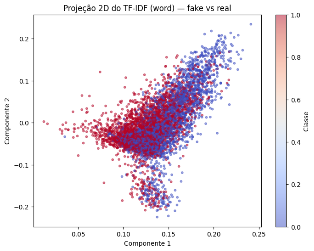
\includegraphics[keepaspectratio]{entregavel-final-img/fig10.png}}\pandocbounded{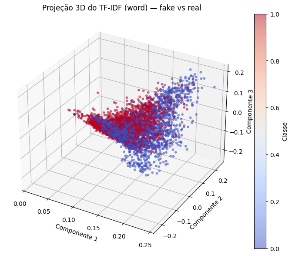
\includegraphics[keepaspectratio]{entregavel-final-img/fig11.png}}\pandocbounded{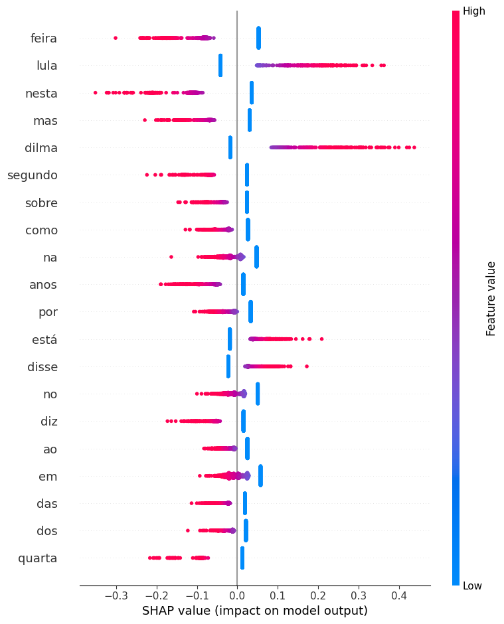
\includegraphics[keepaspectratio]{entregavel-final-img/fig12.png}}\pandocbounded{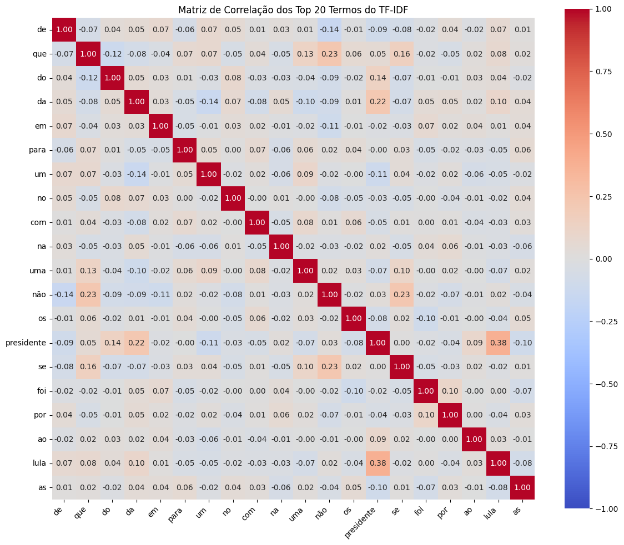
\includegraphics[keepaspectratio]{entregavel-final-img/fig13.png}}

\begin{center}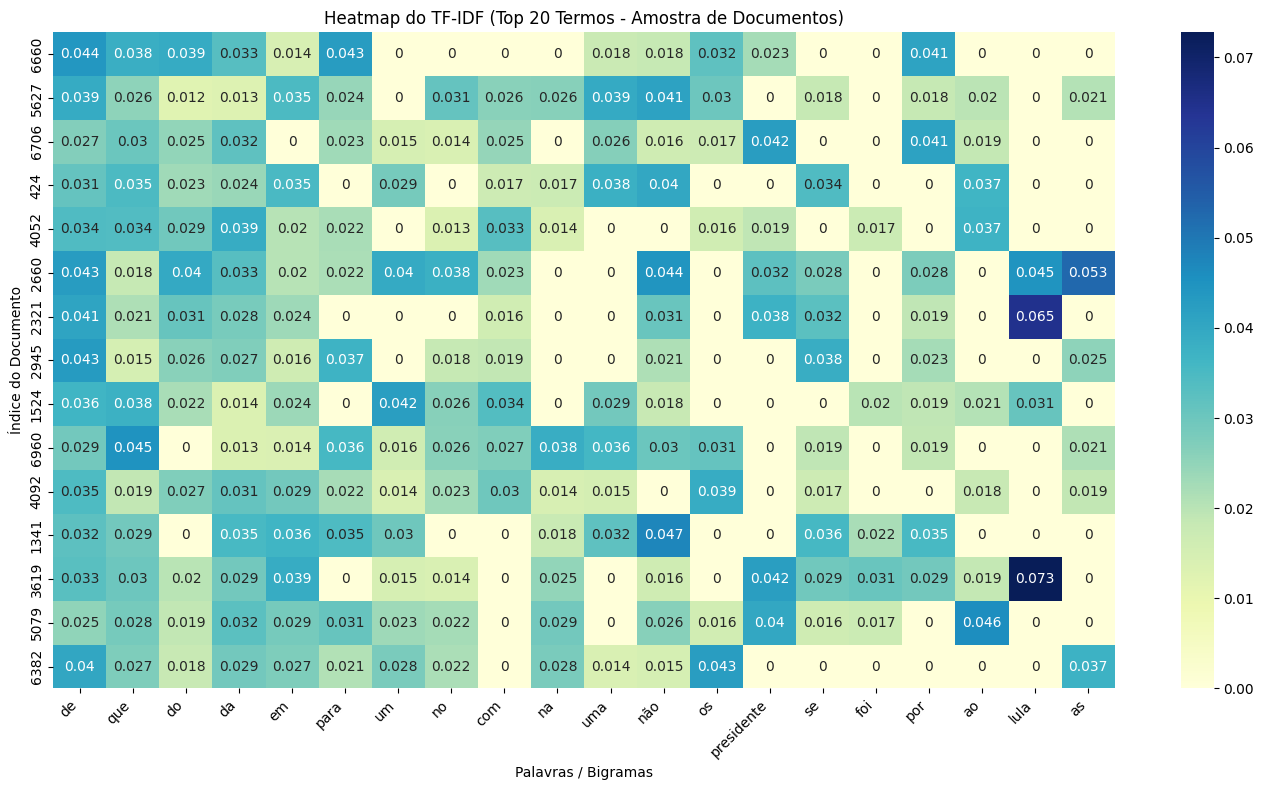
\includegraphics[width=0.95\linewidth,keepaspectratio]{entregavel-final-img/fig25.png}\\[2pt]{\small\emph{Heatmap do TF-IDF dos 20 termos mais frequentes em uma amostra de documentos. Fonte: notebook 02\_LR\_training.}}\end{center}

\begin{center}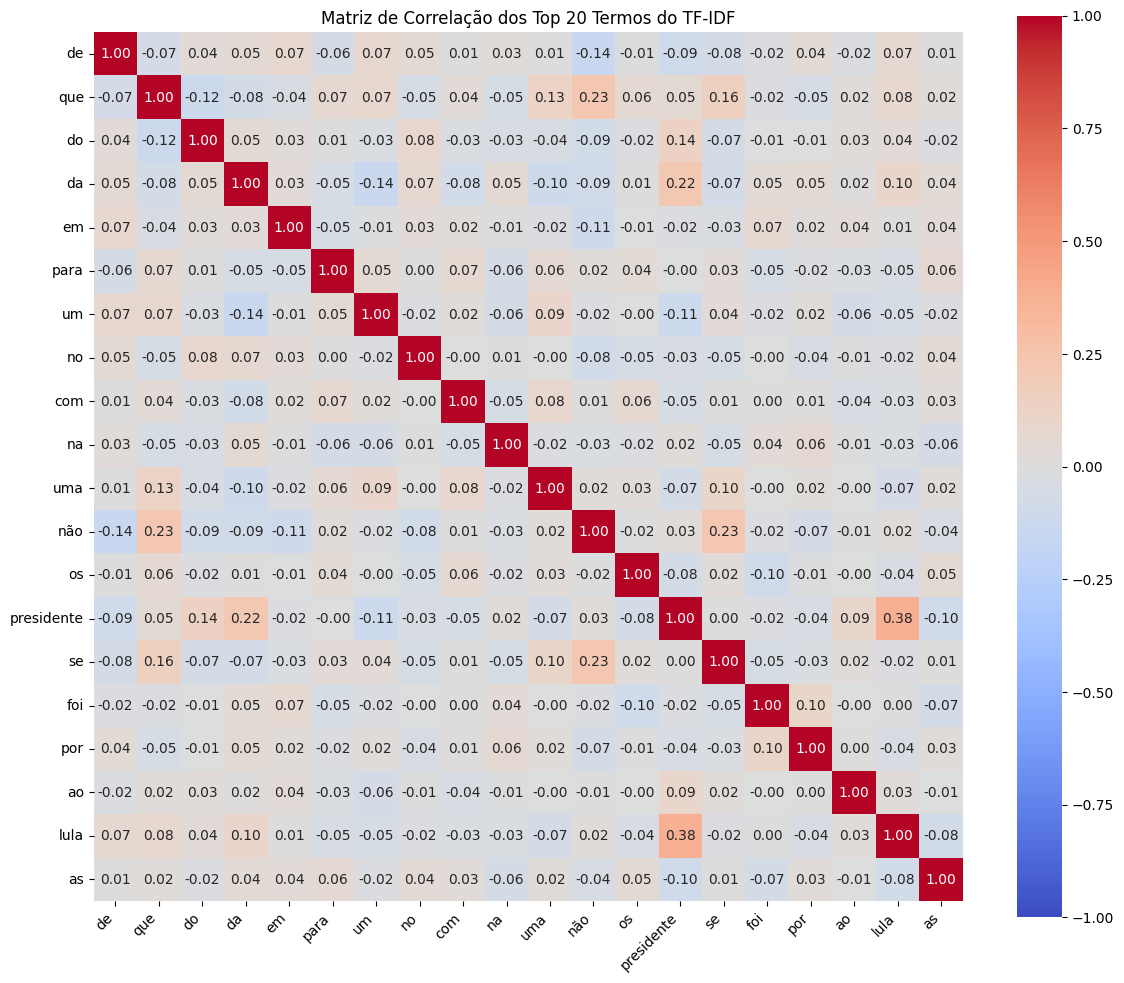
\includegraphics[width=0.7\linewidth,keepaspectratio]{entregavel-final-img/fig26.png}\\[2pt]{\small\emph{Matriz de correlação (Pearson) entre os 20 termos mais frequentes do TF-IDF. Fonte: notebook 02\_LR\_training.}}\end{center}

A configuração padrão (\texttt{txt\_word} + \texttt{txt\_char}) produz \textbf{114.301 atributos} para 5.760 documentos de treino, com cerca de 99,5\% de esparsidade. O vetorizador de palavras não remove acentos (o exemplo acima ilustra apenas a decomposição em n-gramas). A projeção 2D do TF-IDF com \texttt{TruncatedSVD} serve apenas para visualização: as duas primeiras componentes explicam \textasciitilde0,75\% da variância e misturam as classes (seção 5.8).

\subsection{5.4 Modelos treinados}\label{modelos-treinados}

\begin{quote}
\textbf{{[}NOTA{]}} As tabelas de validação cruzada e os resultados de teste desta seção vêm do \textbf{protocolo anterior} (truncamento em 200 palavras, sem normalização, 5 folds sem embaralhamento). Servem para comparar configurações entre si, mas \textbf{não são comparáveis} aos números das seções 5.5 a 5.9. Os notebooks \texttt{02}, \texttt{03} e \texttt{04} precisam ser reexecutados no pipeline atual para atualizar estas tabelas.
\end{quote}

\begin{quote}
\textbf{{[}PENDENTE{]}} Reexecutar \texttt{02\_LR\_training}, \texttt{03\_SVM\_training} e \texttt{04\_RF\_training} com o pipeline atual. No \texttt{04}, o título da seção diz "Regressão Logística" e a célula final chama \texttt{decision\_function}, que o RandomForest não possui; no \texttt{02}/\texttt{04} as células de CV estão comentadas, então os outputs não correspondem ao código.
\end{quote}

\subsubsection{SVM (Support Vector Machine)}\label{svm-support-vector-machine}

\paragraph{Racional de Escolha do Algoritmo}\label{racional-de-escolha-do-algoritmo}

A seleção do SVM, sob a variante de otimização linear (\textbf{LinearSVC}), fundamenta-se nas propriedades matemáticas inerentes ao domínio de Processamento de Linguagem Natural (PLN):

\begin{itemize}
\tightlist
\item
  \textbf{Alta Dimensionalidade e Esparsidade:} A representação vetorial do texto via TF-IDF gera matrizes com elevado volume de atributos (features), caracterizadas por alta densidade de zeros. O SVM é reconhecido pela robustez e eficiência computacional na navegação em espaços amostrais de alta dimensão.
\item
  \textbf{Maximização de Margem de Decisão:} O algoritmo delimita um hiperplano ótimo de separação, focado exclusivamente nos vetores de suporte, cujo as instâncias limítrofes entre as classes (Notícia Verdadeira vs. Notícia Falsa), mitigando o risco de \emph{overfitting} inerente a distribuições complexas.
\end{itemize}

\paragraph{Arquitetura de Implementação}\label{arquitetura-de-implementauxe7uxe3o}

A construção da solução adotou uma abordagem modular, encapsulada e escalável via scikit-learn.

\subparagraph{Configuração e Hiperparâmetros do Estimador}\label{configurauxe7uxe3o-e-hiperparuxe2metros-do-estimador}

O núcleo de classificação foi parametrizado com as seguintes diretrizes:

\begin{itemize}
\tightlist
\item
  \textbf{class\_weight=\textquotesingle balanced\textquotesingle{}}: Ajusta a função de perda inversamente proporcional às frequências das classes. Como o conjunto é balanceado (3.600/3.600), o parâmetro não tem efeito prático; o grid search confirmou resultados idênticos com e sem ele.
\item
  \textbf{max\_iter=2000:} Expansão do teto de iterações para assegurar a convergência do solucionador numérico sobre matrizes de alta complexidade.
\item
  \textbf{random\_state=42:} Fixação de semente estocástica para garantir a reprodutibilidade integral dos experimentos.
\end{itemize}

\subparagraph{Pipeline de Extração de Atributos}\label{pipeline-de-extrauxe7uxe3o-de-atributos}

Para mitigar vazamentos de dados (\emph{data leakage}), o estimador foi integrado a um pipeline alimentado por um \textbf{ColumnTransformer}, avaliado em quatro configurações incrementais de extração:

\begin{itemize}
\tightlist
\item
  \textbf{word}: Vetorização n-grama baseada estritamente em palavras.
\item
  \textbf{word+char}: Combinação de n-gramas de palavras e n-gramas de caracteres.
\item
  \textbf{word+meta}: Vetorização de palavras acoplada a metadados linguísticos e estilísticos (devidamente normalizados).
\item
  \textbf{word+char+meta}: Integração unificada de todas as representações vetoriais.
\end{itemize}

\subparagraph{Calibração de probabilidades}\label{calibrauxe7uxe3o-de-probabilidades}

O \textbf{LinearSVC} retorna apenas a distância ao hiperplano. Para entregar uma pontuação de 0 a 1 ao sistema, o pipeline de produção (\texttt{modelo\_olimpo.py}, seção 5.11) envolve o estimador em \texttt{CalibratedClassifierCV} com método \textbf{sigmoide (Platt)}, \texttt{StratifiedKFold(5)} e \texttt{ensemble=False}. Os notebooks 02 a 12 usam o \texttt{decision\_function} (ROC-AUC) e não a calibração.

\paragraph{Vantagens}\label{vantagens}

Se comporta bem em dados de alta dimensionalidade, muito utilizado para classificação de texto e imagem, com boa regularização por margem e consegue construir fronteiras lineares e não lineares.

\paragraph{Desvantagens}\label{desvantagens}

Depende de um poder computacional mais robusto que os outros modelos mais simples, o ajuste de kernel só é necessário nas variantes não lineares (\texttt{SVC}); o \texttt{LinearSVC} adotado não usa kernel. Os kernels RBF e polinomial foram testados no notebook 09 (seção 5.8).

\paragraph{Avaliação Empírica de Desempenho}\label{avaliauxe7uxe3o-empuxedrica-de-desempenho}

A validação foi conduzida utilizando Validação Cruzada Estratificada (k=5), avaliando o poder de generalização do modelo diante de dados não observados.

{\def\LTcaptype{none} % do not increment counter
\begin{longtable}[]{@{}
  >{\raggedright\arraybackslash}p{(\linewidth - 8\tabcolsep) * \real{0.2804}}
  >{\raggedright\arraybackslash}p{(\linewidth - 8\tabcolsep) * \real{0.1776}}
  >{\raggedright\arraybackslash}p{(\linewidth - 8\tabcolsep) * \real{0.1776}}
  >{\raggedright\arraybackslash}p{(\linewidth - 8\tabcolsep) * \real{0.1869}}
  >{\raggedright\arraybackslash}p{(\linewidth - 8\tabcolsep) * \real{0.1776}}@{}}
\toprule\noalign{}
\endhead
\bottomrule\noalign{}
\endlastfoot
\textbf{Configuração de Features} & \textbf{F1-Macro} & \textbf{Acurácia} & \textbf{Precisão Macro} & \textbf{Recall Macro} \\
\textbf{\texttt{word\ +\ char\ +\ meta}} & 0.9554 (± 0.0155) & 0.9554 (± 0.0154) & 0.9568 (± 0.0135) & 0.9554 (± 0.0154) \\
\textbf{\texttt{word\ +\ char}} & 0.9516 (± 0.0184) & 0.9517 (± 0.0183) & 0.9538 (± 0.0158) & 0.9517 (± 0.0183) \\
\textbf{\texttt{word\ +\ meta}} & 0.9384 (± 0.0153) & 0.9385 (± 0.0152) & 0.9404 (± 0.0133) & 0.9385 (± 0.0152) \\
\textbf{\texttt{word}} & 0.9352 (± 0.0142) & 0.9353 (± 0.0140) & 0.9380 (± 0.0114) & 0.9353 (± 0.0140) \\
\end{longtable}
}

\paragraph{Avaliação dos resultados com os dados de testes}\label{avaliauxe7uxe3o-dos-resultados-com-os-dados-de-testes}

O desempenho no teste ficou dentro de um desvio-padrão da validação cruzada, o que indica que a escolha da configuração não gerou \emph{seleção} excessiva sobre o treino. Isso não implica generalização para outros corpora (seção 5.9). No protocolo anterior, o LinearSVC teve o melhor desempenho entre os três modelos.

\begin{quote}
\textbf{{[}PENDENTE{]}} A contagem original ("64 erros em 1.440: 49 falsas→verdadeiras e 15 verdadeiras→falsas") não foi localizada em nenhum notebook do repositório; o único teste de SVM com output salvo (word+char+meta) tem F1-macro de 0,9465 (acurácia 0,9465, ROC-AUC 0,9906). Reexecutar e registrar a matriz de confusão.
\end{quote}

\subsubsection{Por que funciona no nosso caso?}\label{por-que-funciona-no-nosso-caso}

O SVM com kernel linear obteve o melhor desempenho no nosso modelo de detecção de Fake News porque é algoritmicamente desenhado para lidar com a extrema alta dimensionalidade e esparsidade dos dados gerados pelo TF-IDF. Ao combinarmos \emph{n-grams} de palavras, caracteres e metadados, criamos um espaço com milhares de variáveis onde as classes (Verdadeiro e Falso) tornam-se naturalmente linearmente separáveis. Enquanto modelos baseados em árvores sofrem de \emph{overfitting} ao tentar memorizar ruídos e regras muito específicas nesse cenário, o SVM foca estritamente em traçar um hiperplano que maximize a margem de separação entre as classes, ignorando os exemplos óbvios e ajustando-se apenas aos textos mais difíceis de classificar (vetores de suporte). Isso torna o modelo altamente robusto, permitindo que ele some centenas de sutis evidências linguísticas de forma estável para determinar a veracidade de uma notícia dentro do corpus.

\subsubsection{Notebook com o código do treinamento e cross validation da SVM}\label{notebook-com-o-cuxf3digo-do-treinamento-e-cross-validation-da-svm}

\url{https://colab.research.google.com/drive/1g3B2vDnUg7f7ENvulFNFPOygQ1jzoG5F?usp=sharing}

\subsubsection{Random Forest}\label{random-forest}

\paragraph{Racional de Utilização do Algoritmo}\label{racional-de-utilizauxe7uxe3o-do-algoritmo}

A inclusão do \emph{Random Forest} (RandomForestClassifier) no escopo experimental do projeto fundamenta-se na avaliação de estimadores baseados em \emph{Ensemble Learning} (Aprendizado em Conjunto) e no particionamento não-linear do espaço de atributos:

\begin{itemize}
\tightlist
\item
  \textbf{Arquitetura de Ensemble por Bagging (\emph{Bootstrap Aggregating}):} O algoritmo combina múltiplos estimadores fracos (árvores de decisão individuais) treinados sobre subamostras do conjunto de dados. Essa votação reduz drasticamente a variância do modelo, mitigando o risco de \emph{overfitting} comum em árvores de decisão isoladas diante de ruídos textuais.
\item
  \textbf{Mapeamento de Regras Não-Lineares e Interações Complexas:} Diferente de modelos lineares, o \emph{Random Forest} divide o espaço de busca por meio de cortes ortogonais nos nós das árvores. Essa propriedade permite identificar dependências condicionais complexas entre variáveis (ex.: a combinação simultânea de alta taxa\_maiusculas com baixa diversidade) sem a necessidade de engenharia manual de termos de interação.
\item
  \textbf{Invariância à Escala de Atributos:} O processo de divisão dos nós depende estritamente da ordem relativa dos valores e não de sua magnitude absoluta. Essa característica confere robustez ao modelo ao processar vetores heterogêneos que agrupam TF-IDF (valores entre 0 e 1) e metadados numéricos não-normalizados.
\end{itemize}

\paragraph{Arquitetura de Implementação}\label{arquitetura-de-implementauxe7uxe3o-1}

A construção do modelo seguiu o mesmo padrão modular e auditável, garantindo isonomia na comparação de desempenho através do scikit-learn.

\subparagraph{Configuração e Hiperparâmetros do Estimador}\label{configurauxe7uxe3o-e-hiperparuxe2metros-do-estimador-1}

O modelo núcleo foi instanciado com a seguinte parametrização:

\begin{itemize}
\tightlist
\item
  n\_estimators=100: Definição de um \emph{ensemble} composto por 100 árvores de decisão independentes, assegurando estabilidade estatística e convergência na distribuição das votações.
\item
  random\_state=42: Fixação da semente estocástica para garantir a reprodutibilidade integral dos sementes e ramificações geradas.
\item
  max\_features=\textquotesingle sqrt\textquotesingle: Restrição do número de atributos avaliados em cada nó à raiz quadrada do total de \emph{features}, promovendo a descorrelação entre as árvores da floresta.
\end{itemize}

\subparagraph{Pipeline de Extração de Atributos}\label{pipeline-de-extrauxe7uxe3o-de-atributos-1}

Para prevenir o vazamento de dados, o \emph{Random Forest} atuou como o estimador final de um Pipeline acoplado ao ColumnTransformer, avaliado sob quatro arranjos incrementais de vetorização:

\begin{itemize}
\tightlist
\item
  \textbf{word}
\item
  \textbf{word+char}
\item
  \textbf{word+meta}
\item
  \textbf{word+char+meta}
\end{itemize}

\subparagraph{Suporte nativo à explicabilidade (SHAP / TreeExplainer)}\label{suporte-nativo-uxe0-explicabilidade-shap-treeexplainer}

A estrutura baseada em árvores do \emph{Random Forest} permite a integração com \texttt{shap.TreeExplainer} e o cálculo exato dos valores SHAP de interação.

\begin{quote}
\textbf{{[}PENDENTE{]}} Os notebooks do repositório não contêm esse cálculo para o Random Forest (o \texttt{TreeExplainer} aparece apenas em um notebook histórico não supervisionado, e o SHAP supervisionado usa \texttt{LinearExplainer} sobre a Regressão Logística). Os gráficos da seção 5.7 vêm de um notebook externo que precisa ser versionado.
\end{quote}

\paragraph{Vantagens}\label{vantagens-1}

Possui um bom desempenho com variedade dos dados, bom comportamento com dados não lineares, baixo risco de overfitting.

\paragraph{Desvantagens}\label{desvantagens-1}

Entre os modelos selecionados não é o que menos precisa de recurso computacional, a importância das variáveis não significa causalidade obrigatoriamente.

\paragraph{Avaliação Empírica de Desempenho}\label{avaliauxe7uxe3o-empuxedrica-de-desempenho-1}

A validação do modelo foi conduzida via Validação Cruzada Estratificada (k=5), medindo o poder de generalização diante de dados não observados.

{\def\LTcaptype{none} % do not increment counter
\begin{longtable}[]{@{}
  >{\raggedright\arraybackslash}p{(\linewidth - 8\tabcolsep) * \real{0.2804}}
  >{\raggedright\arraybackslash}p{(\linewidth - 8\tabcolsep) * \real{0.1776}}
  >{\raggedright\arraybackslash}p{(\linewidth - 8\tabcolsep) * \real{0.1776}}
  >{\raggedright\arraybackslash}p{(\linewidth - 8\tabcolsep) * \real{0.1869}}
  >{\raggedright\arraybackslash}p{(\linewidth - 8\tabcolsep) * \real{0.1776}}@{}}
\toprule\noalign{}
\endhead
\bottomrule\noalign{}
\endlastfoot
\textbf{Configuração de Features} & \textbf{F1-Macro} & \textbf{Acurácia} & \textbf{Precisão Macro} & \textbf{Recall Macro} \\
\textbf{\texttt{word\ +\ char\ +\ meta}} & 0.9320 (± 0.0140) & 0.9321 (± 0.0138) & 0.9345 (± 0.0122) & 0.9320 (± 0.0138) \\
\textbf{\texttt{word\ +\ char}} & 0.9285 (± 0.0162) & 0.9286 (± 0.0160) & 0.9302 (± 0.0145) & 0.9286 (± 0.0160) \\
\textbf{\texttt{word\ +\ meta}} & 0.9150 (± 0.0155) & 0.9151 (± 0.0153) & 0.9180 (± 0.0130) & 0.9151 (± 0.0153) \\
\textbf{\texttt{word}} & 0.9112 (± 0.0135) & 0.9113 (± 0.0132) & 0.9142 (± 0.0110) & 0.9113 (± 0.0132) \\
\end{longtable}
}

\paragraph{Avaliação dos resultados com os dados de testes}\label{avaliauxe7uxe3o-dos-resultados-com-os-dados-de-testes-1}

O resultado no teste foi cerca de 0,7 ponto percentual abaixo da validação cruzada, dentro de um desvio-padrão, o que é consistente. O modelo errou 113 textos: 83 falsas classificadas como verdadeiras e 30 verdadeiras classificadas como falsas. Foi o modelo com mais erros dos três, e o que mais deixou notícias falsas passarem (recall da classe falsa de 0,8847).

\begin{center}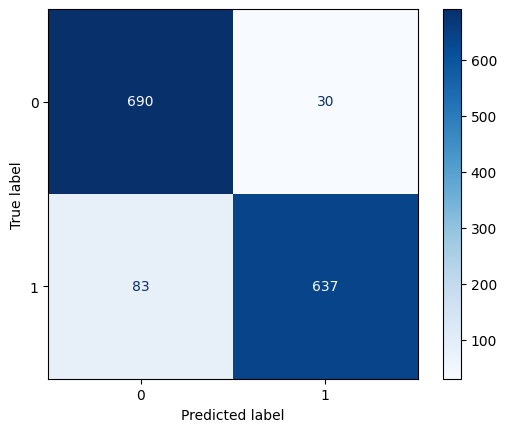
\includegraphics[width=0.5\linewidth,keepaspectratio]{entregavel-final-img/fig23.png}\\[2pt]{\small\emph{Matriz de confusão do Random Forest no teste (1.440 textos; protocolo anterior). Fonte: notebook 04\_RF\_training.}}\end{center}

\paragraph{Notebook com o código do treinamento e cross validation da random forest}\label{notebook-com-o-cuxf3digo-do-treinamento-e-cross-validation-da-random-forest}

\url{https://colab.research.google.com/drive/12TiiqYNQwJJ5eN6Se8psifMTo8N0NADp?usp=sharing}

\subsubsection{Regressão Logística}\label{regressuxe3o-loguxedstica}

\paragraph{Racional de Utilização do Algoritmo}\label{racional-de-utilizauxe7uxe3o-do-algoritmo-1}

A adoção da \emph{Regressão Logística} (LogisticRegression) no pipeline experimental teve como propósito estabelecer a \textbf{linha de base (\emph{baseline})} do projeto. Em Processamento de Linguagem Natural (PLN), estimadores lineares probabilísticos fornecem o patamar mínimo de desempenho a ser superado por arquiteturas mais complexas:

\begin{itemize}
\tightlist
\item
  \textbf{Interpretabilidade Direta e Probabilidades Nativas:} O modelo aplica a função sigmoide \textbf{σ(z) = 1 / (1 + e⁻ᶻ)} sobre a combinação linear dos atributos, mapeando a saída diretamente para o intervalo entre 0 e 1 (0\% a 100\%). Ao contrário do LinearSVC, a Regressão Logística entrega pontuações de probabilidade nativas sem a necessidade de métodos de calibração secundários. Além disso, a inspeção direta dos coeficientes (pesos \emph{beta}) permite auditar com clareza a influência de cada n-grama ou métrica na classificação do texto como desinformação.
\item
  \textbf{Eficiência Computacional e Navegação em Espaços Esparsos:} A otimização convexa por algoritmos de gradiente opera com extrema rapidez em matrizes esparsas de alta dimensão geradas pelo TF-IDF, oferecendo um excelente balanço entre custo computacional e acurácia preditiva.
\end{itemize}

\paragraph{Arquitetura de Implementação}\label{arquitetura-de-implementauxe7uxe3o-2}

A validação da Regressão Logística seguiu rigorosamente a mesma esteira de pré-processamento e partição utilizada nos demais estimadores, assegurando isonomia nos testes do scikit-learn.

\subparagraph{Configuração e Hiperparâmetros do Estimador}\label{configurauxe7uxe3o-e-hiperparuxe2metros-do-estimador-2}

O modelo núcleo foi parametrizado com as seguintes diretrizes:

\begin{itemize}
\tightlist
\item
  class\_weight=\textquotesingle balanced\textquotesingle: penaliza os erros de forma inversamente proporcional à frequência das classes; sem efeito prático aqui, pois o conjunto é balanceado.
\item
  max\_iter=1000: Expansão do teto de iterações do solver de otimização para garantir a convergência dos coeficientes numéricos no espaço multidimensional de features.
\item
  O \texttt{random\_state} não é fixado no solver \texttt{lbfgs} (determinístico), diferentemente do LinearSVC e do Random Forest.
\end{itemize}

\subparagraph{Pipeline de Extração de Atributos}\label{pipeline-de-extrauxe7uxe3o-de-atributos-2}

Para mitigar o risco de vazamento de dados, o estimador atuou como o nó final de um Pipeline acoplado ao ColumnTransformer, avaliado sob quatro arranjos incrementais:

\begin{itemize}
\tightlist
\item
  \textbf{word}
\item
  \textbf{word+char}
\item
  \textbf{word+meta}
\item
  \textbf{word+char+meta}
\end{itemize}

\paragraph{Vantagens}\label{vantagens-2}

Precisa de pouco desempenho computacional, muito bom com dados lineares, fácil compreensão.

\paragraph{Desvantagens}\label{desvantagens-2}

Limitado para fronteiras não lineares. Quanto ao ajuste, o gap treino--validação com C=1 é de 0,067 (LinearSVC: 0,070), ou seja, tão sujeito a superajuste no espaço TF-IDF quanto o SVM.

\paragraph{Avaliação Empírica de Desempenho}\label{avaliauxe7uxe3o-empuxedrica-de-desempenho-2}

{\def\LTcaptype{none} % do not increment counter
\begin{longtable}[]{@{}
  >{\raggedright\arraybackslash}p{(\linewidth - 8\tabcolsep) * \real{0.1875}}
  >{\raggedright\arraybackslash}p{(\linewidth - 8\tabcolsep) * \real{0.1875}}
  >{\raggedright\arraybackslash}p{(\linewidth - 8\tabcolsep) * \real{0.1875}}
  >{\raggedright\arraybackslash}p{(\linewidth - 8\tabcolsep) * \real{0.2375}}
  >{\raggedright\arraybackslash}p{(\linewidth - 8\tabcolsep) * \real{0.2000}}@{}}
\toprule\noalign{}
\begin{minipage}[b]{\linewidth}\raggedright
\textbf{Feature Set}
\end{minipage} & \begin{minipage}[b]{\linewidth}\raggedright
\textbf{f1\_macro}
\end{minipage} & \begin{minipage}[b]{\linewidth}\raggedright
\textbf{accuracy}
\end{minipage} & \begin{minipage}[b]{\linewidth}\raggedright
\textbf{precision\_macro}
\end{minipage} & \begin{minipage}[b]{\linewidth}\raggedright
\textbf{recall\_macro}
\end{minipage} \\
\midrule\noalign{}
\endhead
\bottomrule\noalign{}
\endlastfoot
word & 0.9243 ± 0.0048 & 0.9243 ± 0.0048 & 0.9250 ± 0.0044 & 0.9243 ± 0.0048 \\
word+char & 0.9474 ± 0.0031 & 0.9474 ± 0.0031 & 0.9483 ± 0.0029 & 0.9474 ± 0.0031 \\
word+meta & 0.9006 ± 0.0082 & 0.9007 ± 0.0081 & 0.9020 ± 0.0079 & 0.9007 ± 0.0081 \\
word+char+meta & 0.9326 ± 0.0016 & 0.9326 ± 0.0016 & 0.9336 ± 0.0016 & 0.9326 ± 0.0016 \\
\end{longtable}
}

\paragraph{Avaliação dos resultados com os dados de teste}\label{avaliauxe7uxe3o-dos-resultados-com-os-dados-de-teste}

O F1-Macro no teste ficou 0,3 ponto percentual abaixo da validação cruzada, dentro de um desvio-padrão. O modelo errou 80 textos: 59 falsas classificadas como verdadeiras e 21 verdadeiras classificadas como falsas.

\begin{center}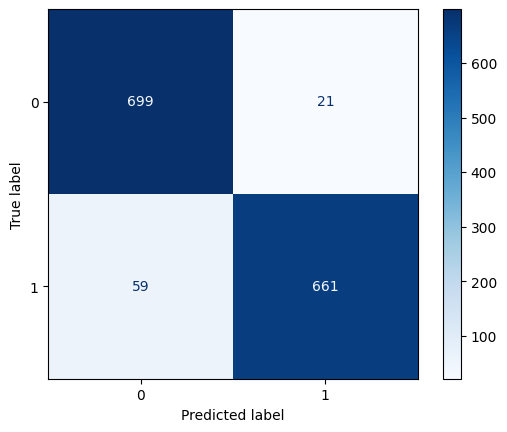
\includegraphics[width=0.5\linewidth,keepaspectratio]{entregavel-final-img/fig22.png}\\[2pt]{\small\emph{Matriz de confusão da Regressão Logística no teste (1.440 textos; protocolo anterior). Fonte: notebook 02\_LR\_training.}}\end{center}

\paragraph{Notebook com o código do treinamento e cross validation da Regressão Logística}\label{notebook-com-o-cuxf3digo-do-treinamento-e-cross-validation-da-regressuxe3o-loguxedstica}

\url{https://colab.research.google.com/drive/1sAjVrmOaKkYbtNSGiiHIP6WV745ySN1P?usp=sharing}

\subsubsection{Modelo baseline}\label{modelo-baseline-1}

Adotamos como baseline a Regressão Logística com TF-IDF de palavras (unigramas e bigramas) aplicado ao texto truncado, com class\_weight=\textquotesingle balanced\textquotesingle, max\_iter=1000 e random\_state=42. Esse modelo estabelece o patamar mínimo de desempenho a ser superado: F1-Macro de 0.9243 em validação cruzada (k=5, protocolo anterior; \textbf{{[}PENDENTE{]}} recalcular no pipeline atual).

Um modelo mais complexo só se justifica se superar esse patamar de forma consistente, considerando o custo computacional e a perda de interpretabilidade.

\paragraph{Escolha do modelo como baseline}\label{escolha-do-modelo-como-baseline}

\textbf{Simplicidade e Interpretabilidade:} os coeficientes podem ser analisados diretamente, o que permite explicar quais n-gramas contribuem para a classificação de uma notícia como desinformação.

\textbf{Probabilidades Nativas:} a saída é uma probabilidade entre 0 e 1 sem etapa de calibração, ao contrário do LinearSVC.

\textbf{Eficiência em Espaços Esparsos:} treina rapidamente sobre as matrizes de alta dimensão geradas pelo TF-IDF.

\textbf{Dois Níveis de Referência}

Piso (word): 0.9243, a Regressão Logística com o menor conjunto de features.

Melhor configuração do baseline (word+char): 0.9474, o teto que a Regressão Logística atinge nos experimentos.

Os n-gramas de caractere elevaram o F1 em +0.0231 sobre o piso. Já os metadados estilométricos reduziram o desempenho na Regressão Logística: −0.0237 sobre word e −0.0148 sobre word+char.

\subsection{5.5 Resultados no protocolo atual: regularização (C) e poda de vocabulário}\label{resultados-no-protocolo-atual-regularizauxe7uxe3o-c-e-poda-de-vocabuluxe1rio}

Todos os experimentos desta seção e das seguintes usam os mesmos dados (\texttt{X\_tr}), os mesmos folds (\texttt{StratifiedKFold(5,\ shuffle=True,\ random\_state=42)}) e a configuração word+char. O teste (\texttt{X\_te}) não é usado. O \textbf{gap} é F1 de treino − F1 de validação.

\subsubsection{\texorpdfstring{Regularização (\texttt{06\_regularizacao\_C})}{Regularização (06\_regularizacao\_C)}}\label{regularizauxe7uxe3o-06_regularizacao_c}

{\def\LTcaptype{none} % do not increment counter
\begin{longtable}[]{@{}llllll@{}}
\toprule\noalign{}
modelo & C & f1\_treino & f1\_cv & f1\_cv\_std & gap \\
\midrule\noalign{}
\endhead
\bottomrule\noalign{}
\endlastfoot
LinearSVC & 0.01 & 0.9211 & 0.8802 & 0.0123 & 0.0409 \\
LinearSVC & 0.03 & 0.9564 & 0.9024 & 0.0150 & 0.0540 \\
LinearSVC & 0.1 & 0.9866 & 0.9203 & 0.0142 & 0.0663 \\
LinearSVC & 0.3 & 0.9997 & 0.9264 & 0.0111 & 0.0733 \\
LinearSVC & 1 & 1.0000 & 0.9295 & 0.0099 & 0.0705 \\
LinearSVC & 3 & 1.0000 & 0.9283 & 0.0074 & 0.0717 \\
LinearSVC & 10 & 1.0000 & 0.9283 & 0.0066 & 0.0717 \\
Regressão Logística & 0.01 & 0.8703 & 0.8417 & 0.0101 & 0.0285 \\
Regressão Logística & 0.03 & 0.8942 & 0.8577 & 0.0122 & 0.0365 \\
Regressão Logística & 0.1 & 0.9261 & 0.8837 & 0.0129 & 0.0425 \\
Regressão Logística & 0.3 & 0.9576 & 0.9019 & 0.0146 & 0.0556 \\
Regressão Logística & 1 & 0.9851 & 0.9182 & 0.0136 & 0.0669 \\
Regressão Logística & 3 & 0.9987 & 0.9241 & 0.0125 & 0.0746 \\
Regressão Logística & 10 & 1.0000 & 0.9281 & 0.0109 & 0.0719 \\
\end{longtable}
}

\begin{itemize}
\tightlist
\item
  \textbf{LinearSVC}: com C ≤ 0,03 o modelo entra em \emph{underfitting} (F1 0,8802 em C=0,01). O máximo está em \textbf{C=1 (0,9295 ± 0,0099)}; C=3 e C=10 saturam o treino em 1,0 sem ganho na validação. O C padrão é o ponto ótimo.
\item
  \textbf{Regressão Logística}: o F1 cresce de forma monotônica até \textbf{C=10 (0,9281 ± 0,0109)}, praticamente empatando com o LinearSVC. Em espaços esparsos de alta dimensão a LR se beneficia de regularização mais fraca que o padrão.
\item
  O gap mínimo útil gira em torno de 0,07 e não se fecha com regularização sem perda de F1.
\end{itemize}

\subsubsection{\texorpdfstring{Poda de vocabulário (\texttt{05\_feature\_dim\_analysis}, \texttt{min\_df})}{Poda de vocabulário (05\_feature\_dim\_analysis, min\_df)}}\label{poda-de-vocabuluxe1rio-05_feature_dim_analysis-min_df}

F1 de validação cruzada do \textbf{LinearSVC} para cada par (\texttt{min\_df} de palavras × \texttt{min\_df} de caracteres); a configuração atual é word=2, char=3.

{\def\LTcaptype{none} % do not increment counter
\begin{longtable}[]{@{}lllll@{}}
\toprule\noalign{}
word ~char & char=1 & char=3 & char=5 & char=10 \\
\midrule\noalign{}
\endhead
\bottomrule\noalign{}
\endlastfoot
1 & 0.9290 & 0.9279 & 0.9279 & 0.9286 \\
2 & 0.9292 & 0.9295 & 0.9293 & 0.9293 \\
5 & 0.9279 & 0.9276 & 0.9276 & 0.9272 \\
10 & 0.9259 & 0.9260 & 0.9262 & 0.9259 \\
\end{longtable}
}

Número médio de atributos por combinação:

{\def\LTcaptype{none} % do not increment counter
\begin{longtable}[]{@{}lllll@{}}
\toprule\noalign{}
word ~char & char=1 & char=3 & char=5 & char=10 \\
\midrule\noalign{}
\endhead
\bottomrule\noalign{}
\endlastfoot
1 & 344.416 & 279.670 & 265.043 & 251.039 \\
2 & 179.046 & 114.301 & 99.673 & 85.670 \\
5 & 142.415 & 77.669 & 63.042 & 49.039 \\
10 & 133.414 & 68.668 & 54.041 & 40.037 \\
\end{longtable}
}

Com o LinearSVC, reduzir de 114 mil para \textasciitilde40 mil atributos (\texttt{min\_df} 10/10) custa apenas \textasciitilde0,003 de F1 (0,9259 contra 0,9295), dentro do desvio entre folds (\textasciitilde0,010). Na Regressão Logística a poda melhora levemente o F1 (0,9182 → 0,9205 em 5/5) e reduz o gap, também dentro do ruído.

\begin{center}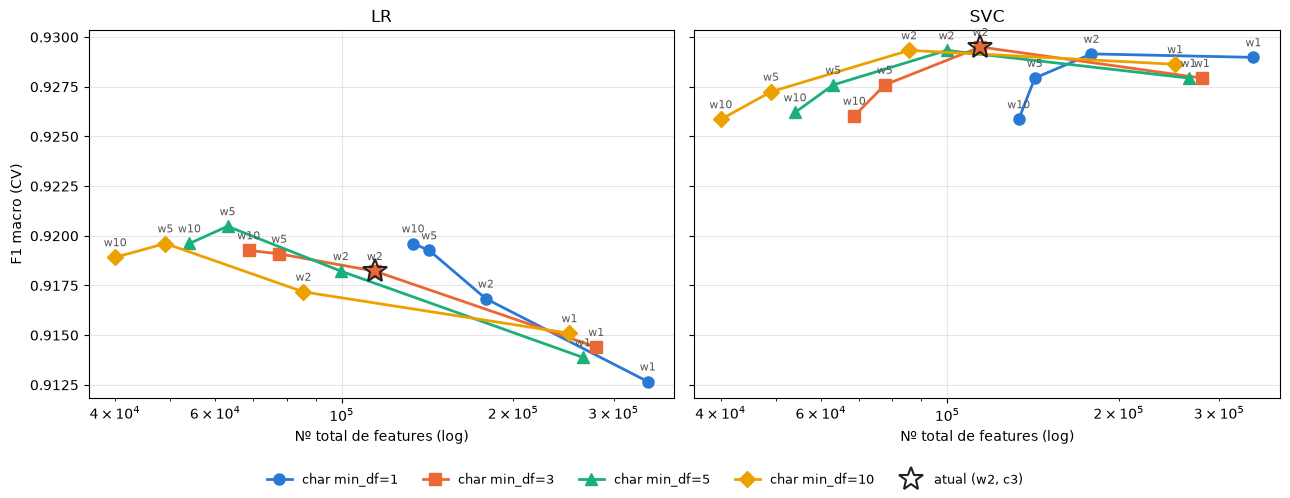
\includegraphics[width=0.95\linewidth,keepaspectratio]{entregavel-final-img/fig30.png}\\[2pt]{\small\emph{F1 macro (CV) em função do número total de atributos, por combinação de min\_df. A estrela marca a configuração atual. Fonte: notebook 05\_feature\_dim\_analysis.}}\end{center}

\begin{center}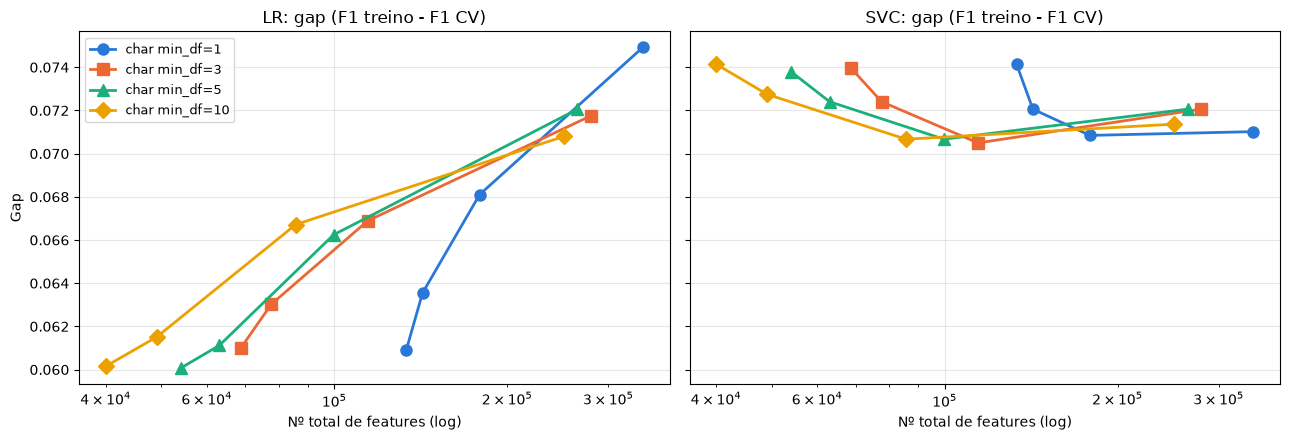
\includegraphics[width=0.95\linewidth,keepaspectratio]{entregavel-final-img/fig31.png}\\[2pt]{\small\emph{Gap (F1 treino − F1 CV) em função do número total de atributos. Fonte: notebook 05\_feature\_dim\_analysis.}}\end{center}

\subsection{5.6 Metadados: do corpus e morfossintáticos (spaCy)}\label{metadados-do-corpus-e-morfossintuxe1ticos-spacy}

\subsubsection{Metadados do corpus}\label{metadados-do-corpus}

Os atributos do corpus (\texttt{num\_verbos}, \texttt{pausalidade}, \texttt{diversidade} etc.) são calculados pelo NILC sobre o \textbf{texto completo}, enquanto o TF-IDF vê apenas as 100 primeiras palavras; as taxas são normalizadas pelo \texttt{num\_palavras} do texto completo. Esses atributos \textbf{não existem} para notícias novas inseridas pelo usuário nem para o FakeRecogna.

Resultados registrados:

\begin{itemize}
\tightlist
\item
  Na \textbf{Regressão Logística} (curva de aprendizado, protocolo anterior): word+meta fica 2,4 pontos abaixo de word e word+char+meta fica 1,5 ponto abaixo de word+char. No LinearSVC e no Random Forest a diferença é de no máximo \textasciitilde0,4 ponto, dentro do desvio. A hipótese em investigação é a diferença de escala entre o bloco denso padronizado e o TF-IDF sob regularização L2.
\item
  No \textbf{grid search} da branch \texttt{feat/taxa\_stop\_words} (ainda não integrada; 3 folds, C ∈ \{0,1; 1; 10\}, bloco de metadados acrescido de \texttt{taxa\_stop\_words}), o LinearSVC com word+char+meta e C=10 obteve \textbf{F1 0,9415 ± 0,0026}, contra 0,9276 ± 0,0024 do word+char (C=1) e 0,9094 do word. Esses valores estão em protocolo de 3 folds e não são comparáveis aos de 5 folds.
\end{itemize}

\begin{quote}
\textbf{{[}NOTA{]}} As duas evidências não são comparáveis entre si: uma é a LR no protocolo anterior e a outra é o SVM em 3 folds com um bloco de metadados diferente. O bloco avaliado no protocolo atual, em 5 folds e com teste externo, é o de metadados spaCy (abaixo).
\end{quote}

\subsubsection{\texorpdfstring{Extração morfossintática com spaCy (branch \texttt{fix-metadados})}{Extração morfossintática com spaCy (branch fix-metadados)}}\label{extrauxe7uxe3o-morfossintuxe1tica-com-spacy-branch-fix-metadados}

A branch \texttt{fix-metadados} (Ana Laura Alves Cordeiro) conta, com o \texttt{pt\_core\_news\_sm}, as classes gramaticais (POS) e as relações de dependência sintática (DEP) de cada classe do Fake.br, sobre o texto completo, e grava a proporção sobre o total de tokens (799.162 tokens falsos e 4.582.307 verdadeiros). Principais diferenças:

{\def\LTcaptype{none} % do not increment counter
\begin{longtable}[]{@{}
  >{\raggedright\arraybackslash}p{(\linewidth - 6\tabcolsep) * \real{0.2500}}
  >{\raggedright\arraybackslash}p{(\linewidth - 6\tabcolsep) * \real{0.2500}}
  >{\raggedright\arraybackslash}p{(\linewidth - 6\tabcolsep) * \real{0.2500}}
  >{\raggedright\arraybackslash}p{(\linewidth - 6\tabcolsep) * \real{0.2500}}@{}}
\toprule\noalign{}
\begin{minipage}[b]{\linewidth}\raggedright
Atributo
\end{minipage} & \begin{minipage}[b]{\linewidth}\raggedright
Falsas
\end{minipage} & \begin{minipage}[b]{\linewidth}\raggedright
Verdadeiras
\end{minipage} & \begin{minipage}[b]{\linewidth}\raggedright
Leitura
\end{minipage} \\
\midrule\noalign{}
\endhead
\bottomrule\noalign{}
\endlastfoot
POS \texttt{SPACE} & 2,88\% & 0,29\% & artefato de formatação da fonte \\
DEP \texttt{dep} & 3,21\% & 0,64\% & mesmo artefato (tokens de espaço sem relação sintática) \\
DEP \texttt{ROOT} & 5,94\% & 4,93\% & frases mais curtas nas falsas \\
POS \texttt{PROPN} & 10,94\% & 9,75\% & mais nomes próprios nas falsas \\
POS \texttt{VERB} & 11,10\% & 10,57\% & mais verbos nas falsas \\
POS \texttt{NOUN} & 18,21\% & 19,71\% & mais estrutura nominal nas verdadeiras \\
POS \texttt{ADP} / DEP \texttt{case} & 13,68\% / 13,49\% & 15,66\% / 15,42\% & mais preposições nas verdadeiras \\
DEP \texttt{nmod} & 7,69\% & 8,95\% & idem \\
ADJ, ADV, DET & ≈ iguais & ≈ iguais & não discriminam \\
\end{longtable}
}

A maior diferença (\texttt{SPACE}/\texttt{dep}, \textasciitilde10× e \textasciitilde5×) é um artefato de fonte e não um sinal linguístico, o que dá uma segunda evidência independente a favor da normalização da seção 5.2. Os sinais linguísticos reais são modestos.

Limitações dessa extração: é \textbf{agregada por classe} (não por notícia, portanto não serve como feature nem permite teste estatístico), roda sobre o texto bruto e completo (o modelo vê texto normalizado e truncado) e não foi usada em nenhum modelo. O script de gráficos (\texttt{eda.py}) foi desativado (\texttt{eda-depracated.py}) por usar nomes de colunas que não existem nos CSVs gerados. A branch também versiona o corpus inteiro, o que deve ser removido antes do merge.

\subsubsection{Metadados morfossintáticos por notícia (spaCy; notebooks 10 a 12)}\label{metadados-morfossintuxe1ticos-por-notuxedcia-spacy-notebooks-10-a-12}

O módulo \texttt{machine-learning/supervised-learning/metadados\_spacy.py} transforma a ideia acima em atributos utilizáveis pelo modelo. Decisões de projeto:

\begin{itemize}
\tightlist
\item
  \textbf{Entrada}: o mesmo \texttt{texto\_trunc} que o TF-IDF vê (normalizado, 100 palavras), para que bloco textual e bloco de metadados descrevam o mesmo texto.
\item
  \textbf{Taxas, não contagens}: cada atributo é dividido pelo número de tokens (ou de verbos), para não depender do tamanho do texto.
\item
  \textbf{Atributos candidatos (28)}: proporção de 13 classes POS e de 10 relações DEP (\texttt{nsubj}, \texttt{obj}, \texttt{obl}, \texttt{nmod}, \texttt{case}, \texttt{advmod}, \texttt{amod}, \texttt{ccomp}, \texttt{xcomp}, \texttt{mark}); taxa de sentenças por token e tamanho médio de sentença; proporção de verbos no imperativo e no subjuntivo; proporção de tokens de 1ª ou 2ª pessoa.
\item
  \textbf{Atributos finais (24)}: removidos \texttt{verbo\_imperativo} (\textbf{constante}: o \texttt{pt\_core\_news\_sm} não marcou nenhum imperativo) e três redundâncias por \textbar r\textbar{} \textgreater{} 0,9, escolhidas por uma regra que não usa o rótulo (\texttt{dep\_case}\textasciitilde{}\texttt{pos\_ADP} 0,98; \texttt{pos\_ADV}\textasciitilde{}\texttt{dep\_advmod} 0,95; \texttt{pos\_SCONJ}\textasciitilde{}\texttt{dep\_mark} 0,95). Os indicadores "imperativo" e "pessoalidade" da seção 1.4 ficam, portanto, só com a pessoalidade.
\item
  \textbf{Diagnóstico de fonte}: \texttt{SPACE}, \texttt{X}, \texttt{SYM}, \texttt{INTJ} e DEP \texttt{dep} são calculados em colunas \texttt{diag\_*} e \textbf{não entram no modelo}.
\item
  \textbf{Sem vazamento}: a extração é por documento e não tem \texttt{fit}; é pré-calculada e cacheada (\texttt{*.parquet}, ignorado pelo git). Imputação (mediana) e padronização ficam dentro do pipeline, por fold. Textos sem verbos (comuns em títulos) geram \texttt{NaN} tratado pelo imputador.
\item
  \textbf{Peso do bloco}: o bloco denso é multiplicado por um peso \texttt{w} (\texttt{transformer\_weights}) para não dominar a margem do TF-IDF.
\end{itemize}

\textbf{Protocolo executado.} LinearSVC (\texttt{class\_weight="balanced"}, \texttt{dual=False}; o notebook mostra que o B0 reproduz o notebook 06 fold a fold, 0,9295 ± 0,0099) e os mesmos folds dos notebooks 05--09. Comparação \textbf{pareada por fold} contra o B0; diferença menor que 0,01 sem 5/5 folds melhores é tratada como empate. O teste interno foi aberto uma vez. Configurações: \textbf{B0} (word+char, referência), \textbf{M2} (word+char + spaCy) e \textbf{S1} (só spaCy). Busca: C ∈ \{0,1; 0,3; 1; 3; 10\} × w ∈ \{0,03; 0,1; 0,3; 1; 3\}. O motor por blocos dá scores idênticos ao \texttt{Pipeline} real do scikit-learn (diferença máxima 0,00000).

\paragraph{Artefato de fonte: eliminado pela normalização}\label{artefato-de-fonte-eliminado-pela-normalizauxe7uxe3o}

{\def\LTcaptype{none} % do not increment counter
\begin{longtable}[]{@{}
  >{\raggedright\arraybackslash}p{(\linewidth - 8\tabcolsep) * \real{0.2000}}
  >{\raggedright\arraybackslash}p{(\linewidth - 8\tabcolsep) * \real{0.2000}}
  >{\raggedright\arraybackslash}p{(\linewidth - 8\tabcolsep) * \real{0.2000}}
  >{\raggedright\arraybackslash}p{(\linewidth - 8\tabcolsep) * \real{0.2000}}
  >{\raggedright\arraybackslash}p{(\linewidth - 8\tabcolsep) * \real{0.2000}}@{}}
\toprule\noalign{}
\begin{minipage}[b]{\linewidth}\raggedright
Diagnóstico
\end{minipage} & \begin{minipage}[b]{\linewidth}\raggedright
Bruto: falsas
\end{minipage} & \begin{minipage}[b]{\linewidth}\raggedright
Bruto: verdadeiras
\end{minipage} & \begin{minipage}[b]{\linewidth}\raggedright
Truncado: falsas
\end{minipage} & \begin{minipage}[b]{\linewidth}\raggedright
Truncado: verdadeiras
\end{minipage} \\
\midrule\noalign{}
\endhead
\bottomrule\noalign{}
\endlastfoot
POS \texttt{SPACE} & 2,93\% & 0,38\% & 0,00\% & 0,00\% \\
DEP \texttt{dep} & 3,21\% & 0,73\% & 0,40\% & 0,41\% \\
\end{longtable}
}

A diferença que a \texttt{fix-metadados} encontrou é formatação de cada site (quebras de linha), e a \texttt{normalizar()} do \texttt{01\_Data\_Prep} já a remove. Isso responde à pergunta deixada em aberto: não resta vazamento residual dessas colunas. (Os valores da tabela vêm do treino; a \texttt{fix-metadados} usa o corpus inteiro, daí 2,88\% e 0,29\%.)

\textbf{Sinal linguístico real} (d de Cohen no treino): as falsas têm sentenças mais curtas (13,0 contra 18,7 palavras; d = 1,1) e mais DET, VERB, AUX, \texttt{nsubj} e 1ª/2ª pessoa; as verdadeiras têm mais ADP/\texttt{case} (d ≈ −0,93), \texttt{nmod} e NOUN, isto é, frases nominais típicas do jornalismo.

\begin{center}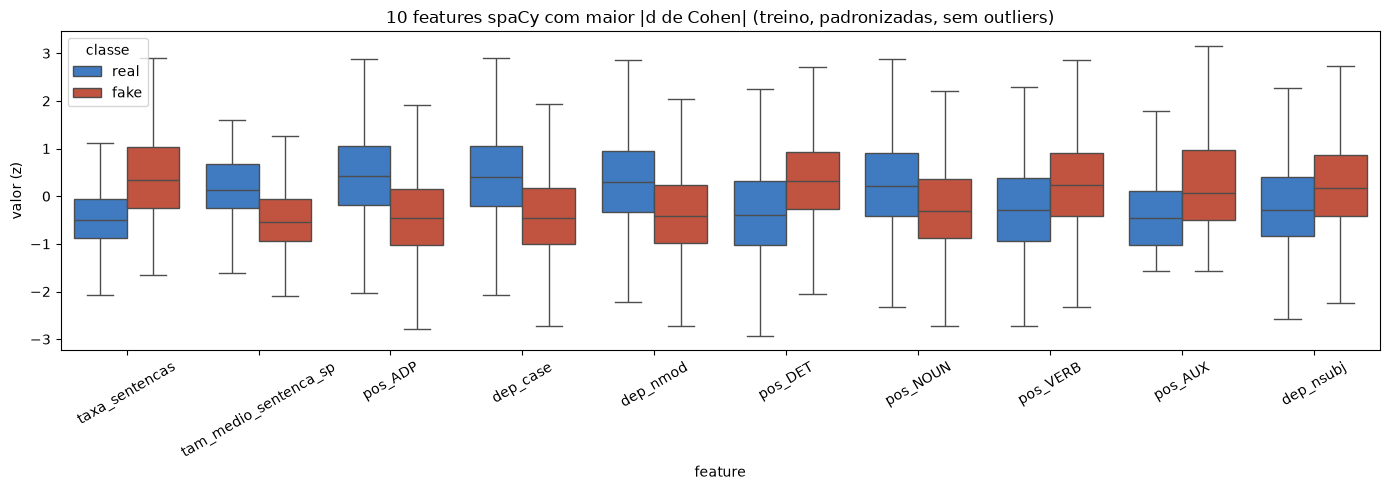
\includegraphics[width=0.95\linewidth,keepaspectratio]{entregavel-final-img/fig32.png}\\[2pt]{\small\emph{As 10 features spaCy com maior |d de Cohen| entre as classes (treino, padronizadas, sem outliers). Fonte: notebook 10\_svm\_metadados\_spacy.}}\end{center}

\begin{center}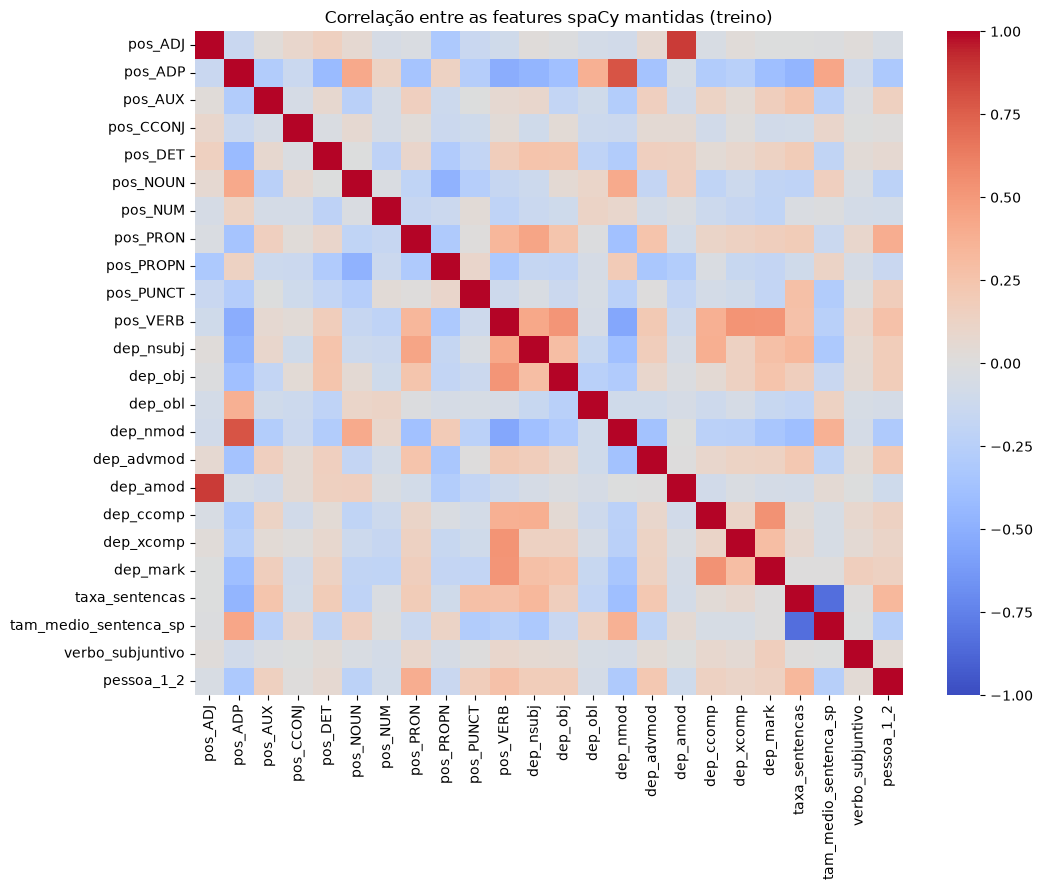
\includegraphics[width=0.75\linewidth,keepaspectratio]{entregavel-final-img/fig33.png}\\[2pt]{\small\emph{Correlação entre as features spaCy mantidas (treino). Fonte: notebook 10\_svm\_metadados\_spacy.}}\end{center}

\paragraph{Validação cruzada interna: ganho pequeno, só com peso baixo}\label{validauxe7uxe3o-cruzada-interna-ganho-pequeno-suxf3-com-peso-baixo}

{\def\LTcaptype{none} % do not increment counter
\begin{longtable}[]{@{}
  >{\raggedright\arraybackslash}p{(\linewidth - 16\tabcolsep) * \real{0.1111}}
  >{\raggedright\arraybackslash}p{(\linewidth - 16\tabcolsep) * \real{0.1111}}
  >{\raggedright\arraybackslash}p{(\linewidth - 16\tabcolsep) * \real{0.1111}}
  >{\raggedright\arraybackslash}p{(\linewidth - 16\tabcolsep) * \real{0.1111}}
  >{\raggedright\arraybackslash}p{(\linewidth - 16\tabcolsep) * \real{0.1111}}
  >{\raggedright\arraybackslash}p{(\linewidth - 16\tabcolsep) * \real{0.1111}}
  >{\raggedright\arraybackslash}p{(\linewidth - 16\tabcolsep) * \real{0.1111}}
  >{\raggedright\arraybackslash}p{(\linewidth - 16\tabcolsep) * \real{0.1111}}
  >{\raggedright\arraybackslash}p{(\linewidth - 16\tabcolsep) * \real{0.1111}}@{}}
\toprule\noalign{}
\begin{minipage}[b]{\linewidth}\raggedright
config
\end{minipage} & \begin{minipage}[b]{\linewidth}\raggedright
C
\end{minipage} & \begin{minipage}[b]{\linewidth}\raggedright
w
\end{minipage} & \begin{minipage}[b]{\linewidth}\raggedright
texto
\end{minipage} & \begin{minipage}[b]{\linewidth}\raggedright
F1 treino
\end{minipage} & \begin{minipage}[b]{\linewidth}\raggedright
F1 CV ± std
\end{minipage} & \begin{minipage}[b]{\linewidth}\raggedright
gap
\end{minipage} & \begin{minipage}[b]{\linewidth}\raggedright
Δ vs B0
\end{minipage} & \begin{minipage}[b]{\linewidth}\raggedright
folds melhores
\end{minipage} \\
\midrule\noalign{}
\endhead
\bottomrule\noalign{}
\endlastfoot
B0 & 1 & -- & -- & 1.0000 & 0.9295 ± 0.0099 & 0.0705 & -- & -- \\
M2 & 1 & 0,03 & todo o texto & 1.0000 & 0.9344 ± 0.0103 & 0.0656 & +0.0049 & 5/5 \\
M2 + χ² k=50 mil & 1 & 0,03 & 50 mil & 0.9999 & 0.9397 ± 0.0066 & 0.0601 & +0.0102 & 5/5 \\
M2 + χ² k=20 mil & 1 & 0,03 & 20 mil & 0.9952 & 0.9358 ± 0.0061 & 0.0595 & +0.0062 & 3/5 \\
S1 (só spaCy) & 0.1 & -- & 24 atributos & 0.7852 & 0.7824 ± 0.0082 & 0.0028 & -0.1471 & 0/5 \\
\end{longtable}
}

\begin{itemize}
\tightlist
\item
  \textbf{O peso importa.} Com w ≥ 0,3 o Δ é ≤ 0 em quase todo C; com C=0,1, qualquer w piora (até −0,021). O bloco denso, se não atenuado, toma a margem do TF-IDF. É consistente com a hipótese de escala, mas ela não foi testada na Regressão Logística, onde a piora tinha aparecido.
\item
  \textbf{O ganho é frágil.} Só a célula C=1, w=0,03 chega a 5/5 folds; as vizinhas ficam em 2--4/5. O ótimo está na borda do grid de w e é o máximo entre 25 candidatos (viés de seleção).
\item
  \textbf{χ² + spaCy.} Com k=50 mil o M2 chega a 0,9397, mas o mesmo χ² no B0 empatava (0,9288, notebook 08) e o número vem de duas rodadas de seleção, sem ter sido avaliado no teste.
\item
  \textbf{S1.} Há sinal (F1 0,78), mas modesto, com gap ≈ 0 por \emph{underfitting}.
\end{itemize}

\begin{center}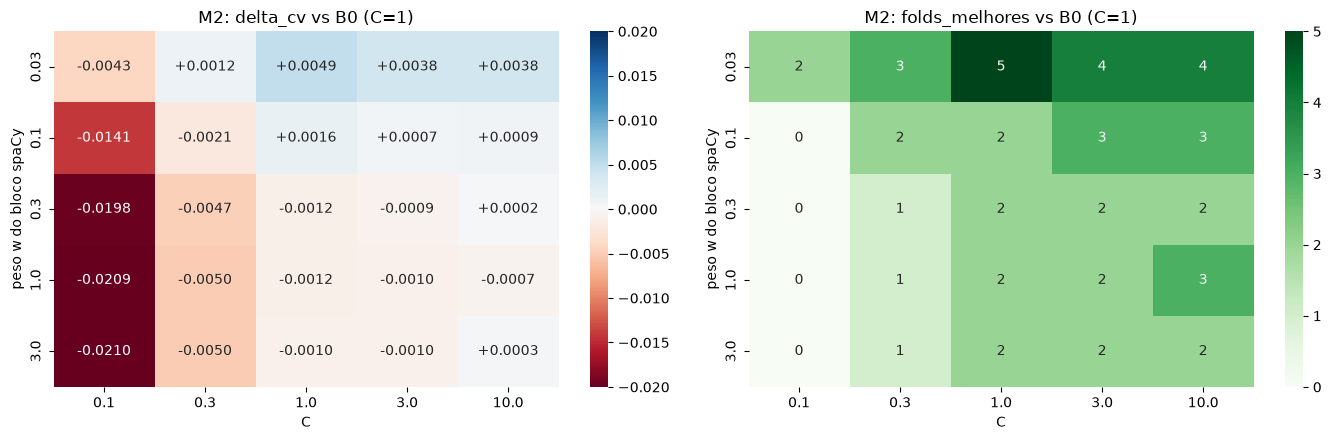
\includegraphics[width=0.95\linewidth,keepaspectratio]{entregavel-final-img/fig34.png}\\[2pt]{\small\emph{M2 vs B0 na CV: Δ F1 (esquerda) e número de folds melhores (direita) por C e peso w do bloco spaCy. Fonte: notebook 10\_svm\_metadados\_spacy.}}\end{center}

\begin{center}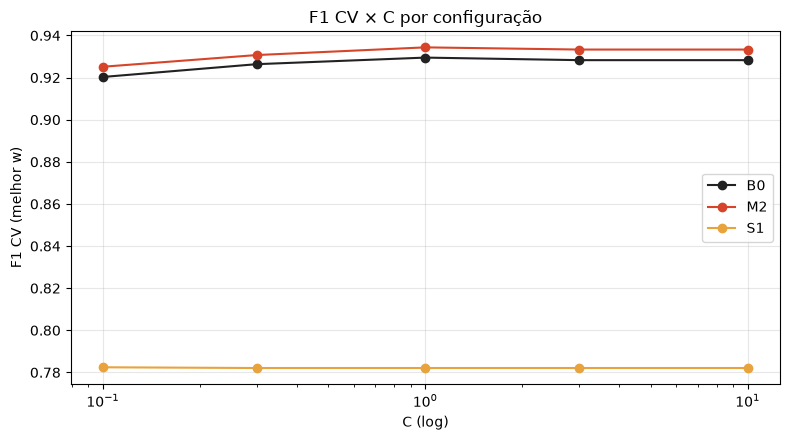
\includegraphics[width=0.7\linewidth,keepaspectratio]{entregavel-final-img/fig35.png}\\[2pt]{\small\emph{F1 CV × C por configuração (B0, M2, S1). Fonte: notebook 10\_svm\_metadados\_spacy.}}\end{center}

\paragraph{Teste interno e teste externo}\label{teste-interno-e-teste-externo}

{\def\LTcaptype{none} % do not increment counter
\begin{longtable}[]{@{}
  >{\raggedright\arraybackslash}p{(\linewidth - 12\tabcolsep) * \real{0.1429}}
  >{\raggedright\arraybackslash}p{(\linewidth - 12\tabcolsep) * \real{0.1429}}
  >{\raggedright\arraybackslash}p{(\linewidth - 12\tabcolsep) * \real{0.1429}}
  >{\raggedright\arraybackslash}p{(\linewidth - 12\tabcolsep) * \real{0.1429}}
  >{\raggedright\arraybackslash}p{(\linewidth - 12\tabcolsep) * \real{0.1429}}
  >{\raggedright\arraybackslash}p{(\linewidth - 12\tabcolsep) * \real{0.1429}}
  >{\raggedright\arraybackslash}p{(\linewidth - 12\tabcolsep) * \real{0.1429}}@{}}
\toprule\noalign{}
\begin{minipage}[b]{\linewidth}\raggedright
conjunto
\end{minipage} & \begin{minipage}[b]{\linewidth}\raggedright
modelo
\end{minipage} & \begin{minipage}[b]{\linewidth}\raggedright
F1 macro
\end{minipage} & \begin{minipage}[b]{\linewidth}\raggedright
ROC-AUC
\end{minipage} & \begin{minipage}[b]{\linewidth}\raggedright
\% previsto fake
\end{minipage} & \begin{minipage}[b]{\linewidth}\raggedright
falsos positivos
\end{minipage} & \begin{minipage}[b]{\linewidth}\raggedright
falsos negativos
\end{minipage} \\
\midrule\noalign{}
\endhead
\bottomrule\noalign{}
\endlastfoot
interno (Fake.br) & B0 & 0.9222 & 0.9830 & 49.7\% & 54 & 58 \\
interno (Fake.br) & M2 & 0.9236 & 0.9846 & 49.6\% & 52 & 58 \\
externo (FakeRecogna, títulos) & B0 & 0.6119 & 0.7072 & 70.8\% & 1438 & 407 \\
externo (FakeRecogna, títulos) & M2 & 0.6134 & 0.6622 & 59.3\% & 1184 & 720 \\
externo (FakeRecogna, títulos) & S1 & 0.5577 & 0.5845 & 57.9\% & 1287 & 897 \\
\end{longtable}
}

\begin{itemize}
\tightlist
\item
  \textbf{Interno:} a direção é a da CV, mas +0,0014 de F1 está dentro do erro padrão (\textasciitilde±0,007 com 1.440 notícias).
\item
  \textbf{Externo:} o spaCy desloca o limiar (menos "fake") mas \textbf{ordena pior}: o AUC cai de 0,707 para 0,662. Os títulos têm mediana de 13 tokens contra 114 no treino, e \texttt{taxa\_sentencas} e \texttt{tam\_medio\_sentenca}, as features de maior peso, saem da distribuição vista no treino. Isso é um risco direto para o app, que receberá textos de tamanhos e formatos variados.
\end{itemize}

\begin{center}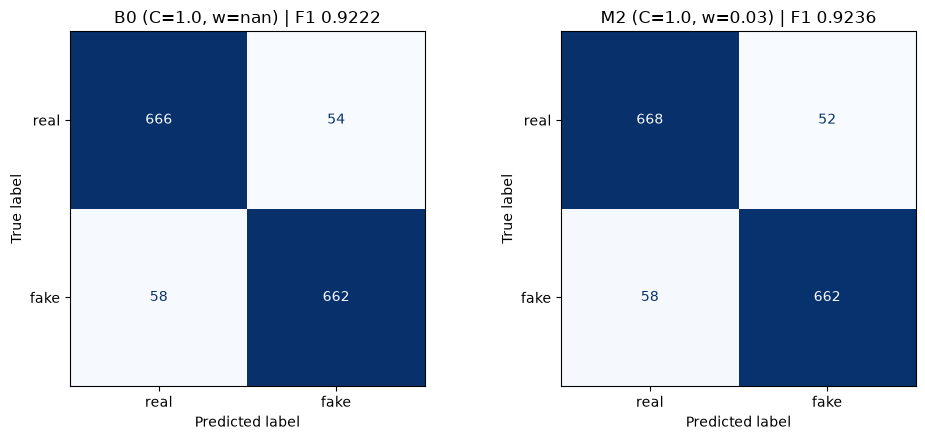
\includegraphics[width=0.85\linewidth,keepaspectratio]{entregavel-final-img/fig36.png}\\[2pt]{\small\emph{Matrizes de confusão no teste interno: B0 (esquerda) e M2 (direita). Fonte: notebook 10\_svm\_metadados\_spacy.}}\end{center}

\begin{center}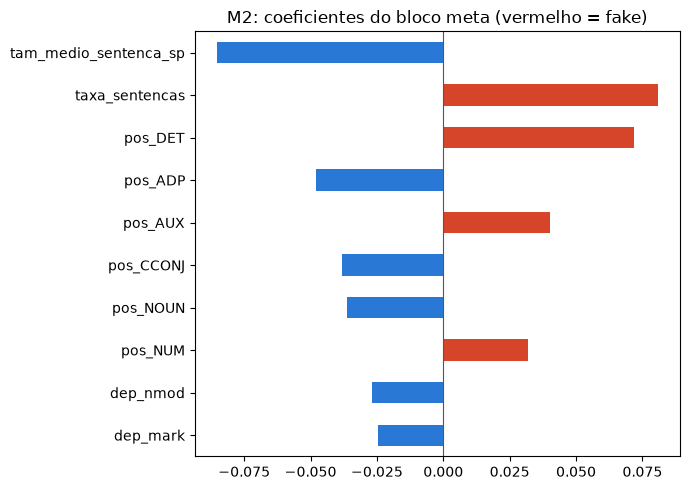
\includegraphics[width=0.6\linewidth,keepaspectratio]{entregavel-final-img/fig37.png}\\[2pt]{\small\emph{Coeficientes do bloco de metadados spaCy no M2 (vermelho = fake). Fonte: notebook 10\_svm\_metadados\_spacy.}}\end{center}

\begin{quote}
\textbf{{[}NOTA{]}} O desfecho difere do que o grid search sugeria (metadados ajudando, 0,9415 em 3 folds). Aqui, no bloco spaCy, o ganho é de +0,005 na CV, sem ganho comprovado no teste interno e com perda de generalização externa.
\end{quote}

\subsection{5.7 Interpretabilidade (SHAP)}\label{interpretabilidade-shap}

Para a análise de importância das variáveis, a técnica SHAP \emph{(SHapley Additive exPlanations}) se integra à arquitetura do projeto por sua capacidade de avaliar os parâmetros não de forma isolada, mas sim como eles atuam em conjunto. Baseado na Teoria dos Jogos, esse método permite ao sistema compreender a complementaridade matemática entre as variáveis, interpretando cenários complexos onde a presença de uma fonte reconhecida precisa estar necessariamente aliada a um contexto ou bibliografia consistente para atestar a confiabilidade da notícia. Como algoritmos baseados em árvores de decisão conseguem aprender essas regras condicionais de forma orgânica, o SHAP interpreta as predições do modelo e gera uma matriz de interação que mede a força exata da união dessas variáveis. Isso contorna as limitações de outras técnicas explicativas diante de parâmetros altamente correlacionados, como o excesso de emoção e o uso de verbos no imperativo. Ou seja, o fluxo consiste em treinar o modelo de classificação com o dataset, processar a notícia pelo explicador do SHAP e extrair os atributos de maior impacto para aquele veredito específico. Esses ofensores matemáticos são então filtrados e enviados como contexto para o modelo socrático gerar a pergunta reflexiva correspondente, garantindo que o alerta exibido no sistema de semáforo possua uma justificativa rastreável e diretamente baseada na estrutura da notícia.

\textbf{Beeswarm plot.} O gráfico de \emph{beeswarm plot} exibe o impacto e a direção de cada atributo na predição de notícias falsas, ordenando as variáveis por importância no eixo vertical. No eixo horizontal, os valores SHAP positivos indicam que o indicador empurra o veredito para a desinformação, enquanto os negativos apontam para a autenticidade, com a escala de cores representando o valor real de cada métrica (do azul para valores baixos ao rosa para valores altos). O resultado demonstra que a \textbf{diversidade} lidera o impacto preditivo, tal qual o boxplot representou, evidenciando de forma direta como intensidades específicas de cada variável linguística moldam a decisão do modelo e sustentam as intervenções analíticas do sistema.

\subsubsection{Desenvolvimento}\label{desenvolvimento}

A implementação do cálculo de interações globais via SHAP expande a interpretação para além dos atributos isolados, mapeando como o modelo de aprendizado de máquina cruza duplas de variáveis para fundamentar suas predições. O procedimento inicia-se com a extração da matriz tridimensional de interações, que passa por um tratamento de dimensionalidade para isolar especificamente a classe de interesse voltada às notícias falsas. A partir disso, o sistema calcula a média dos valores absolutos dessa matriz em todo o conjunto de teste, condensando a complexidade estatística em uma métrica objetiva que quantifica a força de sinergia entre cada par de características textuais.

Para estruturar o resultado, o código varre o conjunto de atributos de maneira combinatória, ignorando comparações repetidas e a identidade própria das variáveis, a fim de consolidar os dados em um ranking ordenado de forma decrescente. Esse arranjo exibe as combinações mais potentes identificadas pelo algoritmo, destacando no topo duplas como a \textbf{taxa\_verbos\_subj\_imp} combinada com a \textbf{diversidade}. Essa visão matricial comprova que o classificador opera por meio de regras lógicas conjuntas, fornecendo a base analítica essencial para que o sistema compreenda a dinâmica estrutural da desinformação e fundamente suas intervenções socráticas na interface.

\subsubsection{Visualização}\label{visualizauxe7uxe3o}

O gráfico de dispersão bivariado ilustra a interação entre as duas variáveis mais importantes \textbf{taxa\_verbos\_subj\_imp} e \textbf{diversidade}, posicionando no eixo horizontal e eixo vertical, onde o impacto marginal corresponde o veredito de desinformação. A escala de cores lateral representa o nível de \textbf{diversidade} de cada instância, permitindo observar diretamente como essa segunda variável modula e altera o comportamento da primeira. Os pontos demonstram que o peso preditivo atribuído aos verbos modais e imperativos varia conforme o contexto da riqueza de vocabulário do texto, fornecendo a evidência visual da sinergia entre os fatores estruturais e fundamentando a lógica complexa que sustenta as intervenções analíticas da plataforma.

\begin{quote}
\textbf{{[}NOTA{]}} O gráfico de interação aponta \texttt{taxa\_verbos\_subj\_imp} (verbos no \textbf{subjuntivo ou imperativo}; o texto original dizia "modais e imperativos") e \texttt{diversidade} como o par mais forte. Os notebooks de origem (SHAP de interação e \emph{beeswarm}) não estão versionados e o modelo escolhido (LinearSVC sobre TF-IDF) não tem SHAP implementado.
\end{quote}

Complementarmente, o notebook \texttt{02\_LR\_training} traz gráficos \emph{beeswarm} do SHAP (\texttt{LinearExplainer}) calculados sobre a Regressão Logística com TF-IDF, que mostram as palavras de maior impacto na decisão:

\begin{center}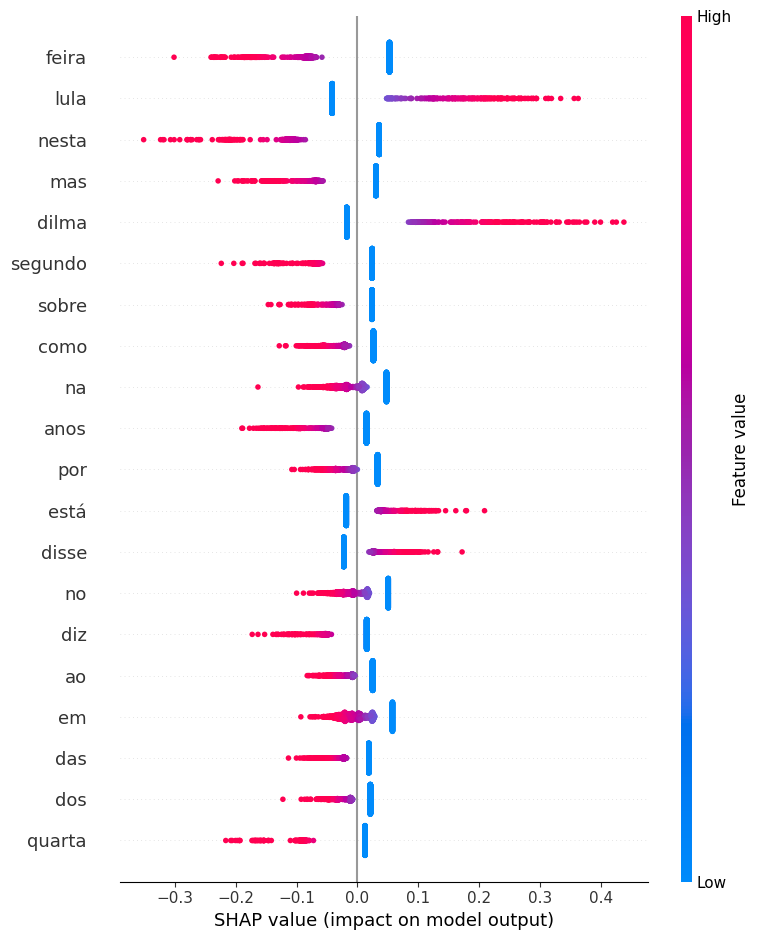
\includegraphics[width=0.65\linewidth,keepaspectratio]{entregavel-final-img/fig27.png}\\[2pt]{\small\emph{SHAP summary plot: 20 termos de maior impacto (Regressão Logística). Fonte: notebook 02\_LR\_training.}}\end{center}

\begin{center}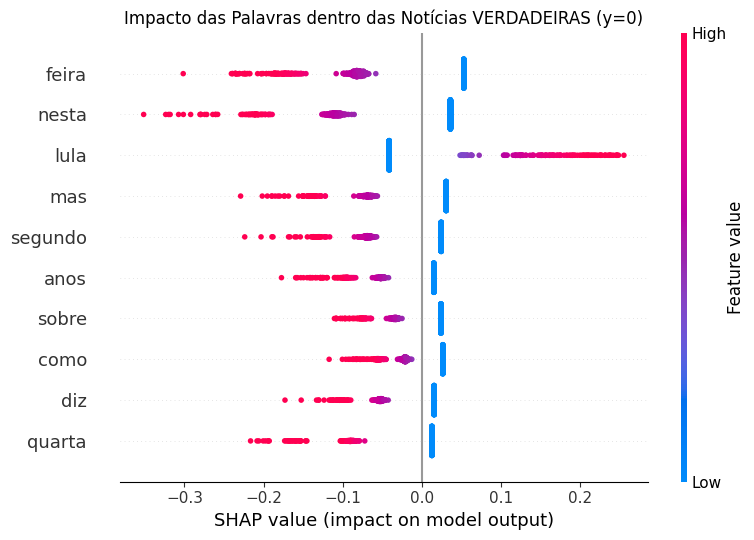
\includegraphics[width=0.7\linewidth,keepaspectratio]{entregavel-final-img/fig28.png}\\[2pt]{\small\emph{SHAP: impacto das palavras nas notícias verdadeiras (y=0). Fonte: notebook 02\_LR\_training.}}\end{center}

\begin{center}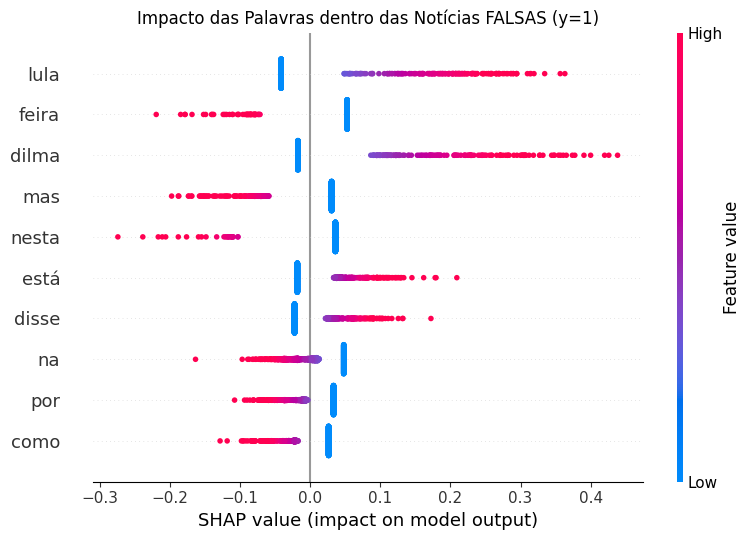
\includegraphics[width=0.7\linewidth,keepaspectratio]{entregavel-final-img/fig29.png}\\[2pt]{\small\emph{SHAP: impacto das palavras nas notícias falsas (y=1). Fonte: notebook 02\_LR\_training.}}\end{center}

\begin{quote}
\textbf{{[}PENDENTE{]}} Versionar o notebook do SHAP (o gráfico acima vem de um notebook externo). No modelo de produção a explicação não depende de SHAP: o score se decompõe exatamente em contribuições por n-grama e por atributo spaCy (seção 5.11).
\end{quote}

\subsection{5.8 Dimensionalidade e kernels}\label{dimensionalidade-e-kernels}

\subsubsection{\texorpdfstring{Redução de dimensionalidade (\texttt{08\_reducao\_dim}, \texttt{05})}{Redução de dimensionalidade (08\_reducao\_dim, 05)}}\label{reduuxe7uxe3o-de-dimensionalidade-08_reducao_dim-05}

Pergunta: reduzir o número de atributos (\textasciitilde114 mil para \textasciitilde5,7 mil documentos) melhora o F1 ou diminui o gap? Todas as reduções são ajustadas dentro do \texttt{Pipeline}, no treino de cada fold. O \texttt{PCA} do scikit-learn não aceita matriz esparsa (centralizá-la a tornaria densa, \textasciitilde5,3 GB), então usa-se \textbf{TruncatedSVD (LSA)} com \texttt{Normalizer}. Técnicas comparadas: poda por \texttt{min\_df}, TruncatedSVD (d de 2 a 300), seleção univariada χ² (\texttt{SelectKBest}, k de 500 a 80.000) e seleção por modelo com penalidade L1 (\texttt{SelectFromModel}).

{\def\LTcaptype{none} % do not increment counter
\begin{longtable}[]{@{}llllll@{}}
\toprule\noalign{}
método & features & F1 CV & Δ vs base & gap & folds melhores \\
\midrule\noalign{}
\endhead
\bottomrule\noalign{}
\endlastfoot
base & 114.301 & 0.9295 & +0.0000 & 0.0705 & 0 \\
chi2 (k=80000) & 80.000 & 0.9291 & -0.0004 & 0.0700 & 2 \\
chi2 (k=50000) & 50.000 & 0.9288 & -0.0007 & 0.0676 & 2 \\
chi2 (k=20000) & 20.000 & 0.9241 & -0.0054 & 0.0601 & 1 \\
chi2 (k=10000) & 10.000 & 0.9189 & -0.0106 & 0.0509 & 1 \\
chi2 (k=2000) & 2.000 & 0.8951 & -0.0344 & 0.0297 & 0 \\
l1 (C=1) & 7.854 & 0.9214 & -0.0081 & 0.0668 & 1 \\
svd (pca) (d=300) & 300 & 0.9062 & -0.0233 & 0.0326 & 0 \\
svd (pca) (d=50) & 50 & 0.8663 & -0.0632 & 0.0059 & 0 \\
svd (pca) (d=10) & 10 & 0.7812 & -0.1483 & -0.0013 & 0 \\
svd (pca) (d=2) & 2 & 0.5482 & -0.3813 & -0.0001 & 0 \\
\end{longtable}
}

\begin{itemize}
\tightlist
\item
  \textbf{Nenhuma técnica superou a baseline} na validação cruzada. O desvio do F1 é \textasciitilde0,010, então χ² com k ≥ 50.000 empata com ela.
\item
  \textbf{O gap só se aproxima de zero com \emph{underfitting}}: com SVD d ≤ 20 o F1 é baixo e o gap ≈ 0. Gap baixo aqui significa que o modelo não ajusta nem o treino.
\item
  \textbf{Com o mesmo orçamento de atributos, χ² supera SVD}: com k=2.000 já bate o SVD de 100 componentes (0,8951 contra 0,8838). Os n-gramas específicos carregam o sinal e a projeção densa o dilui.
\item
  \textbf{Visualização 2D} (d=2): as duas componentes explicam \textasciitilde0,75\% da variância, captam padrões genéricos (tamanho, palavras funcionais) e misturam as classes; o F1 de \textasciitilde0,55 é praticamente o acaso.
\item
  \textbf{Conclusão}: para texto, o regime esparso com d ≫ N é favorável a modelos lineares; reduzir demais descarta informação útil. Se for reduzir, preferir seleção supervisionada (χ²).
\end{itemize}

\subsubsection{\texorpdfstring{Kernels não lineares (\texttt{09\_kernels\_svm})}{Kernels não lineares (09\_kernels\_svm)}}\label{kernels-nuxe3o-lineares-09_kernels_svm}

Hipótese: um kernel RBF ou polinomial valeria mais que o LinearSVC? Pelo teorema de Cover o espaço de \textasciitilde114 mil dimensões já é praticamente linearmente separável, e o \texttt{SVC} com kernel exige matriz de Gram (memória O(n²)), muito mais custosa que o \texttt{liblinear}. O notebook conclui que o LinearSVC é equivalente ou superior em F1 e muito mais barato.

\subsubsection{Redução de dimensão no modelo com spaCy (notebooks 11 e 12)}\label{reduuxe7uxe3o-de-dimensuxe3o-no-modelo-com-spacy-notebooks-11-e-12}

Repetida a pergunta com o M2 (C=1, w=0,03 fixos). Primeiro, \texttt{TruncatedSVD(d)} + \texttt{Normalizer} no bloco de texto (o bloco spaCy não é reduzido):

{\def\LTcaptype{none} % do not increment counter
\begin{longtable}[]{@{}
  >{\raggedright\arraybackslash}p{(\linewidth - 10\tabcolsep) * \real{0.1667}}
  >{\raggedright\arraybackslash}p{(\linewidth - 10\tabcolsep) * \real{0.1667}}
  >{\raggedright\arraybackslash}p{(\linewidth - 10\tabcolsep) * \real{0.1667}}
  >{\raggedright\arraybackslash}p{(\linewidth - 10\tabcolsep) * \real{0.1667}}
  >{\raggedright\arraybackslash}p{(\linewidth - 10\tabcolsep) * \real{0.1667}}
  >{\raggedright\arraybackslash}p{(\linewidth - 10\tabcolsep) * \real{0.1667}}@{}}
\toprule\noalign{}
\begin{minipage}[b]{\linewidth}\raggedright
d (texto)
\end{minipage} & \begin{minipage}[b]{\linewidth}\raggedright
F1 treino (M2)
\end{minipage} & \begin{minipage}[b]{\linewidth}\raggedright
F1 CV (M2)
\end{minipage} & \begin{minipage}[b]{\linewidth}\raggedright
gap (M2)
\end{minipage} & \begin{minipage}[b]{\linewidth}\raggedright
Δ vs M2 completo
\end{minipage} & \begin{minipage}[b]{\linewidth}\raggedright
ganho do spaCy (M2 − B0)
\end{minipage} \\
\midrule\noalign{}
\endhead
\bottomrule\noalign{}
\endlastfoot
completo & 1.0000 & 0.9344 & 0.0656 & -- & +0.0049 \\
500 & 0.9580 & 0.9218 & 0.0361 & -0.0125 (0/5) & +0.0067 \\
300 & 0.9454 & 0.9212 & 0.0242 & -0.0132 (0/5) & +0.0134 \\
100 & 0.9111 & 0.9000 & 0.0111 & -0.0344 (0/5) & +0.0162 \\
50 & 0.8991 & 0.8894 & 0.0097 & -0.0450 (0/5) & +0.0231 \\
\end{longtable}
}

\textbf{O gap cai porque o treino piora, não porque a validação melhora}: o F1 CV perde em todo d e em todos os folds, e nenhum d é escolhido pela regra fixada antes de rodar (menor gap com Δ ≥ −0,01). O spaCy pesa mais com o texto comprimido (+0,023 com d=50), mas nenhum M2 reduzido alcança o texto completo. O SVD só foi até d=500, por limite de memória.

\begin{center}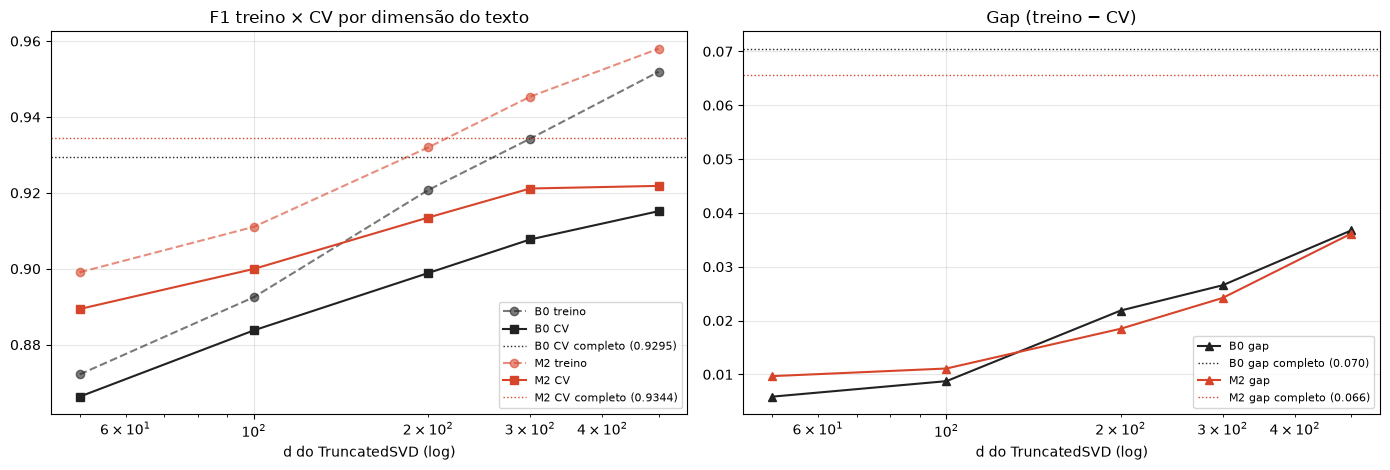
\includegraphics[width=0.95\linewidth,keepaspectratio]{entregavel-final-img/fig38.png}\\[2pt]{\small\emph{SVD no modelo M2: F1 de treino e CV por dimensão d (esquerda) e gap (direita). Fonte: notebook 11\_reducao\_dim\_svm\_spacy.}}\end{center}

\begin{center}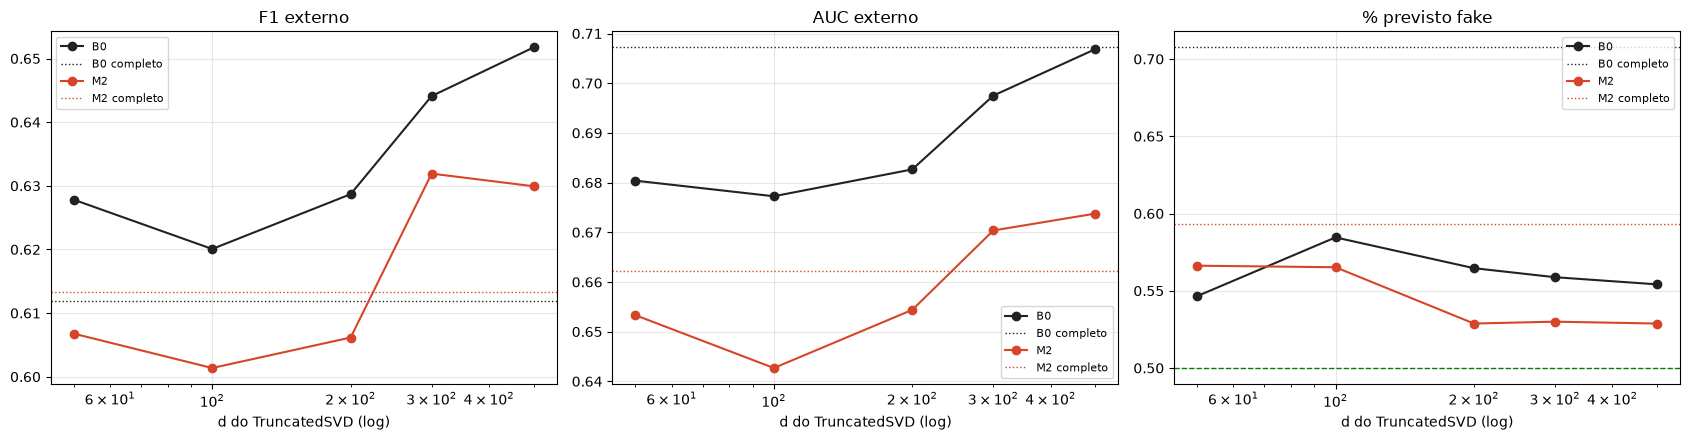
\includegraphics[width=0.95\linewidth,keepaspectratio]{entregavel-final-img/fig39.png}\\[2pt]{\small\emph{SVD no modelo M2: desempenho externo (FakeRecogna) por dimensão d. Fonte: notebook 11\_reducao\_dim\_svm\_spacy.}}\end{center}

Depois, \texttt{TF-IDF\ →\ SelectKBest(χ²,\ k)\ →\ TruncatedSVD(500)\ →\ Normalizer}, ajustado por fold, variando só k:

{\def\LTcaptype{none} % do not increment counter
\begin{longtable}[]{@{}
  >{\raggedright\arraybackslash}p{(\linewidth - 12\tabcolsep) * \real{0.1429}}
  >{\raggedright\arraybackslash}p{(\linewidth - 12\tabcolsep) * \real{0.1429}}
  >{\raggedright\arraybackslash}p{(\linewidth - 12\tabcolsep) * \real{0.1429}}
  >{\raggedright\arraybackslash}p{(\linewidth - 12\tabcolsep) * \real{0.1429}}
  >{\raggedright\arraybackslash}p{(\linewidth - 12\tabcolsep) * \real{0.1429}}
  >{\raggedright\arraybackslash}p{(\linewidth - 12\tabcolsep) * \real{0.1429}}
  >{\raggedright\arraybackslash}p{(\linewidth - 12\tabcolsep) * \real{0.1429}}@{}}
\toprule\noalign{}
\begin{minipage}[b]{\linewidth}\raggedright
texto
\end{minipage} & \begin{minipage}[b]{\linewidth}\raggedright
F1 treino
\end{minipage} & \begin{minipage}[b]{\linewidth}\raggedright
F1 CV (M2)
\end{minipage} & \begin{minipage}[b]{\linewidth}\raggedright
gap
\end{minipage} & \begin{minipage}[b]{\linewidth}\raggedright
Δ vs M2 completo
\end{minipage} & \begin{minipage}[b]{\linewidth}\raggedright
ganho do spaCy
\end{minipage} & \begin{minipage}[b]{\linewidth}\raggedright
AUC externo (M2 / B0)
\end{minipage} \\
\midrule\noalign{}
\endhead
\bottomrule\noalign{}
\endlastfoot
completo & 1.0000 & 0.9344 & 0.0656 & -- & +0.0049 & 0.662 / 0.707 \\
SVD500 sem χ² & 0.9580 & 0.9218 & 0.0361 & -0.0125 (0/5) & +0.0067 & 0.674 / 0.707 \\
χ² 1 mil + SVD500 & 0.9601 & 0.9189 & 0.0412 & -0.0154 (0/5) & +0.0135 & 0.649 / 0.657 \\
χ² 5 mil + SVD500 & 0.9698 & 0.9266 & 0.0433 & -0.0078 (1/5) & +0.0097 & 0.662 / 0.664 \\
χ² 10 mil + SVD500 & 0.9717 & 0.9295 & 0.0422 & -0.0049 (1/5) & +0.0097 & 0.677 / 0.686 \\
χ² 20 mil + SVD500 & 0.9741 & 0.9300 & 0.0441 & -0.0043 (0/5) & +0.0073 & 0.681 / 0.685 \\
χ² 50 mil + SVD500 & 0.9724 & 0.9293 & 0.0431 & -0.0050 (2/5) & +0.0043 & 0.684 / 0.691 \\
\end{longtable}
}

\begin{center}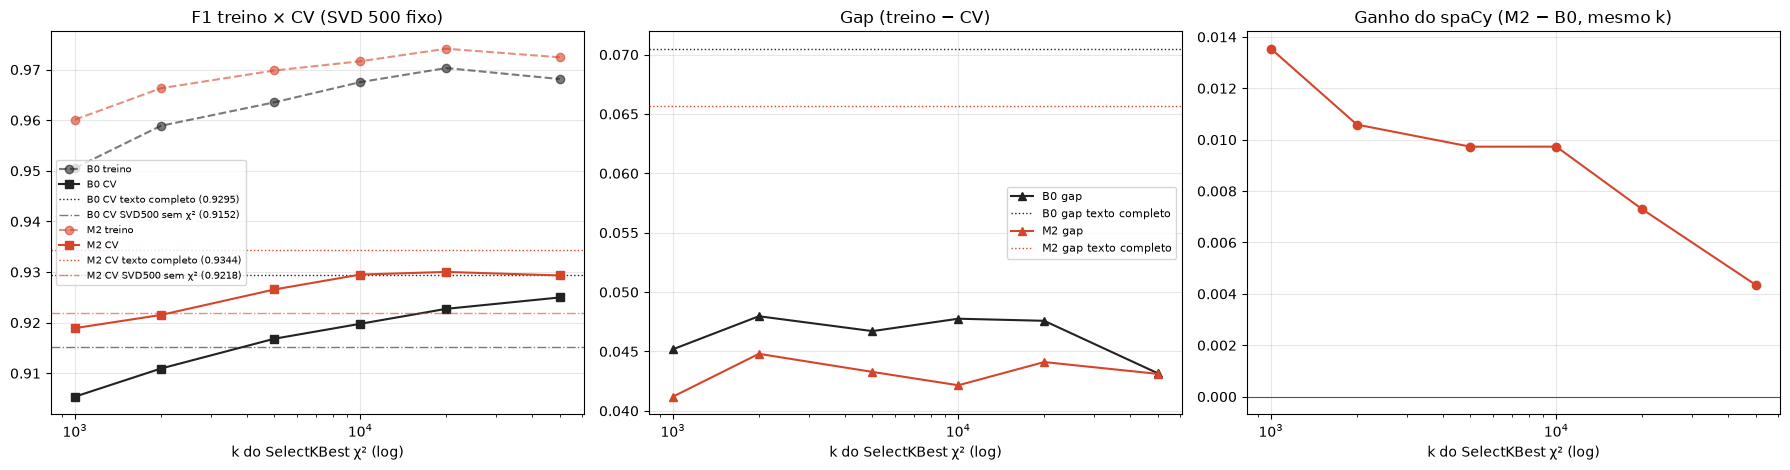
\includegraphics[width=0.95\linewidth,keepaspectratio]{entregavel-final-img/fig40.png}\\[2pt]{\small\emph{M2 com SelectKBest χ² + SVD(500): F1 treino/CV, gap e ganho do spaCy por k. Fonte: notebook 12\_selectk\_svd\_svm\_spacy.}}\end{center}

\begin{itemize}
\tightlist
\item
  \textbf{O χ² recupera o que o SVD sozinho perdia.} Com k=10--50 mil o M2 fica em \textasciitilde0,930, o mesmo F1 CV do SVM atual (0,9295), e o gap cai de 0,0705 para \textasciitilde0,043. Diferente do SVD sozinho, o gap cai \textbf{sem} a validação cair frente ao B0.
\item
  \textbf{Escolha pela regra do notebook 11: k = 10 mil} (F1 CV 0,9295 ± 0,0081, gap 0,042). É empate, não vitória: perde para o M2 completo em 4/5 folds. O spaCy contribui o dobro nesse regime (+0,010 contra +0,005).
\item
  \textbf{Teste interno} do M2 com χ² 10 mil + SVD(500): F1 0,9243 e AUC 0,9789, contra 0,9236 e 0,9846 do M2 completo e 0,9222 e 0,9830 do B0, tudo dentro do ruído.
\item
  \textbf{Fora do domínio (espiada):} o χ² \textbf{piora a ordenação}; o AUC do B0 cai de 0,707 para ≤ 0,691 e o do M2 com k=10 mil fica em 0,677, porque o χ² escolhe os n-gramas que separam o Fake.br e especializa o modelo no corpus.
\end{itemize}

\begin{center}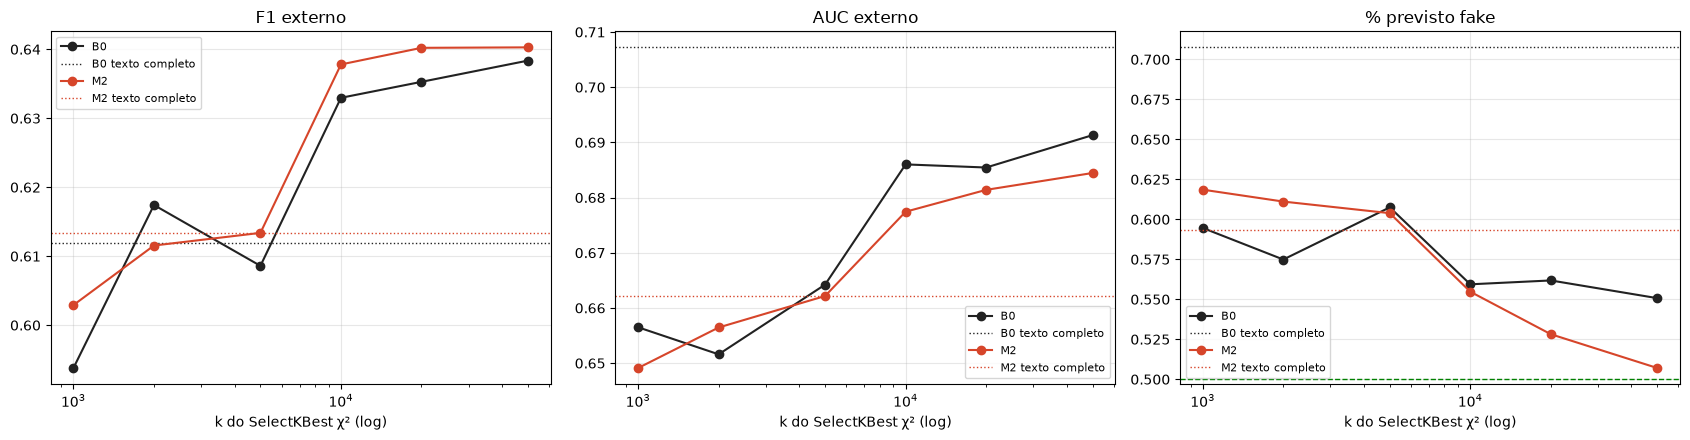
\includegraphics[width=0.95\linewidth,keepaspectratio]{entregavel-final-img/fig41.png}\\[2pt]{\small\emph{SelectKBest χ² + SVD(500): desempenho externo (FakeRecogna) por k. Fonte: notebook 12\_selectk\_svd\_svm\_spacy.}}\end{center}

\begin{quote}
\textbf{{[}NOTA{]}} Pela regra "melhor média de CV", a configuração escolhida seria M2 + χ² k=50 mil (0,9397), mas o teste avaliou o M2 com todo o texto, e o χ² foi aplicado depois de escolher C e w, então essa estimativa é otimista. As avaliações externas são "espiadas" (uma vez, sem intervalo de confiança).
\end{quote}

\begin{quote}
\textbf{{[}PENDENTE{]}} O notebook \texttt{09} não tem outputs salvos e \texttt{resultados\_kernels.csv} não existe no repositório; a conclusão acima está escrita no notebook, mas sem evidência numérica versionada. Executar e commitar o CSV.
\end{quote}

\subsection{5.9 Generalização fora do corpus (teste externo no FakeRecogna)}\label{generalizauxe7uxe3o-fora-do-corpus-teste-externo-no-fakerecogna}

Treino no Fake.br, avaliação em títulos do FakeRecogna (seção 3.3), sem novo ajuste.

{\def\LTcaptype{none} % do not increment counter
\begin{longtable}[]{@{}lllll@{}}
\toprule\noalign{}
modelo & n\_dim & f1\_externo & auc\_externo & pct\_prev\_fake \\
\midrule\noalign{}
\endhead
\bottomrule\noalign{}
\endlastfoot
Base (word+char) & 114301 & 0.6122 & 0.7072 & 70.7\% \\
PCA/SVD d=2 & 2 & 0.4004 & 0.4822 & 89.1\% \\
PCA/SVD d=5 & 5 & 0.5799 & 0.6238 & 66.8\% \\
PCA/SVD d=10 & 10 & 0.6005 & 0.6412 & 48.4\% \\
PCA/SVD d=20 & 20 & 0.6166 & 0.6622 & 46.3\% \\
PCA/SVD d=50 & 50 & 0.6278 & 0.6804 & 54.6\% \\
PCA/SVD d=100 & 100 & 0.6201 & 0.6773 & 58.5\% \\
PCA/SVD d=200 & 200 & 0.6287 & 0.6827 & 56.5\% \\
PCA/SVD d=300 & 300 & 0.6439 & 0.6975 & 55.9\% \\
PCA/SVD d=500 & 500 & 0.6518 & 0.7069 & 55.4\% \\
Chi2 k=5000 & 5000 & 0.6347 & 0.6976 & 60.0\% \\
Chi2 k=10000 & 10000 & 0.6448 & 0.7101 & 57.8\% \\
Chi2 k=20000 & 20000 & 0.6451 & 0.7115 & 60.2\% \\
Chi2 k=50000 & 50000 & 0.6364 & 0.7110 & 63.4\% \\
Chi2 k=80000 & 80000 & 0.6231 & 0.7132 & 69.5\% \\
\end{longtable}
}

\begin{itemize}
\tightlist
\item
  \textbf{O F1 interno não se mantém}: de \textasciitilde0,93 para \textbf{0,6122} (AUC 0,7072), e o modelo prevê "fake" em \textbf{70,7\%} dos casos, o que indica viés de domínio.
\item
  Uma redução moderada (SVD d=300--500 ou χ² k=10--20 mil) sobe o F1 externo em \textasciitilde0,03--0,04 e aproxima a proporção prevista de fake de 50\%. \textbf{O AUC quase não muda (\textasciitilde0,70--0,71)}: grande parte do ganho vem de um limiar menos enviesado, não de uma ordenação melhor. O ganho é real, porém modesto.
\item
  Variar \texttt{min\_df} e C no teste externo também mexe pouco (F1 0,61--0,62 para \texttt{min\_df}; C baixo piora por enviesar para fake). SVD com d ≤ 5 fica no nível do acaso.
\item
  \textbf{O gargalo é o viés de domínio} entre Fake.br e FakeRecogna, que a redução de dimensionalidade não resolve. Os metadados spaCy (seção 5.6) e o χ² (seção 5.8) também não resolvem e, por ordenarem pior, reduzem o AUC externo.
\end{itemize}

Ressalvas: cada configuração externa foi avaliada uma única vez, sem intervalo de confiança; o conjunto externo é de títulos (mediana de 13 palavras) contra textos de 100 palavras no treino; e o SVD só foi avaliado até d=300 na validação interna (d=500 aparece apenas no externo).

\begin{quote}
\textbf{{[}NOTA{]}} O notebook \texttt{07} afirma que a redução "generaliza muito melhor". A formulação defensável é a deste documento (ganho modesto, AUC praticamente igual).
\end{quote}

\subsection{5.10 Validação, curva de aprendizado e dependência de convenções}\label{validauxe7uxe3o-curva-de-aprendizado-e-dependuxeancia-de-convenuxe7uxf5es}

\subsubsection{Dados de treino, validação e teste}\label{dados-de-treino-validauxe7uxe3o-e-teste}

Para treino, utilizamos 80\% do dataset tratado, separados com random\_state=42. Todos os experimentos de comparação entre configurações de features foram avaliados por validação cruzada (k-fold, k=5) sobre esse conjunto de treino, ou seja, cada fold representa 16\% do dataset total, 80\% do dataset dividido em 5 partes iguais. Em cada uma das 5 iterações, 4 folds são usados para treinar o modelo, equivalente a 64\%, e o fold restante é usado para validação, 16\% do dataset. Alternando qual fold desempenha esse papel a cada passada, garantindo que cada amostra de treino seja validada exatamente uma vez ao longo do processo.

Testamos e comparamos o uso de metadados estilométricos para o treinamento do modelo contra o uso apenas do texto truncado em 100 palavras e vetorizado via TF-IDF. A métrica de referência até agora foi obtida com os vetores de TF-IDF aplicado ao texto truncado (unigramas e bigramas de palavras) combinado ao TF-IDF aplicado a caracteres (trigramas a quinquigramas).

Optamos por não seguir com a pipeline de extração de metadados estilométricos como bloco principal: o ganho de acurácia que ela adiciona é pequeno frente ao esforço de engenharia necessário para extraí-la e validá-la, especialmente quando comparado ao ganho trazido pelos n-gramas de caractere.

\textbf{Validação.} Não há conjunto de validação fixo: a validação durante o treino é a validação cruzada acima. \textbf{Teste.} 20\% do dataset (1.440 textos), separados com \texttt{random\_state=42}, mantidos fora do treino, da validação cruzada e da seleção de configurações, com a mesma normalização e truncamento do treino. Cada modelo é avaliado uma única vez sobre ele.

Notebook de preparação e separação (necessário para rodar os demais): \url{https://colab.research.google.com/drive/1mW8e7tKF_w-ntmOOpB3vcUxF74CKMToh?usp=sharing}

\subsubsection{\texorpdfstring{Hold-out versus K-Fold (\texttt{03\_SVM\_training})}{Hold-out versus K-Fold (03\_SVM\_training)}}\label{hold-out-versus-k-fold-03_svm_training}

O notebook compara a validação por K-Fold e por Hold-out (80/20 do treino) e justifica k=5 testando k ∈ \{2, 3, 5, 10, 20\}, cada um repetido 5 vezes (config. word, LinearSVC):

{\def\LTcaptype{none} % do not increment counter
\begin{longtable}[]{@{}
  >{\raggedright\arraybackslash}p{(\linewidth - 12\tabcolsep) * \real{0.1429}}
  >{\raggedright\arraybackslash}p{(\linewidth - 12\tabcolsep) * \real{0.1429}}
  >{\raggedright\arraybackslash}p{(\linewidth - 12\tabcolsep) * \real{0.1429}}
  >{\raggedright\arraybackslash}p{(\linewidth - 12\tabcolsep) * \real{0.1429}}
  >{\raggedright\arraybackslash}p{(\linewidth - 12\tabcolsep) * \real{0.1429}}
  >{\raggedright\arraybackslash}p{(\linewidth - 12\tabcolsep) * \real{0.1429}}
  >{\raggedright\arraybackslash}p{(\linewidth - 12\tabcolsep) * \real{0.1429}}@{}}
\toprule\noalign{}
\begin{minipage}[b]{\linewidth}\raggedright
k
\end{minipage} & \begin{minipage}[b]{\linewidth}\raggedright
treino/fold
\end{minipage} & \begin{minipage}[b]{\linewidth}\raggedright
validação/fold
\end{minipage} & \begin{minipage}[b]{\linewidth}\raggedright
F1 médio
\end{minipage} & \begin{minipage}[b]{\linewidth}\raggedright
std entre folds
\end{minipage} & \begin{minipage}[b]{\linewidth}\raggedright
std entre repetições
\end{minipage} & \begin{minipage}[b]{\linewidth}\raggedright
tempo (s)
\end{minipage} \\
\midrule\noalign{}
\endhead
\bottomrule\noalign{}
\endlastfoot
2 & 2880 & 2880 & 0,9033 & 0,0033 & 0,0034 & 2,9 \\
3 & 3840 & 1920 & 0,9109 & 0,0050 & 0,0036 & 2,6 \\
\textbf{5} & \textbf{4608} & \textbf{1152} & \textbf{0,9139} & \textbf{0,0051} & \textbf{0,0022} & \textbf{4,1} \\
10 & 5184 & 576 & 0,9152 & 0,0087 & 0,0021 & 8,0 \\
20 & 5472 & 288 & 0,9165 & 0,0156 & 0,0007 & 16,8 \\
\end{longtable}
}

De k=2 para k=5 o F1 sobe 0,011 (o viés pessimista diminui); de 5 para 10 o ganho (0,0013) é menor que a variação entre repetições (\textasciitilde0,002). Com k=5 cada validação tem 1.152 notícias, suficiente para métricas por fold; com k=20 são 288 e o F1 varia 3× mais entre folds. O Hold-out custa 5× menos, mas depende da divisão sorteada e usa 20\% dos dados apenas para validar.

\subsubsection{Curva de aprendizado}\label{curva-de-aprendizado}

F1-macro de treino e de validação em função do tamanho do conjunto de treino (Regressão Logística; validação cruzada estratificada de 5 folds; faixas indicam ±1 desvio-padrão).

{\def\LTcaptype{none} % do not increment counter
\begin{longtable}[]{@{}llll@{}}
\toprule\noalign{}
Configuração & F1 treino & F1 validação & Gap \\
\midrule\noalign{}
\endhead
\bottomrule\noalign{}
\endlastfoot
word, & ≈0,983 & ≈0,925 & ≈0,058 \\
word+char & ≈0,989 & ≈0,948 & ≈0,041 \\
word+meta & ≈0,943 & ≈0,900 & ≈0,043 \\
word+char+meta & ≈0,976 & ≈0,933 & ≈0,043 \\
\end{longtable}
}

Valores no maior ponto da curva (≈4.600 amostras), coerentes com a Tabela de desempenho da Regressão Logística.

\begin{center}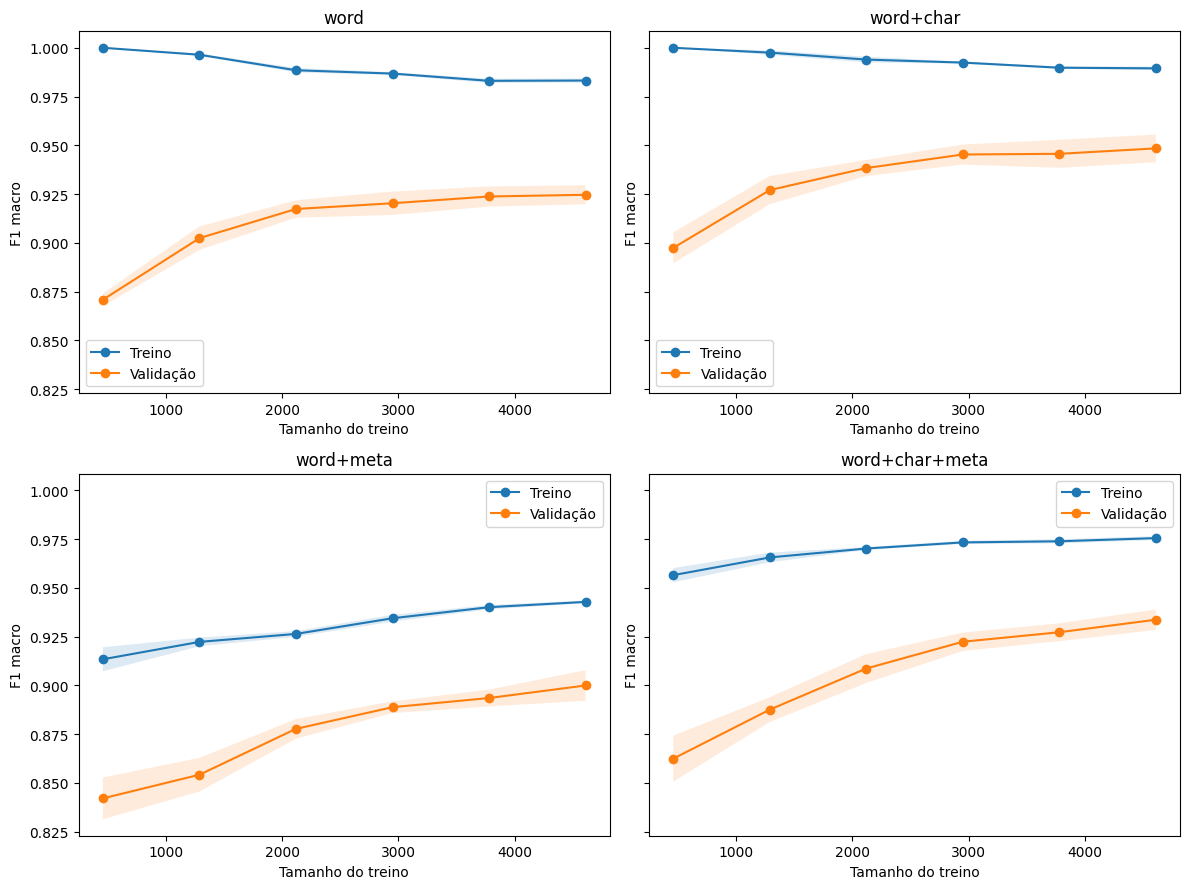
\includegraphics[width=0.8\linewidth,keepaspectratio]{entregavel-final-img/fig24.png}\\[2pt]{\small\emph{Curva de aprendizado da Regressão Logística (F1 macro de treino e validação, 5 folds; protocolo anterior). Fonte: notebook 02\_LR\_training.}}\end{center}

\paragraph{Configurações de texto}\label{configurauxe7uxf5es-de-texto}

Em word e word+char, a curva de validação praticamente estabiliza e o gap de 4 a 6 pontos não se fecha com mais dados. Isso indica variância moderada e retorno decrescente de acrescentar exemplos do mesmo corpus. O F1 de treino próximo de 1,0 é esperado em um espaço de dezenas de milhares de atributos para milhares de documentos. O padrão não sugere vazamento, já que a validação fica em torno de 0,95 e coincide com a validação cruzada.

\paragraph{Metadados}\label{metadados}

Na regressão logística, word+meta e word+char+meta ficam abaixo das versões sem metadados (−2,4 e −1,5 ponto de F1), e suas curvas ainda crescem ao final. O efeito é específico desse estimador: no LinearSVC e no Random Forest a diferença é de no máximo ≈0,4 ponto, dentro do desvio-padrão. A hipótese em investigação é a diferença de escala entre o bloco denso padronizado e o TF-IDF sob regularização L2. Essa decisão reforça a opção de não adotar os metadados como bloco principal.

\paragraph{Comparação com o LinearSVC}\label{comparauxe7uxe3o-com-o-linearsvc}

No SVM, o F1 de treino é ≈1,0 em todas as configurações. A curva de validação em função de C (config. word) atinge o máximo em C = 1 (≈0,937) e não melhora em C = 10. Reduzir C diminui o gap, mas piora a validação, e por isso os hiperparâmetros padrão foram mantidos.

\subsubsection{Dependência de convenções de redação}\label{dependuxeancia-de-convenuxe7uxf5es-de-redauxe7uxe3o}

Termos como feira, nesta, quarta e segundo concentram-se nas notícias verdadeiras (por exemplo, "nesta" aparece em 36\% das verdadeiras e 3,5\% das falsas), e lula e dilma nas falsas. Remover os marcadores temporais reduz o F1 em 0,4 a 0,9 ponto, e remover os termos políticos não altera o resultado. A análise por subgrupo (LinearSVC, config. word) revela algo que o F1 global não mostra: 27,4\% das notícias falsas com marcador temporal são classificadas como verdadeiras, contra 6,1\% nas demais (4,5×). Com treino e teste mascarados, a razão cai para 2,5× (21,1\% vs 8,3\%), o que indica que parte do efeito vem de convenções jornalísticas e parte de estilo formal mais amplo.

\pandocbounded{
\includegraphics[keepaspectratio]{entregavel-final-img/fig14.png}}

\begin{quote}
\textbf{{[}NOTA{]}} A curva de aprendizado e a análise de convenções de redação acima têm números do \textbf{protocolo anterior} (por exemplo, LR word+char com F1 de validação ≈ 0,948, enquanto o pipeline atual dá 0,9182). As conclusões qualitativas (gap que não fecha com mais dados; efeito dos marcadores temporais) são plausíveis, mas os valores precisam ser recalculados.
\end{quote}

\begin{quote}
\textbf{{[}PENDENTE{]}} Reexecutar a curva de aprendizado e a análise de subgrupo (marcadores temporais) no pipeline atual.
\end{quote}

\subsection{5.11 Modelo de produção}\label{modelo-de-produuxe7uxe3o}

\textbf{O modelo adotado para o app é o M2 + χ² (10 mil) + SVD(500)}, definido em \texttt{modelo\_olimpo.py} e exportado por \texttt{exportar\_modelo.py} (\texttt{modelVersion\ =\ "svm-spacy-chi2k10k-svd500-v1"}). O word+char completo sem spaCy (B0) é mantido como baseline de referência.

\textbf{Por que este modelo.} Na validação cruzada ele iguala o F1 do B0 (0,9295) com gap de treino--validação bem menor, e o teste interno não perde desempenho. Além disso, seus atributos de estilo podem ser calculados para qualquer texto novo, sem os metadados do corpus, e sua pontuação se decompõe exatamente em n-gramas e atributos, o que alimenta as justificativas exibidas ao jogador.

{\def\LTcaptype{none} % do not increment counter
\begin{longtable}[]{@{}
  >{\raggedright\arraybackslash}p{(\linewidth - 4\tabcolsep) * \real{0.3333}}
  >{\raggedright\arraybackslash}p{(\linewidth - 4\tabcolsep) * \real{0.3333}}
  >{\raggedright\arraybackslash}p{(\linewidth - 4\tabcolsep) * \real{0.3333}}@{}}
\toprule\noalign{}
\begin{minipage}[b]{\linewidth}\raggedright
Critério
\end{minipage} & \begin{minipage}[b]{\linewidth}\raggedright
B0 (referência)
\end{minipage} & \begin{minipage}[b]{\linewidth}\raggedright
M2 + χ² 10 mil + SVD(500) (produção)
\end{minipage} \\
\midrule\noalign{}
\endhead
\bottomrule\noalign{}
\endlastfoot
F1 CV (5 folds) & 0,9295 & 0,9295 \\
Gap treino−CV & 0,0705 & 0,042 \\
F1 teste interno & 0,9222 & 0,9243 \\
AUC externo (FakeRecogna, títulos) & 0,707 & 0,677 \\
Explicação & coeficientes por n-grama & decomposição exata por n-grama e por atributo spaCy \\
\end{longtable}
}

\textbf{Limite conhecido.} A redução do gap não melhora a generalização entre fontes: fora do Fake.br o AUC é de \textasciitilde0,68 (contra 0,707 do B0) e o F1 de \textasciitilde0,64, em títulos. O modelo deve, portanto, ser apresentado ao jogador como \textbf{indício}, e não como veredito.

\textbf{Pipeline} (entrada: texto bruto da notícia):

\begin{enumerate}
\def\labelenumi{\arabic{enumi}.}
\tightlist
\item
  \texttt{PreparadorEntrada}: aplica \texttt{normalizar} e \texttt{truncar} (idênticos ao \texttt{01\_Data\_Prep}) e extrai os 24 atributos spaCy. O modelo de linguagem é carregado sob demanda e não é gravado no arquivo exportado.
\item
  Bloco de texto: TF-IDF word+char → \texttt{SelectKBest(χ²,\ k=10\ mil)} → \texttt{TruncatedSVD(500)} → \texttt{Normalizer}.
\item
  Bloco spaCy: imputação por mediana e padronização, com peso \texttt{w\ =\ 0,03}.
\item
  \texttt{LinearSVC(C=1,\ class\_weight="balanced")} com calibração sigmoide (\texttt{CalibratedClassifierCV}, \texttt{StratifiedKFold(5)}, \texttt{ensemble=False}), que dá \texttt{P(fake)}.
\end{enumerate}

\textbf{Explicação por notícia} (\texttt{explicar}): como o bloco de texto é \texttt{z\ =\ V·x\ /\ ‖V·x‖}, o score de texto se decompõe exatamente em contribuições por n-grama selecionado, e o bloco spaCy em contribuições por atributo. \texttt{analisar} devolve o formato do contrato do backend (\texttt{classification}, \texttt{confidence}, \texttt{reasons}, \texttt{modelVersion}): \texttt{reliable} se P(fake) ≤ 0,35, \texttt{unreliable} se ≥ 0,65 e \texttt{uncertain} entre os dois. Os limiares são decisão de produto. Os motivos combinam os n-gramas de maior contribuição e frases descritivas dos atributos de estilo mais influentes.

\textbf{Exportação} (\texttt{exportar\_modelo.py}): confere que o pré-processamento reproduz o split oficial e que o pipeline não calibrado reproduz o F1 de teste do notebook 12 (0,9243, tolerância 0,002); avalia o modelo calibrado; treina o modelo final em treino+teste (7.200 notícias; \texttt{-\/-somente-treino} evita isso); salva o \texttt{.joblib} com um \texttt{.json} de metadados (versões de Python, scikit-learn, numpy, scipy, spaCy e \texttt{pt\_core\_news\_sm}, hiperparâmetros, métricas e sha256) e confere que o arquivo recarregado dá as mesmas probabilidades. O artefato fica em \texttt{modelos/} (ignorado pelo git) e só carrega se \texttt{modelo\_olimpo.py} estiver importável e as versões forem as registradas.

\section{6. Aprendizado não supervisionado}\label{aprendizado-nuxe3o-supervisionado}

A linha não supervisionada está documentada no repositório em \texttt{machine-learning/unsupervised-learning/} (branch \texttt{dev}): sete métodos de detecção de anomalias, agrupamento e aprendizado semi-supervisionado, uma comparação externa com o Jev (LLM) e, como método final de descoberta, a \textbf{mineração de padrões frequentes com FP-Growth}. As seções a seguir seguem o relatório técnico do instituto, com as referências \texttt{{[}n{]}} listadas ao final desta seção.

\subsection{6.1 Análise de classificadores não supervisionados}\label{anuxe1lise-de-classificadores-nuxe3o-supervisionados}

Analisamos os algoritmos \_K-Mean\_s, HDBSCAN, DBSCAN, One-Class SVM, LOF, FP-Growth, PU (um algoritmo semi-supervisionado), LDA e \emph{Isolation Forest.}

Enquanto os demais focam em agrupar temas ou contagem de palavras (pecando em custo computacional ou na perda do contexto semântico), o \emph{Isolation Forest} destaca-se como um excelente detector de anomalias (\emph{outliers}) focado no padrão de escrita.

\textbf{Isolation Forest}:

\begin{itemize}
\tightlist
\item
  Treinamento no padrão "normal": O modelo aprende o estilo de escrita de notícias legítimas e bem estruturadas.
\item
  Identificação de \emph{Outliers}: Notícias apelativas (com excesso de caixa alta, pontuação ou termos de urgência como \emph{"BOMBA!"}) ficam nas bordas da distribuição e são isoladas rapidamente, gerando um alto score de anomalia.
\end{itemize}

{\def\LTcaptype{none} % do not increment counter
\begin{longtable}[]{@{}
  >{\raggedright\arraybackslash}p{(\linewidth - 6\tabcolsep) * \real{0.0816}}
  >{\raggedright\arraybackslash}p{(\linewidth - 6\tabcolsep) * \real{0.2134}}
  >{\raggedright\arraybackslash}p{(\linewidth - 6\tabcolsep) * \real{0.2992}}
  >{\raggedright\arraybackslash}p{(\linewidth - 6\tabcolsep) * \real{0.4059}}@{}}
\toprule\noalign{}
\begin{minipage}[b]{\linewidth}\raggedright
\textbf{\emph{Classificador}}
\end{minipage} & \begin{minipage}[b]{\linewidth}\raggedright
\textbf{\emph{Descrição}}
\end{minipage} & \begin{minipage}[b]{\linewidth}\raggedright
\textbf{\emph{Vantagens}}
\end{minipage} & \begin{minipage}[b]{\linewidth}\raggedright
\textbf{\emph{Desvantagens}}
\end{minipage} \\
\midrule\noalign{}
\endhead
\bottomrule\noalign{}
\endlastfoot
\textbf{\emph{K-Means}} & Agrupa notícias em K clusters com base na similaridade de vetores de texto (embeddings). & · Alta velocidade de execução & \\
\end{longtable}
}

· ideal para organizar notícias já salvas do banco de dados em categorias ou "temas de fake news". \textbar{} · Exige definir o número fixo de clusters (K) previamente

· Não lida bem com ruídos ou formatos de clusters muito irregulares. \textbar{}
\textbar{} \textbf{\emph{HDBSCAN}} \textbar{} Algoritmo baseado em densidade que agrupa textos similares e identifica pontos isolados (outliers). \textbar{} · Descobre o número de clusters automaticamente

· Identifica com precisão notícias inéditas/estranhas (outliers) inseridas pelo usuário. \textbar{} · Requer maior processamento computacional e ajuste de parâmetros de densidade

· pode classificar muitos dados como ruído se descalibrado (pode dar falsos positivos) \textbar{}
\textbar{} \textbf{\emph{LDA (Latent Dirichlet Allocation)}} \textbar{} Algoritmo probabilístico de modelagem de tópicos (Topic Modeling) que extrai temas ocultos nos textos. \textbar{} · Excelente para identificar os assuntos recorrentes das notícias falsas

· Fornece contexto à LLM para gerar as perguntas socráticas. \textbar{} · Requer pré-processamento pesado de texto

· Os tópicos gerados podem ser difíceis de interpretar sem intervenção humana (Não é ideal no nosso caso, pois o humano não vai intervir nisso). \textbar{}
\textbar{} \textbf{\emph{Isolation Forest}} \textbar{} Detecta anomalias isolando pontos de dados discrepantes no espaço vetorial. \textbar{} · Perfeito para flagging de conteúdos inéditos do usuário que usam padrões textuais anômalos, sensacionalistas ou atípicos. \textbar{} · Não explica o porquê o texto é anômalo, e isso não aborda a metodologia de ensino que queremos seguir

· Necessita da LLM para analisar e desdobrar a anomalia em perguntas. \textbar{}

\subsubsection{6.1.1 Isolation Forest: funcionamento}\label{isolation-forest-funcionamento}

\textbf{Dois modos de uso.}

\begin{itemize}
\tightlist
\item
  \textbf{Detecção de novidade} (o modo usado no projeto): o modelo é treinado só com exemplos de um rótulo (aqui, notícias verdadeiras), e qualquer dado que caia fora dessa região é tratado como anomalia.
\item
  \textbf{Detecção de outliers}: o modelo é treinado com tudo misturado (por exemplo, 99\% de um rótulo e 1\% do outro) e encontra as anomalias naturalmente, por ficarem fora do centro. É útil quando os rótulos do conjunto não são conhecidos.
\end{itemize}

\textbf{Treinamento.} O algoritmo constrói árvores de isolamento. Cada árvore parte de uma amostra aleatória de registros (256 por padrão no scikit-learn). Em cada nó sorteia-se uma \emph{feature} (coluna) e, em seguida, um valor entre o menor e o maior daquela feature; os valores menores vão para a esquerda e os maiores para a direita. O processo se repete até não sobrarem pontos para separar ou até a profundidade máxima. Todo o procedimento é repetido para formar a floresta (100 árvores por padrão; os experimentos do projeto usam \texttt{n\_estimators=300}).

\textbf{Previsão.} Um dado novo percorre as árvores. Se ele é isolado por um caminho curto na maior parte delas, tem maior chance de ser anomalia; se percorre um caminho longo, tende a ser normal. O score de anomalia resume o comprimento médio desses caminhos.

{\def\LTcaptype{none} % do not increment counter
\begin{longtable}[]{@{}
  >{\raggedright\arraybackslash}p{(\linewidth - 2\tabcolsep) * \real{0.5000}}
  >{\raggedright\arraybackslash}p{(\linewidth - 2\tabcolsep) * \real{0.5000}}@{}}
\toprule\noalign{}
\begin{minipage}[b]{\linewidth}\raggedright
Vantagens
\end{minipage} & \begin{minipage}[b]{\linewidth}\raggedright
Desvantagens
\end{minipage} \\
\midrule\noalign{}
\endhead
\bottomrule\noalign{}
\endlastfoot
Tempo linear e alta velocidade: depende do tamanho das amostras, e não do tamanho do dataset & Não entende contexto \\
Pouco processamento computacional & Não explica por que o dado é anômalo \\
\end{longtable}
}

\subsubsection{6.1.2 Por que a detecção de anomalias foi a primeira abordagem}\label{por-que-a-detecuxe7uxe3o-de-anomalias-foi-a-primeira-abordagem}

A hipótese inicial foi identificar padrões linguísticos e estilísticos atípicos, frequentes em notícias falsas, que recorrem a gatilhos sensacionalistas, desvios gramaticais, pontuação ostensiva e termos apelativos para provocar reação emocional imediata. O modelo seria treinado com notícias legítimas de veículos de imprensa consolidados, o que estabelece o padrão textual esperado do jornalismo; ao receber uma notícia nova, mede o desvio em relação a esse padrão e devolve um score de anomalia.

Exemplos de pontos aberrantes esperados:

\begin{itemize}
\tightlist
\item
  \textbf{Gatilhos de urgência e alarmismo}: termos em caixa alta como "BOMBA", "URGENTE", "ATENÇÃO", "COMPARTILHE ANTES QUE APAGUE".
\item
  \textbf{Anomalias sintáticas e ortográficas}: erros gramaticais recorrentes, frases truncadas e pontuação excessiva ("!!!", "???").
\item
  \textbf{Viés emocional extremo}: vocabulário carregado de subjetividade, que apela ao medo, à raiva ou à indignação.
\end{itemize}

{\def\LTcaptype{none} % do not increment counter
\begin{longtable}[]{@{}
  >{\raggedright\arraybackslash}p{(\linewidth - 2\tabcolsep) * \real{0.5000}}
  >{\raggedright\arraybackslash}p{(\linewidth - 2\tabcolsep) * \real{0.5000}}@{}}
\toprule\noalign{}
\begin{minipage}[b]{\linewidth}\raggedright
Pontos positivos
\end{minipage} & \begin{minipage}[b]{\linewidth}\raggedright
Pontos negativos
\end{minipage} \\
\midrule\noalign{}
\endhead
\bottomrule\noalign{}
\endlastfoot
\textbf{Independência de checagem de fatos:} analisa forma e estilo, sem consultar bases em tempo real & \textbf{Não detecta mentiras bem redigidas:} notícias falsas em estilo jornalístico formal podem passar \\
\textbf{Padrões inéditos (\emph{zero-day}):} sinaliza novas narrativas assim que surgem, se houver discrepância estilística & \textbf{Falsos positivos:} opinião, sátira, crônicas e títulos legítimos propositalmente chamativos podem ser marcados \\
\textbf{Escalabilidade e agilidade:} o cálculo do score leva milissegundos e permite grande volume & \textbf{Dependência do baseline:} exige notícias legítimas atualizadas e sem vícios de escrita \\
\textbf{Sintonia com a proposta socrática e gamificada:} o score indicativo é ponto de partida para instigar a investigação, sem resposta conclusiva & \textbf{Sensibilidade à evolução da linguagem:} gírias, neologismos e mudanças de estilo podem ser lidos como desvio \\
\end{longtable}
}

\begin{quote}
\textbf{{[}NOTA{]}} O Isolation Forest foi escolhido na etapa inicial, mas a revisão crítica da seção 6.6 mostrou que suas acurácias altas (0,97) refletem a autoria do corpus e não a capacidade de detectar falsidade. Por isso o método final de descoberta passou a ser o FP-Growth (seções 6.7 e 6.8). A limitação "não explica por que o texto é anômalo" é justamente a que o projeto resolve com atributos de estilo interpretáveis e padrões do FP-Growth.
\end{quote}

\subsection{6.2 Resumo do relatório}\label{resumo-do-relatuxf3rio}

Este relatório documenta a jornada de aprendizado não supervisionado do projeto Olimpo Fake News AI. Foram examinados detectores de anomalias, métodos de agrupamento e uma linha complementar de aprendizado positivo não rotulado no corpus Fake.br. As altas acurácias de alguns detectores motivaram uma leitura inicial como classificadores, depois revista diante do viés de autoria e dos limites do conjunto. O método final de descoberta é o FP-Growth sem autoria, com controles: no treino de 4.320 notícias, ele produziu 18 conjuntos frequentes, 20 regras brutas, oito regras destacadas e dez padrões textuais. O baseline com autoria foi preservado para comparação. A avaliação posterior inclui o treino e, portanto, descreve o corpus sem medir generalização. As regras servem para formular perguntas e orientar análise humana, sem comprovar a veracidade de uma notícia.

Palavras-chave: aprendizado não supervisionado; mineração de padrões; FP-Growth; notícias falsas; viés de autoria.

\subsection{6.3 Introdução e objetivo}\label{introduuxe7uxe3o-e-objetivo}

Os tópicos abordados nesta documentação são: o comparativo de pelo menos três modelos, a indicação de quando utilizá-los, vantagens e desvantagens, a descrição de um baseline, do método final e da extração de regras {[}1{]}. Este estudo organiza essas exigências com os notebooks, scripts, manifestos e resultados desta trilha {[}2--8{]}.

O objetivo que orientou a decisão metodológica é investigar regularidades observáveis em notícias do corpus e transformá-las em perguntas verificáveis por analistas. "Notícia falsa" é o rótulo do corpus, não uma propriedade que uma medida de estilo possa demonstrar por si. Por essa razão, as pontuações de anomalia e as associações estatísticas são tratadas como sinais exploratórios.

\subsection{6.4 Dados e protocolo experimental}\label{dados-e-protocolo-experimental}

O conjunto utilizado é o Fake.br-Corpus em revisão fixa, validada por SHA-256 nos manifestos de execução. Ele contém 7.200 notícias, com 3.600 em cada classe. Na partição canônica por grupos, 4.320 registros compõem o treino, 1.440 a validação e 1.440 o teste. Os pares alinhados e duplicatas textuais normalizadas são mantidos no mesmo grupo, sem sobreposição de IDs entre partições {[}3, 4{]}.

As seis medidas de estilo são calculadas nos primeiros 300 caracteres: presença de autor, razão de tipos por tokens, densidade de links, densidade de pontuação, proporção de palavras em maiúsculas e diversidade lexical. Para descoberta temática, os notebooks usam TF-IDF de palavras e caracteres sobre textos truncados a 200 palavras. São representações diferentes e suas métricas não formam uma escala única {[}3--5{]}.

Na trilha de novidade, os algoritmos aprendem sobretudo a partir de notícias True; o limiar de alerta é o percentil 95 dos scores de True na validação. Na trilha temática, o agrupamento é exploratório. O FP-Growth usa apenas o treino canônico e não consulta o rótulo na mineração; os rótulos aparecem numa avaliação posterior dos padrões congelados {[}3, 6, 7{]}.

\subsection{6.5 Jornada dos modelos avaliados}\label{jornada-dos-modelos-avaliados}

A sequência registrada começa com variantes de detecção de anomalias, segue por agrupamento e uma linha complementar PU, e termina na mineração de padrões frequentes. Os experimentos antigos variaram texto integral, prefixo, janelas e política de autoria; permanecem como histórico e não foram misturados ao ranking canônico {[}2, 8{]}.

{\def\LTcaptype{none} % do not increment counter
\begin{longtable}[]{@{}
  >{\raggedright\arraybackslash}p{(\linewidth - 6\tabcolsep) * \real{0.0711}}
  >{\raggedright\arraybackslash}p{(\linewidth - 6\tabcolsep) * \real{0.2489}}
  >{\raggedright\arraybackslash}p{(\linewidth - 6\tabcolsep) * \real{0.2533}}
  >{\raggedright\arraybackslash}p{(\linewidth - 6\tabcolsep) * \real{0.4267}}@{}}
\toprule\noalign{}
\begin{minipage}[b]{\linewidth}\raggedright
\textbf{Método}
\end{minipage} & \begin{minipage}[b]{\linewidth}\raggedright
\textbf{Quando é indicado}
\end{minipage} & \begin{minipage}[b]{\linewidth}\raggedright
\textbf{Vantagem no projeto}
\end{minipage} & \begin{minipage}[b]{\linewidth}\raggedright
\textbf{Limitação observada}
\end{minipage} \\
\midrule\noalign{}
\endhead
\bottomrule\noalign{}
\endlastfoot
Isolation Forest & Triar desvios em atributos compactos. & Treino em True; baseline de novidade rápido e comparável. & Alerta de estilo não verifica fatos; sensível à autoria. \\
LOF & Identificar baixa densidade local em relação a vizinhos. & Bom ranking de novidade no split compartilhado. & Depende da vizinhança e da validação com rótulos. \\
One-Class SVM & Aprender fronteira de normalidade em escala adequada. & Comparação de uma hipótese geométrica distinta. & Baixo recall Fake no corte canônico. \\
K-means & Explorar grupos ou distância a centroides. & Fornece perfis temáticos e baseline de novidade. & Grupos forçados; separação temática fraca. \\
DBSCAN & Encontrar grupos densos e ruído. & Distingue cobertura, ruído e alerta. & Muitos itens sem grupo; parâmetros sensíveis. \\
HDBSCAN & Explorar densidades heterogêneas no treino. & Agrupamento sem fixar número de grupos. & Grupos extremamente enviesados para o nosso contexto, que não agregam em nada o valor dos dados. \\
PU Learning & Estudar positivos conhecidos com não rotulados. & Linha complementar para contraste. & Simulação constrói U com True conhecidos; outro protocolo. \\
\end{longtable}
}

Quadro 1 Aplicabilidade e limites dos métodos examinados. Fonte: {[}2--5, 8{]}.

O quadro distingue comparação metodológica de escolha final. HDBSCAN não fornece decisão fora da amostra no ambiente registrado; PU Learning é semissupervisionado e seu teste histórico não é diretamente comparável ao dos detectores {[}2--5{]}.

\subsubsection{6.5.1 Resultados quantitativos no protocolo canônico}\label{resultados-quantitativos-no-protocolo-canuxf4nico}

{\def\LTcaptype{none} % do not increment counter
\begin{longtable}[]{@{}
  >{\raggedright\arraybackslash}p{(\linewidth - 8\tabcolsep) * \real{0.2424}}
  >{\raggedright\arraybackslash}p{(\linewidth - 8\tabcolsep) * \real{0.1818}}
  >{\raggedright\arraybackslash}p{(\linewidth - 8\tabcolsep) * \real{0.2273}}
  >{\raggedright\arraybackslash}p{(\linewidth - 8\tabcolsep) * \real{0.1818}}
  >{\raggedright\arraybackslash}p{(\linewidth - 8\tabcolsep) * \real{0.1667}}@{}}
\toprule\noalign{}
\begin{minipage}[b]{\linewidth}\raggedright
\textbf{Método}
\end{minipage} & \begin{minipage}[b]{\linewidth}\raggedright
\textbf{Acurácia}
\end{minipage} & \begin{minipage}[b]{\linewidth}\raggedright
\textbf{Recall Fake}
\end{minipage} & \begin{minipage}[b]{\linewidth}\raggedright
\textbf{FPR True}
\end{minipage} & \begin{minipage}[b]{\linewidth}\raggedright
\textbf{ROC-AUC}
\end{minipage} \\
\midrule\noalign{}
\endhead
\bottomrule\noalign{}
\endlastfoot
Isolation Forest & 0,9729 & 0,9847 & 0,0389 & 0,9786 \\
LOF & 0,9479 & 0,9347 & 0,0389 & 0,9766 \\
One-Class SVM & 0,5563 & 0,1500 & 0,0375 & 0,8738 \\
K-means novidade & 0,5382 & 0,1111 & 0,0347 & 0,8471 \\
DBSCAN novidade & 0,9667 & 0,9847 & 0,0514 & 0,9598 \\
\end{longtable}
}

Tabela 1 Teste canônico compartilhado, com corte q95. Fonte: {[}3{]}.

No holdout temporal secundário, a acurácia do Isolation Forest cai para 0,8592 e a do DBSCAN para 0,8155; o LOF registra 0,9189. Isso reforça que o número obtido num recorte específico não basta para sustentar uma regra geral {[}3, 4{]}. Na descoberta temática canônica, K-means teve silhouette 0,0083 e HDBSCAN 0,0398 nos itens atribuídos; os valores baixos e os índices externos modestos não autorizam tratar grupos como classes de veracidade {[}3--5{]}.

\subsubsection{6.5.2 Índice de Jaccard como medida complementar}\label{uxedndice-de-jaccard-como-medida-complementar}

O grupo poderia ter usado o índice de Jaccard para quantificar a sobreposição entre conjuntos de termos ou atributos binários das notícias, ou entre conjuntos de registros cobertos por agrupamentos. Essa comparação faria sentido para os métodos de agrupamento e novidade quando representados como conjuntos; os vetores contínuos de estilo e TF-IDF exigiriam discretização ou binarização prévia. Jaccard não substituiria automaticamente as distâncias usadas nos experimentos. A lacuna de análise de sobreposição foi corrigida na etapa final: o FP-Growth calcula Jaccard entre as coberturas do antecedente e do consequente de cada regra e entre as coberturas de padrões para sinalizar redundância {[}6, 11{]}.

\subsection{6.6 Revisão crítica das acurácias}\label{revisuxe3o-cruxedtica-das-acuruxe1cias}

Houve uma interpretação intermediária equivocada: as altas acurácias dos detectores sugeriram utilizá-los como classificadores Fake/True. O experimento, porém, aprende desvio em relação ao padrão True e seleciona ou calibra componentes com a validação; o rótulo atribuído no teste é uma convenção de avaliação. Um texto atípico pode ser verdadeiro, e uma notícia falsa pode preservar o estilo de uma fonte legítima {[}3{]}.

O corpus é limitado para essa inferência. A autoria é praticamente separada por classe, as fontes e rótulos estão confundidos, a avaliação histórica consultou o teste durante o desenvolvimento e parte dos splits antigos difere do canônico. A acurácia também muda com a prevalência e o limiar. O resultado mais forte é a capacidade de reconhecer particularidades deste conjunto, não a validação factual de notícias novas {[}3, 8{]}.

O controle de autoria anterior já apontava o problema: no split por notícia, o recall anotado caía de 0,9733 com autoria para 0,6700 sem autoria; no split pareado, de 0,9750 para 0,7069. Esses números pertencem a protocolos diferentes e servem como evidência histórica de sensibilidade à feature, sem comparação direta com a Tabela 1 {[}8{]}.

\subsection{6.7 Mineração FP-Growth e extração de regras}\label{minerauxe7uxe3o-fp-growth-e-extrauxe7uxe3o-de-regras}

O FP-Growth sem autoria e com controles foi escolhido como método final de descoberta por produzir conjuntos de atributos recorrentes e regras de associação auditáveis, reduzindo a influência direta do metadado de autoria. O notebook com autoria permanece como baseline. O resultado principal é uma coleção de hipóteses sobre estilos de escrita, não uma acurácia de classificação {[}2, 6, 9{]}.

\subsubsection{6.7.1 Preparação e execução}\label{preparauxe7uxe3o-e-execuuxe7uxe3o}

Os notebooks Jupyter fp\_growth\_baseline\_com\_autoria.ipynb e fp\_growth\_principal\_sem\_autoria\_controles.ipynb validam o corpus e usam os IDs do treino canônico. O baseline inclui com\_autor e sem\_autor; o principal retira autoria da descoberta e reaproveita os mesmos limites dos itens textuais. As medidas numéricas são discretizadas pelos quantis 25\% e 75\% do treino. A densidade de links foi omitida porque ambos os quantis eram zero. O suporte mínimo é 0,08, com itemsets de até três itens; para destacar regras, os filtros exigem confidence 0,50, lift 1,05 e Jaccard 0,10 {[}6, 9{]}.

No baseline com autoria, a execução congelada encontrou 41 itemsets, 82 regras brutas, 28 elegíveis e 31 padrões consolidados. No principal sem autoria, foram 18 itemsets, 20 regras brutas, oito destacadas e dez padrões textuais. Os CSVs e manifestos preservam itens, métricas, cobertura e parâmetros; o notebook principal reúne descoberta, avaliação e controles de autoria {[}6, 9, 11{]}.

\subsubsection{6.7.2 Como ler as regras}\label{como-ler-as-regras}

Support informa a fração do treino que contém os dois lados de uma regra; confidence, a fração que contém o consequente entre as notícias com antecedente; lift compara essa proporção com a frequência geral do consequente. No experimento principal sem autoria, diversidade\_baixo → typeTokenRatio\_baixo tem support 0,172, confidence 0,684, lift 2,692 e Jaccard 0,516. O valor de Jaccard expressa a sobreposição das coberturas dos dois itens. Trata-se de coocorrência lexical, não de uma regra de falsidade {[}6, 11{]}.

A combinação punctuationDensity\_alto e typeTokenRatio\_baixo também gera duas regras direcionais. Ambas têm support 0,138 e lift 2,137, mas confidence diferente conforme o antecedente escolhido. O Apêndice C apresenta as 20 regras brutas, identifica as oito que passaram nos filtros e registra uma possível utilidade analítica para cada direção {[}11{]}.

\subsection{6.8 Avaliação externa e controles}\label{avaliauxe7uxe3o-externa-e-controles}

O notebook principal aplica os limites textuais congelados ao corpus, confere se a cobertura do treino reproduz o membership persistido e só então calcula as proporções por classe. O notebook histórico avaliou, em separado, o baseline com autoria. As avaliações abrangem as 7.200 notícias, inclusive as 4.320 usadas para descobrir padrões: são descrições do mesmo corpus, não testes independentes de generalização {[}6, 7, 9{]}.

Na avaliação dos padrões sem autoria, punctuationDensity\_alto com typeTokenRatio\_baixo aparece em 1.007 notícias, com 70,3\% Fake, perante baseline global de 50\%. Diversidade\_baixo com typeTokenRatio\_baixo aparece em 1.242 notícias, com 61,6\% Fake. Em sentido oposto, diversidade\_alto com typeTokenRatio\_alto tem 31,2\% Fake em 1.199 ocorrências. Esse lift Fake de classe difere do lift de associação calculado durante a mineração {[}6, 11{]}.

\subsubsection{6.8.1 Controle da autoria}\label{controle-da-autoria}

O controle de autoria mostra que 3.528 de 3.601 notícias sem autor são Fake, enquanto 3.527 de 3.599 com autor são Real; o Cramér V é 0,960. Dos 31 padrões do baseline, 21 contêm autoria. Portanto, um padrão com sem\_autor pode herdar quase toda a associação ao rótulo da composição do corpus. A análise principal exclui essa variável da mineração textual {[}6, 9, 11{]}.

No notebook principal, a mineração sem autoria preserva IDs e limites textuais do baseline, e as coberturas são examinadas dentro dos estratos com\_autor e sem\_autor. O padrão punctuationDensity\_alto com typeTokenRatio\_baixo tem 70,3\% Fake no agregado; no estrato com autor, tem 0,7\% perante baseline de 2,0\%; no estrato sem autor, 98,9\% perante baseline de 98,0\%. A associação agregada não pode ser atribuída isoladamente ao texto {[}6, 11{]}.

Há associações que merecem nova investigação, como punctuationDensity\_baixo com uppercaseRatio\_baixo entre notícias com autor: 32 Fake em 524 ocorrências, contra 72 Fake em 3.599 notícias desse estrato. O número de exemplos minoritários é pequeno; o resultado não estabelece causalidade, robustez por fonte ou validade fora do Fake.br {[}9{]}.

\subsection{6.9 Discussão e aplicação pelo método socrático}\label{discussuxe3o-e-aplicauxe7uxe3o-pelo-muxe9todo-socruxe1tico}

A aplicação pretendida é um roteiro de perguntas orientado por evidências. Cada padrão informa quais atributos coocorrem, em quantas notícias e com que diferença observada entre estratos. O analista então testa explicações alternativas: a ausência de autoria decorre do conteúdo ou da forma como a fonte foi coletada? A associação textual persiste quando a autoria é mantida fixa? O mesmo padrão aparece em outras fontes, temas e períodos? Notícias verdadeiras que exibem o padrão têm características contextuais semelhantes?

Esse processo é socrático porque usa as regras para questionar uma hipótese, procurar contraexemplos e delimitar o que os dados permitem concluir. A implementação atual gera padrões, coberturas e controles; a transformação desses achados em diálogo com o usuário é uma proposta de uso analítico, ainda não um módulo conversacional implementado (a interface do jogo exibe apenas cartões socráticos fixos, seção 8.4).

A prioridade seguinte de validação é aplicar critérios previamente congelados a um corpus externo com fontes e épocas distintas, registrar cobertura e efeitos por estrato e submeter os achados a revisão humana. Também convém ampliar atributos menos dependentes de metadados de publicação, mantendo a distinção entre estilo, fonte e checagem factual.

\subsection{6.10 Conclusão}\label{conclusuxe3o}

Os experimentos de anomalia e agrupamento mapearam métodos e revelaram sinais fortes, mas alta acurácia neste corpus não equivale a detecção confiável de falsidade. O FP-Growth sem autoria e com controles respondeu melhor à pergunta científica: quais combinações textuais são frequentes, quais regras direcionais elas geram e como sua leitura muda ao controlar a autoria. O Jaccard acrescentou uma medida explícita de sobreposição na etapa final. O resultado é uma base reproduzível para investigação guiada, com limites quanto a causalidade e generalização {[}6, 11{]}.

\begin{quote}
\textbf{{[}NOTA{]}} As avaliações do FP-Growth (7.200 notícias) incluem o treino de descoberta e portanto \textbf{descrevem o corpus, sem medir generalização}. As acurácias altas de Isolation Forest e DBSCAN (0,97) foram reinterpretadas no próprio relatório: os detectores aprendem desvio em relação às notícias verdadeiras, e a autoria separa as classes quase por completo. Por isso o Isolation Forest, escolhido na primeira análise (seção 6.1), deixou de ser o método final.
\end{quote}

\begin{quote}
\textbf{{[}PENDENTE{]}} O relatório aponta para arquivos no \texttt{main} (\texttt{fp\_growth\_*.ipynb}, \texttt{REGRAS\_FP\_GROWTH.md}, \texttt{history/RESULTADOS.md}). Eles estão em \texttt{dev} desde o PR \#54; conferir se o PR de \texttt{dev} para \texttt{main} já os inclui antes de manter os links. Conferido: os números do relatório batem com \texttt{history/RESULTADOS.md} e \texttt{REGRAS\_FP\_GROWTH.md}.
\end{quote}

\subsubsection{Referências do relatório não supervisionado}\label{referuxeancias-do-relatuxf3rio-nuxe3o-supervisionado}

{[}1{]} APRENDIZADO NÃO SUPERVISIONADO. Briefing em PDF, uma página. Arquivo AprendizadoNaoSupervisionado.pdf, projeto Olimpo Fake News AI.

{[}2{]} OLIMPO FAKE NEWS AI. Experimentos não supervisionados. machine-learning/unsupervised-learning/README.md. Consulta em: 30 set. 2026.

{[}3{]} OLIMPO FAKE NEWS AI. Comparação histórica dos experimentos. machine-learning/unsupervised-learning/history/RESULTADOS.md. Consulta em: 30 set. 2026.

{[}4{]} OLIMPO FAKE NEWS AI. Documentação de DBSCAN e K-means. machine-learning/unsupervised-learning/docs/modelos/dbscan.md e history/modelos/kmeans.md. Consulta em: 30 set. 2026.

{[}5{]} OLIMPO FAKE NEWS AI. Documentação de HDBSCAN e PU Learning. machine-learning/unsupervised-learning/docs/modelos/hdbscan.md e history/modelos/pu-learning.md. Consulta em: 30 set. 2026.

{[}6{]} OLIMPO FAKE NEWS AI. Notebook principal FP-Growth sem autoria e controles. machine-learning/unsupervised-learning/fp\_growth\_principal\_sem\_autoria\_controles.ipynb; run fp-growth-controls-20260929T215211Z. Consulta em: 30 set. 2026.

{[}7{]} OLIMPO FAKE NEWS AI. Notebook histórico de avaliação do FP-Growth com autoria. machine-learning/unsupervised-learning/history/mineracao-de-padroes/avaliacao\_fp\_growth\_com\_autoria.ipynb; run fp-growth-evaluation-20260929T213741Z. Consulta em: 30 set. 2026.

{[}8{]} OLIMPO FAKE NEWS AI. Modelos e experimentos anteriores. machine-learning/unsupervised-learning/history/consulta-modelos-anteriores/README.md. Consulta em: 30 set. 2026.

{[}9{]} OLIMPO FAKE NEWS AI. Notebook baseline FP-Growth com autoria. machine-learning/unsupervised-learning/fp\_growth\_baseline\_com\_autoria.ipynb; run fp-growth-20260929T212058Z. Consulta em: 30 set. 2026.

{[}10{]} INSTITUTO DE PESQUISAS ELDORADO. Logotipo institucional. Disponível em: \url{https://www.eldorado.org.br/wp-content/themes/eldorado/assets/img/logo_eldorado.svg}. Acesso em: 30 set. 2026.

{[}11{]} OLIMPO FAKE NEWS AI. Regras extraídas pelo FP-Growth e utilidade para o projeto. machine-learning/unsupervised-learning/REGRAS\_FP\_GROWTH.md. Consulta em: 30 set. 2026.

\section{7. Resultados e discussão integrada}\label{resultados-e-discussuxe3o-integrada}

\subsection{7.1 Quadro-resumo}\label{quadro-resumo}

{\def\LTcaptype{none} % do not increment counter
\begin{longtable}[]{@{}
  >{\raggedright\arraybackslash}p{(\linewidth - 6\tabcolsep) * \real{0.2500}}
  >{\raggedright\arraybackslash}p{(\linewidth - 6\tabcolsep) * \real{0.2500}}
  >{\raggedright\arraybackslash}p{(\linewidth - 6\tabcolsep) * \real{0.2500}}
  >{\raggedright\arraybackslash}p{(\linewidth - 6\tabcolsep) * \real{0.2500}}@{}}
\toprule\noalign{}
\begin{minipage}[b]{\linewidth}\raggedright
Linha de trabalho
\end{minipage} & \begin{minipage}[b]{\linewidth}\raggedright
Protocolo
\end{minipage} & \begin{minipage}[b]{\linewidth}\raggedright
Resultado principal
\end{minipage} & \begin{minipage}[b]{\linewidth}\raggedright
Como ler
\end{minipage} \\
\midrule\noalign{}
\endhead
\bottomrule\noalign{}
\endlastfoot
LinearSVC word+char, C=1 & CV 5 folds, treino do Fake.br & F1 0,9295 ± 0,0099 & referência interna atual \\
Regressão Logística word+char & CV 5 folds & F1 0,9182 ± 0,0136 (C=1) → 0,9281 (C=10) & baseline interpretável \\
Random Forest word+char & CV 5 folds, protocolo anterior & F1 0,9285 & \textbf{{[}PENDENTE{]}} reexecutar \\
Redução (χ², L1, SVD) & CV 5 folds & nenhuma supera a base & seção 5.8 \\
Kernels RBF/polinomial & CV 5 folds & sem ganho (notebook, sem CSV) & seção 5.8 \\
Teste externo FakeRecogna & treino Fake.br, títulos & F1 0,6122, AUC 0,7072, 70,7\% previsto fake & viés de domínio \\
Metadados do corpus & LR (protocolo anterior) / SVM (grid search, 3 folds) & −2,4 pt (LR); +1,4 pt (SVM) & em conflito \\
Metadados spaCy (M2) & CV 5 folds, C=1, w=0,03 & F1 0,9344 (+0,005; 5/5 folds); teste interno +0,0014; AUC externo 0,707 → 0,662 & ganho pequeno e frágil; piora a transferência \\
\textbf{M2 + χ² 10 mil + SVD(500) (modelo de produção)} & CV 5 folds & F1 0,9295, gap 0,042 (B0: 0,9295, 0,0705); AUC externo 0,677 & menos ajuste ao treino, sem ganho de generalização \\
Isolation Forest / LOF / DBSCAN & split canônico, q95 & acurácia 0,97 / 0,95 / 0,97 & descreve o corpus; reinterpretado \\
FP-Growth sem autoria & treino canônico & 18 itemsets, 8 regras destacadas, 10 padrões & hipóteses, não classificador \\
\end{longtable}
}

\subsection{7.2 O que os resultados sustentam}\label{o-que-os-resultados-sustentam}

\begin{enumerate}
\def\labelenumi{\arabic{enumi}.}
\tightlist
\item
  \textbf{Dentro do Fake.br, o problema é bem resolvido por um modelo linear simples.} O LinearSVC sobre TF-IDF word+char chega a \textasciitilde0,93 de F1 em validação cruzada; arquiteturas mais complexas (RF, kernels) e reduções de dimensionalidade não melhoram.
\item
  \textbf{Esse desempenho não se transfere.} Em títulos do FakeRecogna o F1 cai para \textasciitilde0,61, com forte viés para "fake". A distância entre os dois corpora é de domínio e de formato, e nenhuma técnica de dimensionalidade a resolveu.
\item
  \textbf{Parte do sinal é artefato da fonte.} Autoria (Cramér V 0,96), tipografia e marcadores temporais (27,4\% das falsas com marcador temporal são classificadas como verdadeiras, contra 6,1\% nas demais; protocolo anterior) explicam parte dos resultados altos. Daí a normalização, o truncamento e a decisão de tratar o FP-Growth como gerador de hipóteses. A normalização eliminou o artefato de espaços (\texttt{SPACE} de 2,93\% para 0,00\% nas falsas), mas resta um sinal de tamanho: 17\% das falsas têm menos de 100 palavras, contra \textasciitilde0\% das verdadeiras.
\item
  \textbf{Os dois métodos respondem a perguntas diferentes.} O supervisionado classifica; o não supervisionado descreve padrões de estilo que podem alimentar perguntas socráticas. Nenhum dos dois verifica fatos.
\item
  \textbf{Os metadados agregam pouco e atrapalham fora do domínio.} O bloco spaCy soma +0,005 na CV (só com peso w=0,03), não melhora o teste interno e reduz o AUC externo;
\item
  \textbf{Reduzir a dimensão não melhora a generalização.} SVD só diminui o gap por \emph{underfitting}; χ² + SVD(500) reduz o gap sem perder F1 na CV, mas piora o AUC externo (0,677 contra 0,707).
\end{enumerate}

\subsection{7.3 Limitações}\label{limitauxe7uxf5es}

\begin{itemize}
\tightlist
\item
  Um único corpus de treino, rotulado por fonte; rótulo e fonte estão confundidos.
\item
  Partição aleatória no supervisionado (pares temáticos podem cruzar treino e teste) e por grupos no não supervisionado; os dois não são comparáveis entre si.
\item
  Resultados de teste interno com a configuração já escolhida; cada configuração externa foi avaliada uma vez.
\item
  Nenhum modelo foi calibrado nem testado em notícias reais submetidas por usuários.
\end{itemize}

\section{8. MVP: plataforma Olimpo}\label{mvp-plataforma-olimpo}

\begin{quote}
\textbf{Estado}: em desenvolvimento ativo. O backend de jogo está implementado e testado; a interface já cobre o fluxo principal do jogo (seção 8.3); \textbf{o modelo de ML ainda não está integrado} e as perguntas socráticas são cartões fixos, não geradas dinamicamente.
\end{quote}

\subsection{8.1 Visão do produto}\label{visuxe3o-do-produto}

O Olimpo é uma plataforma gamificada, educativa e colaborativa para treinar o reconhecimento de notícias falsas. Em salas multiplayer ou solo, os participantes analisam manchetes sob tempo limite e votam entre \textbf{É FAKE NEWS}, \textbf{É FATO REAL} e \textbf{TENHO DÚVIDA}. Há ainda desafios autorais (um jogador cadastra uma notícia falsa convincente e ganha pontos de blefe por cada colega induzido ao erro), feedback educativo ao fim da rodada e ranking com conquistas.

\subsection{8.2 Arquitetura}\label{arquitetura}

\textbf{Stack.} Next.js 16 (App Router, Server Components e Route Handlers), React 19, TypeScript em modo estrito, Tailwind CSS v4; PostgreSQL com Drizzle ORM; Redis para publicação e assinatura de eventos; validação com Zod v4. A ingestão de notícias usa JSDOM (sem execução de scripts), \texttt{@mozilla/readability}, cliente \texttt{undici} com \emph{DNS pinning} contra DNS rebinding, \texttt{ipaddr.js} para bloquear IPs privados e a API Jina Reader como fallback.

\textbf{Camadas.} O backend segue Clean Architecture (domínio → aplicação → infraestrutura → apresentação), e o frontend segue Atomic/Feature-Sliced (\texttt{views}, \texttt{widgets}, \texttt{features}, \texttt{entities}, \texttt{components}). Fluxo de uma ação:

\begin{verbatim}
flowchart LR
  UI[Interface] --> Action[Server Action]
  Action --> Zod[Validação Zod]
  Zod --> Controller
  Controller --> UC[Caso de uso]
  UC --> RepoIF[Interface do repositório]
  RepoInf[Repositório Drizzle] -.implementa.-> RepoIF
  RepoInf --> PG[(PostgreSQL)]
  UC --> Redis[(Redis pub/sub)]
  Redis --> SSE[SSE: eventos em tempo real]
  SSE --> UI
\end{verbatim}

Regras de dependência: aplicação → domínio; infraestrutura → aplicação e domínio; domínio não importa Next.js, Drizzle nem React; o frontend nunca acessa a infraestrutura.

\begin{quote}
\textbf{{[}NOTA{]}} O \texttt{docs/codigo/arquitetura-web-app.md} e o README descrevem as camadas em \texttt{src/server/}. No código atual, cada módulo vive em \texttt{src/app/api/\textless{}módulo\textgreater{}/} (\texttt{entities}, \texttt{repositories}, \texttt{usecase}, \texttt{actions}, \texttt{tests}) e \texttt{src/server/shared} guarda apenas banco, Redis e logger. Essa organização por funcionalidade é a descrita corretamente em \texttt{docs/codigo/arquitetura.tex} (documentação de arquitetura do repositório), usada como fonte das decisões abaixo; o \texttt{architecture.md} e o README devem ser atualizados.
\end{quote}

\subsubsection{Decisões de arquitetura e trade-offs}\label{decisuxf5es-de-arquitetura-e-trade-offs}

Cada decisão segue o formato contexto, pontos positivos, pontos negativos e resolução. Fonte: \texttt{docs/codigo/arquitetura.tex} e o registro de decisões do grupo.

\paragraph{Next.js como plataforma full-stack}\label{next.js-como-plataforma-full-stack}

Escolhido pela capacidade full-stack integrada: \textbf{Server Actions} executam as mutações no servidor sem rotas de API dedicadas para cada operação, o que reduz a complexidade e a superfície de ataque, e a hospedagem gratuita para a volumetria prevista (Vercel) viabiliza o projeto.

\begin{itemize}
\tightlist
\item
  \textbf{Positivos:} desenvolvimento rápido (mesmo framework e mesma linguagem no frontend e no backend, com tipagens e funções compartilhadas e segurança de tipos de ponta a ponta); segurança (componentes e módulos \texttt{server-only} mantêm dados sensíveis e segredos no servidor, e importá-los no cliente quebra o build); sem negociação de CORS, por operar na mesma origem; React Server Components reduzem o JavaScript enviado ao navegador; hospedagem gratuita.
\item
  \textbf{Negativo:} a arquitetura \textbf{serverless não permite WebSocket nativamente}, o que afetaria o tempo real das salas e do chat em grupo.
\item
  \textbf{Resolução adotada:} tempo real por \textbf{Server-Sent Events (SSE)} com \textbf{Redis Pub/Sub} (item seguinte). Um serviço complementar de WebSocket gerenciado, como o \textbf{Ably}, foi considerado apenas como \textbf{alternativa}, caso o produto passasse a exigir comunicação bidirecional; \textbf{não foi adotado e não existe no código}.
\end{itemize}

\paragraph{Tempo real: SSE em vez de WebSocket}\label{tempo-real-sse-em-vez-de-websocket}

\begin{itemize}
\tightlist
\item
  \textbf{Unidirecionalidade:} as ações dos jogadores (entrar, votar, avançar rodada) são mutações pontuais, autenticadas e validadas, que já passam por Server Actions; o canal em tempo real só precisa levar eventos do servidor ao cliente.
\item
  \textbf{Compatibilidade com serverless e HTTP/2:} WebSocket exige servidores com conexões abertas e processos ininterruptos (ou serviços externos pagos); SSE funciona sobre HTTP comum.
\item
  \textbf{Reconexão automática:} o \texttt{EventSource} do navegador reconecta sozinho e preserva o último evento recebido, dispensando bibliotecas como Socket.io.
\item
  \textbf{Transparência em redes corporativas:} SSE trafega como HTTP na porta 443, sem o cabeçalho \texttt{Upgrade} que firewalls e proxies costumam bloquear.
\item
  \textbf{Implementação:} rota \texttt{GET\ /api/rooms/{[}pin{]}/events} com \texttt{Content-Type:\ text/event-stream}, cliente \texttt{ioredis} dedicado como assinante do canal \texttt{room:\textless{}pin\textgreater{}}, \texttt{ReadableStream} para emitir os eventos (\texttt{MEMBER\_JOINED}, \texttt{VOTE\_CAST}, \texttt{ROUND\_COMPLETED}, \texttt{MATCH\_FINISHED}) e encerramento da assinatura quando o cliente desconecta, para evitar vazamento de conexões.
\end{itemize}

\paragraph{Serverless}\label{serverless}

Custo proporcional ao uso (o tráfego de treinamentos e aulas oscila entre picos e inatividade), elasticidade e menor custo operacional. Para operar bem nesse modelo: conexões de banco e Redis reutilizadas via \texttt{globalThis}, \texttt{runtime\ =\ "nodejs"} e \texttt{dynamic\ =\ "force-dynamic"} nas rotas de SSE, e nenhum estado mutável em memória ou disco (o estado fica no JWT em cookie, no Redis ou no PostgreSQL).

\paragraph{Banco de dados: PostgreSQL no Supabase, com Redis}\label{banco-de-dados-postgresql-no-supabase-com-redis}

\begin{itemize}
\tightlist
\item
  \textbf{Contexto:} PostgreSQL oferece um motor relacional confiável, de alto rendimento e de fácil manutenção, e a hospedagem no \textbf{Supabase} atende, sem custo, ao volume de acessos previsto. O padrão de acesso de um jogo em tempo real tem dois perfis opostos, então a persistência é híbrida.
\item
  \textbf{PostgreSQL (dados duráveis e relacionais):} usuários, salas, notícias, votos e análises, com integridade referencial; a notícia extraída fica em uma coluna \textbf{JSONB} (\texttt{news\_articles.article}), que absorve a variação de metadados sem migrações destrutivas; enums nativos (\texttt{ml\_target\_type}, \texttt{vote\_option\_type} com \texttt{reliable\ /\ uncertain\ /\ unreliable}).
\item
  \textbf{Redis (dados efêmeros e de alta frequência):} busca de sala por PIN em O(1) (\texttt{room:pin:\textless{}pin\textgreater{}}), placar em \emph{sorted set} (\texttt{ZADD}/\texttt{ZREVRANGE}) e canais Pub/Sub para o SSE.
\item
  \textbf{Supabase:} operação gerenciada (sem administrar servidores nem backups), \emph{connection pooling} (Supavisor) adequado ao serverless, e console para inspeção. A conexão exige TLS (\texttt{sslmode=require}); o app usa o pooler, e as migrações usam a conexão direta.
\item
  \textbf{Sem vendor lock-in:} o Olimpo conecta-se como cliente PostgreSQL padrão, por meio do Drizzle e do \texttt{postgres.js}, e não pelo SDK do Supabase.
\item
  \textbf{Positivos:} hospedagem gratuita, conexão simples com o projeto, adequado ao uso.
\end{itemize}

\paragraph{Drizzle ORM}\label{drizzle-orm}

Camada de acesso a dados com entidades tipadas e consultas construídas no código, o que traz robustez e agiliza o desenvolvimento.

\begin{itemize}
\tightlist
\item
  \textbf{Segurança:} a manipulação direta no código com consultas parametrizadas evita SQL injection.
\item
  \textbf{Migrations:} esquemas em TypeScript geram SQL determinístico (\texttt{drizzle-kit}), versionado no Git.
\item
  \textbf{Objetos e tipagem forte:} facilita declarar entidades e reduz erros.
\end{itemize}

\paragraph{Camadas, DDD e Feature-Sliced Design}\label{camadas-ddd-e-feature-sliced-design}

\begin{quote}
\textbf{{[}NOTA{]}} O registro de decisões do grupo agrupava este item sob o título "FSD", mas o texto descreve a arquitetura em camadas do backend. São duas decisões distintas, separadas abaixo.
\end{quote}

\begin{itemize}
\tightlist
\item
  \textbf{Backend: Clean Architecture orientada a funcionalidades.} Domínio (entidades e regras) isolado de HTTP, Next.js, Drizzle e Redis; casos de uso orquestram o fluxo; repositórios são interfaces com implementações de infraestrutura; Server Actions são a porta de entrada e validam com Zod. O motivador é desacoplar as regras de domínio dos serviços de infraestrutura, de modo que um componente externo possa ser trocado (por exemplo, migrar de um SGBD relacional para NoSQL) com impacto limitado ao adaptador da camada de dados. A \textbf{injeção de dependência} permite testar os casos de uso em milissegundos com repositórios em memória.
\item
  \textbf{Frontend: Feature-Sliced Design} (\texttt{views}, \texttt{widgets}, \texttt{features}, \texttt{entities}, \texttt{components}), em que uma camada só importa de camadas abaixo dela, o que evita dependências circulares.
\item
  \textbf{Positivos:} manutenibilidade, legibilidade e possibilidade de trocar ferramentas (como o banco) sem comprometer o restante do código. \textbf{Negativos:} complexidade e maior tempo de implementação.
\end{itemize}

\paragraph{Padrões complementares}\label{padruxf5es-complementares}

\begin{itemize}
\tightlist
\item
  \textbf{Validação com Zod v4} em todas as entradas ("nunca confie na entrada do usuário").
\item
  \textbf{Autenticação própria} (e-mail e senha), com senha em hash (\texttt{bcryptjs}) e sessão por JWT em cookie \texttt{httpOnly}, que não é legível por scripts e mitiga o roubo de sessão por XSS.
\item
  \textbf{Contrato uniforme de respostas:} as actions devolvem \texttt{ActionResult\textless{}T\textgreater{}} (\texttt{\{\ success:\ true,\ data\ \}} ou \texttt{\{\ success:\ false,\ error,\ code?\ \}}), e os Route Handlers seguem o mesmo formato, com mensagens amigáveis que não expõem detalhes internos.
\item
  \textbf{OpenSpec:} especificações vivas por capacidade (\texttt{auth}, \texttt{rooms}, \texttt{news-voting}, \texttt{realtime-events}, \texttt{ai-feedback}, \texttt{gamification}), com proposta, design e tarefas para cada mudança, que mantêm humanos e agentes de IA alinhados a contratos verificáveis.
\item
  \textbf{Padrão de código} com linters, formatação e Conventional Commits (Husky e Commitlint).
\item
  \textbf{Pirâmide de testes:} testes unitários de domínio e casos de uso (Vitest), testes de Server Actions com simulação de ponta a ponta e logs estruturados, e testes E2E de interface (Playwright), todos no CI.
\end{itemize}

\paragraph{Conexão da IA com o backend}\label{conexuxe3o-da-ia-com-o-backend}

O ponto de integração é a interface de domínio \texttt{IAIAnalysisService}, injetada no caso de uso de feedback. Hoje a implementação é um mock por palavras-chave; a implementação com o modelo de produção é descrita na seção 8.5. Como o domínio só conhece o contrato, a troca não altera as regras do jogo.

\paragraph{Diagrama entidade-relacionamento}\label{diagrama-entidade-relacionamento}

Gerado a partir dos schemas do Drizzle (\texttt{src/server/shared/database/schemas/}):

\begin{verbatim}
erDiagram
  users ||--o| user_avatars : possui
  users ||--o{ rooms : "é host de"
  users ||--o{ room_members : participa
  rooms ||--o{ room_members : tem
  rooms ||--o{ room_playlist_items : "tem playlist"
  news_articles ||--o{ room_playlist_items : "compõe"
  news_articles ||--o{ news_analyses : "recebe análise"
  room_playlist_items ||--o{ news_votes : "recebe votos"
  rooms ||--o{ news_votes : registra
  users ||--o{ news_votes : emite
  news_articles ||--o{ global_challenges : "base de"
  global_challenges ||--o{ global_challenge_answers : "recebe respostas"
  users ||--o{ global_challenge_answers : responde

  users {
    text id PK
    text email UK
    text password_hash
    enum role "participant | admin"
    int xp
  }
  user_avatars {
    text user_id PK
    enum gender
    enum skin
    enum outfit
    enum headwear
  }
  rooms {
    text id PK
    varchar pin UK
    enum status "waiting | in_progress | finished"
    int round_duration_seconds
    int current_round
    int total_rounds
    text host_id FK
  }
  room_members {
    text id PK
    text room_id FK
    text user_id FK
    enum role "host | participant"
    int score
  }
  news_articles {
    text id PK
    jsonb article
    enum target_classification "reliable | uncertain | unreliable"
  }
  room_playlist_items {
    text id PK
    text room_id FK
    text article_id FK
    int round_order
  }
  news_votes {
    text id PK
    text room_id FK
    text playlist_item_id FK
    text user_id FK
    enum vote "reliable | uncertain | unreliable"
    bool is_correct
    int points_awarded
  }
  news_analyses {
    text id PK
    text article_id FK
    enum classification
    jsonb reasons
    numeric confidence
    text model_version "default mock-v1"
  }
  global_challenges {
    text id PK
    text title
    text article_id FK
    int xp_reward
    bool is_active
  }
  global_challenge_answers {
    text id PK
    text challenge_id FK
    text user_id FK
    enum answer
    bool is_correct
    int xp_awarded
  }
\end{verbatim}

Restrições de unicidade relevantes: um usuário por sala (\texttt{room\_members}), uma notícia por posição de rodada (\texttt{room\_playlist\_items}), um voto por usuário em cada item da playlist (\texttt{news\_votes}) e uma resposta por usuário em cada desafio global.

\subsection{8.3 Módulos implementados}\label{muxf3dulos-implementados}

{\def\LTcaptype{none} % do not increment counter
\begin{longtable}[]{@{}
  >{\raggedright\arraybackslash}p{(\linewidth - 2\tabcolsep) * \real{0.5000}}
  >{\raggedright\arraybackslash}p{(\linewidth - 2\tabcolsep) * \real{0.5000}}@{}}
\toprule\noalign{}
\begin{minipage}[b]{\linewidth}\raggedright
Módulo
\end{minipage} & \begin{minipage}[b]{\linewidth}\raggedright
Função
\end{minipage} \\
\midrule\noalign{}
\endhead
\bottomrule\noalign{}
\endlastfoot
\texttt{auth} & cadastro, login com JWT em cookies, resolução de sessão, avatar \\
\texttt{rooms} & ciclo de vida da sala, código PIN, playlist de notícias \\
\texttt{news-voting} & votação em três níveis, avaliação da rodada e pontuação \\
\texttt{realtime-events} & rota SSE e publicador via Redis pub/sub \\
\texttt{global-challenges} & desafios globais e respostas \\
\texttt{news/extract} & extração de título e conteúdo a partir de URL (ingestão) \\
\texttt{ai-feedback} & análise de credibilidade de cada notícia (hoje \emph{mock}) \\
\end{longtable}
}

Dados: \texttt{users}, \texttt{user\_avatars}, \texttt{rooms}, \texttt{room\_members}, \texttt{room\_playlist\_items}, \texttt{news\_articles} (com carga \texttt{jsonb}), \texttt{news\_analyses}, \texttt{news\_votes}, \texttt{global\_challenges}, \texttt{global\_challenge\_answers}. A construção seguiu o fluxo de especificação com OpenSpec (specs arquivadas e ativas por módulo) e TDD nos casos de uso.

\textbf{Qualidade.} Aproximadamente 40 arquivos de teste (Vitest) e testes ponta a ponta de ações com logs \texttt{pino}; Playwright para a interface; CI com \texttt{pnpm\ audit}, \texttt{pnpm\ check} e testes E2E; CodeQL, \emph{dependency review}, Dependabot e um revisor automatizado de PRs (Acrux).

\textbf{Interface (Next.js, Feature-Sliced Design).} As telas implementadas cobrem o fluxo principal: página inicial com os modos de jogo, criação e entrada em sala por PIN, lobby, \textbf{jogo por etapas} (checagem da notícia, aguardando o veredito com a reflexão socrática, placar da rodada e placar final), ranking, submissão de notícia ou desafio autoral, cadastro/login e extração de notícia por URL. Os eventos da sala chegam à tela por SSE.

\subsection{8.4 Estado do componente de IA}\label{estado-do-componente-de-ia}

O contrato do serviço de análise é uma interface de domínio (\texttt{IAIAnalysisService}): recebe título, conteúdo, fonte e autor e devolve \texttt{classification} (\texttt{reliable\ \textbar{}\ uncertain\ \textbar{}\ unreliable}), \texttt{confidence}, uma lista de \texttt{reasons} e \texttt{modelVersion}. A implementação atual (\texttt{MockAIAnalysisService}, \texttt{modelVersion:\ "mock-v1"}) classifica por palavras-chave (por exemplo "chocante", "bomba", "fraude" para não confiável; "universidade", "ministério", "dados oficiais" para confiável) e devolve motivos e confiança fixos por classe. A especificação já prevê o \emph{fallback} para o mock quando o serviço externo estiver indisponível.

Isso significa que o resultado das seções 5 e 6 \textbf{ainda não chega ao usuário}; a camada de domínio, porém, já isola a troca de implementação.

\textbf{Consumo pela interface.} A tela do jogo já lê o campo \texttt{analysis} (classificação, motivos e confiança) do evento de fim de rodada e o exibe, incluindo um verômetro de confiabilidade. Ou seja, o front está pronto para receber a saída do modelo real: hoje o conteúdo exibido vem do mock.

\begin{quote}
\textbf{{[}NOTA{]}} Há textos e valores \textbf{fixos} na interface, sem origem no modelo nem nos experimentos: a dica da reflexão socrática ("notícias alarmistas com títulos em maiúsculas e sem autoria clara têm 78\% mais chances de serem desinformação") e a margem de erro padrão do verômetro ("±1.8\%"). Como o modelo não foi avaliado para esses números, eles devem ser substituídos por valores medidos ou removidos antes de qualquer demonstração.
\end{quote}

\subsection{8.5 Como o MVP constrói sobre as descobertas}\label{como-o-mvp-construxf3i-sobre-as-descobertas}

O modelo de produção (seção 5.11) foi desenhado para encaixar no contrato do backend. O que falta para ele chegar ao jogador é o serviço que o expõe ao app e a troca do mock.

\begin{enumerate}
\def\labelenumi{\arabic{enumi}.}
\tightlist
\item
  \textbf{Contrato de saída alinhado.} \texttt{modelo\_olimpo.analisar} devolve exatamente o formato de \texttt{AIAnalysisResult} (\texttt{classification}, \texttt{confidence}, \texttt{reasons}, \texttt{modelVersion}), de modo que a implementação do \texttt{IAIAnalysisService} pode substituir o mock sem mudar o domínio.
\item
  \textbf{Três níveis a partir de um classificador binário.} O jogo tem \emph{reliable / uncertain / unreliable} e o modelo tem duas classes. A solução usa a probabilidade calibrada: \texttt{uncertain} entre 0,35 e 0,65, limiares que são decisão de produto.
\item
  \textbf{Entrada heterogênea.} O app recebe o texto extraído da página (\texttt{news/extract}), com tamanhos e formatos variados. O \texttt{PreparadorEntrada} aplica a mesma normalização e o mesmo truncamento em 100 palavras do treino. Risco conhecido: os atributos de estrutura de sentença saem da distribuição de treino quando o texto é curto.
\item
  \textbf{Explicação.} Os \texttt{reasons} vêm da decomposição exata do score em n-gramas e atributos de estilo, em linguagem para o jogador (por exemplo, "frases curtas", "muitas preposições"). Os padrões do FP-Growth continuam como fonte de hipóteses de estilo; a interface hoje exibe três cartões socráticos fixos, e a geração dinâmica de perguntas (por exemplo, via LLM) ainda não existe.
\item
  \textbf{Hospedagem.} O app é TypeScript e o modelo é scikit-learn/spaCy; a opção natural é um serviço Python separado exposto por HTTP, consumido pela implementação do \texttt{IAIAnalysisService}, mantendo o mock como \emph{fallback}. O \texttt{.joblib} exige o módulo \texttt{modelo\_olimpo} importável e as mesmas versões de bibliotecas, e o modelo de linguagem do spaCy é dependência de inferência.
\item
  \textbf{Registro.} Gravar o \texttt{modelVersion} em cada análise (\texttt{news\_analyses}) e medir o modelo em notícias reais coletadas pelo \texttt{news/extract}.
\end{enumerate}

\section{9. Conclusão}\label{conclusuxe3o-1}

O projeto percorreu o caminho de uma ideia de produto (avaliador socrático de notícias) para uma plataforma de jogo com backend funcional, apoiada por duas linhas de pesquisa complementares e por um modelo de produção desenhado para ser integrado.

\textbf{O que está estabelecido.} (i) Um classificador linear sobre TF-IDF word+char resolve o Fake.br com F1 ≈ 0,93 e é difícil de superar: nem reduções de dimensionalidade, nem kernels, nem modelos de árvore, nem metadados morfossintáticos trouxeram ganho relevante de F1. (ii) O regime d ≫ N e a esparsidade favorecem modelos lineares, e C=1 é o ponto ótimo do LinearSVC. (iii) A normalização do texto e o truncamento são decisões metodológicas necessárias: eliminaram o artefato de formatação (\texttt{SPACE}), embora reste um sinal de tamanho. (iv) O FP-Growth, com controle de autoria, é o método de descoberta mais útil para formular perguntas, com a ressalva de que descreve o corpus. (v) O modelo de produção, M2 + χ² + SVD(500), mantém o F1 de 0,9295 com gap de 0,042 em vez de 0,0705.

\textbf{Trade-offs assumidos.} Interpretabilidade e custo contra capacidade (linear em vez de kernel ou árvore); descoberta de padrões contra classificação (FP-Growth em vez de detector de anomalias); controle de vazamento de fonte contra desempenho aparente (normalização e truncamento reduziram o F1 interno); menor ajuste ao treino e explicação detalhada contra generalização externa (o modelo de produção tem AUC externo de 0,677, contra 0,707 do word+char completo); e escopo (jogo e backend antes da integração do modelo).

\textbf{Limites.} A generalização fora do Fake.br é fraca (F1 ≈ 0,61--0,64, AUC ≈ 0,68--0,71, em títulos), por viés de domínio que nenhuma das técnicas testadas resolveu; por isso a saída do modelo é apresentada como indício. O método socrático está implementado apenas como cartões fixos na interface, e o modelo ainda não está conectado ao \texttt{ai-feedback}.

\textbf{Próximos passos.} (1) Publicar o serviço de inferência e substituir o mock; (2) medir o modelo com notícias reais; (3) coletar um conjunto externo com texto completo de fontes e épocas distintas; (4) tornar dinâmicas as perguntas socráticas, a partir dos \texttt{reasons} e dos padrões do FP-Growth.

\section{Referências}\label{referuxeancias}

\url{https://www.ibm.com/br-pt/think/topics/logistic-regression}

\url{https://www.scirp.org/reference/referencespapers?referenceid=3092942}

\url{https://www.bbc.com/future/article/20240509-the-sift-strategy-a-four-step-method-for-spotting-misinformation}

\url{https://www.productplan.com/glossary/moscow-prioritization}

\url{https://scikit-learn.org/stable/modules/tree.html}

\url{https://github.com/GiovanniGatti/socratic-llm/tree/main}

\url{https://www.datacamp.com/pt/tutorial/introduction-to-shap-values-machine-learning-interpretability}

\url{https://huggingface.co/tasks/feature-extraction}

\url{https://www.ibm.com/think/topics/feature-extraction}

\url{https://fernandafperes.com.br/blog/interpretacao-boxplot/}

\url{https://shap.readthedocs.io/en/latest/example_notebooks/api_examples/plots/beeswarm.html}

\url{https://shap.readthedocs.io/en/latest/}

\url{https://shap.readthedocs.io/en/latest/example_notebooks/overviews/An\%20introduction\%20to\%20explainable\%20AI\%20with\%20Shapley\%20values.html}

\url{https://www.geeksforgeeks.org/data-analysis/what-is-exploratory-data-analysis/}

\url{https://www.ibm.com/br-pt/think/topics/exploratory-data-analysis}

Bibliografia:

\url{https://blog.runrun.it/metodologia-crystal/}

\href{https://www.dataphi.net/post/epic-story-e-task-como-fazer-uma-gest\%C3\%A3o-eficiente-de-escopo-de-projeto}{https://www.dataphi.net/post/epic-story-e-tarefas-como-fazer-uma-gest\%C3\%A3o-eficiente-de-escopo-de-projeto}

\url{https://www.efficientlyconnected.com/pmi-ai-project-management-standard-enterprise-governance/}

\url{https://www-datascience--pm-com.translate.goog/crisp-dm-2/?_x_tr_sl=en&_x_tr_tl=pt&_x_tr_hl=pt&_x_tr_pto=tc}

\url{https://www-6sigma-us.translate.goog/lean-six-sigma-articles/crystal-agile-methodology/?_x_tr_sl=en&_x_tr_tl=pt&_x_tr_hl=pt&_x_tr_pto=tc}

\url{https://youtu.be/G_ZETFAYxSQ?si=54Zrs0QEfuAEeGTi}

\url{https://interfacing-com.translate.goog/what-is-rasci-raci?_x_tr_sl=en&_x_tr_tl=pt&_x_tr_hl=pt&_x_tr_pto=tc}

\url{https://www.atlassian.com/br/agile/scrum/ceremonies}

\url{https://www-scrum--institute-org.translate.goog/Effort_Estimations_Planning_Poker.php?_x_tr_sl=en&_x_tr_tl=pt&_x_tr_hl=pt&_x_tr_pto=tc}

\url{https://aws.amazon.com/pt/what-is/mlops/}

\url{https://www.atlassian.com/br/work-management/project-management/raci-chart}

\url{https://www.atlassian.com/br/agile/project-management/epics-stories-themes}

\url{https://www.iso.org/home/insights-news/resources/iso-42001-explained-what-it-is.html}

\url{https://www.gov.br/mds/pt-br/acesso-a-informacao/governanca/integridade/campanhas/lgpd}

\section{Apêndices}\label{apuxeandices}

\subsection{Apêndice A --- Feature extraction e atributos derivados propostos}\label{apuxeandice-a-feature-extraction-e-atributos-derivados-propostos}

A etapa de \textbf{Feature Extraction} transforma os dados disponíveis no corpus em características mais representativas para o modelo de classificação. Embora o Fake.br Corpus já forneça métricas como número de verbos, adjetivos, advérbios, pronomes e palavras em maiúsculo, valores absolutos podem ser influenciados diretamente pelo tamanho da notícia.

Por isso, algumas dessas variáveis podem ser convertidas em \textbf{proporções e razões}, como num\_adverbios / num\_palavras ou num\_verbos\_modais / num\_verbos. Dessa forma, textos de tamanhos diferentes podem ser comparados de maneira mais adequada, permitindo representar características como intensidade de linguagem descritiva, modalização, pessoalidade e densidade lexical.

Também é possível combinar diferentes atributos para criar indicadores mais significativos. A densidade lexical, por exemplo, relaciona substantivos, verbos, adjetivos e advérbios ao total de palavras, enquanto relações como adjetivos por substantivos ou advérbios por verbos ajudam a representar aspectos específicos do estilo de escrita.

Essas características não determinam diretamente se uma notícia é verdadeira ou falsa. Elas fornecem sinais linguísticos para que o algoritmo aprenda quais padrões e combinações possuem maior poder de classificação. Posteriormente, técnicas como \textbf{SHAP} podem indicar quais desses atributos tiveram maior influência em cada resultado, permitindo gerar justificativas mais rastreáveis para a análise apresentada ao usuário.

\subsubsection{\texorpdfstring{\textbf{Atributos derivados propostos}}{Atributos derivados propostos}}\label{atributos-derivados-propostos}

{\def\LTcaptype{none} % do not increment counter
\begin{longtable}[]{@{}
  >{\raggedright\arraybackslash}p{(\linewidth - 4\tabcolsep) * \real{0.2278}}
  >{\raggedright\arraybackslash}p{(\linewidth - 4\tabcolsep) * \real{0.3671}}
  >{\raggedright\arraybackslash}p{(\linewidth - 4\tabcolsep) * \real{0.4051}}@{}}
\toprule\noalign{}
\endhead
\bottomrule\noalign{}
\endlastfoot
\textbf{\emph{Atributo}} & \textbf{\emph{Cálculo / origem}} & \textbf{\emph{O que representa}} \\
\textbf{\emph{\texttt{typeTokenRatio}}} & \texttt{num\_types\ /\ num\_tokens} & Diversidade do vocabulário em relação ao tamanho do texto \\
\textbf{\emph{\texttt{adjectiveRatio}}} & \texttt{num\_adjetivos\ /\ num\_palavras} & Intensidade relativa de linguagem descritiva ou avaliativa \\
\textbf{\emph{\texttt{adverbRatio}}} & \texttt{num\_adverbios\ /\ num\_palavras} & Frequência relativa de modificadores e intensificadores \\
\textbf{\emph{\texttt{pronounRatio}}} & \texttt{num\_pronomes\ /\ num\_palavras} & Presença relativa de referências pessoais no discurso \\
\textbf{\emph{\texttt{modalVerbRatio}}} & \texttt{num\_verbos\_modais\ /\ num\_verbos} & Grau de modalização, possibilidade, necessidade ou incerteza \\
\textbf{\emph{\texttt{imperativeSubjunctiveRatio}}} & \texttt{num\_verbos\_subj\_imp\ /\ num\_verbos} & Presença relativa de construções imperativas ou subjuntivas \\
\textbf{\emph{\texttt{personalPronounRatio}}} & \texttt{(num\_pron\_1\_2\_sing\ +\ num\_pron\_1\_plural)\ /\ num\_pronomes} & Grau de aproximação com autor, leitor ou grupo social \\
\textbf{\emph{\texttt{linkDensity}}} & \texttt{num\_links\ /\ num\_palavras} & Quantidade relativa de referências externas presentes no texto \\
\textbf{\emph{\texttt{punctuationDensity}}} & \texttt{(num\_tokens\ -\ num\_palavras)\ /\ num\_tokens} & Aproximação da densidade de elementos de pontuação \\
\end{longtable}
}

As características já fornecidas pelo próprio corpus, como pausalidade, tam\_medio\_sentenca, tam\_medio\_palavra, pct\_erros\_ortograficos, emotividade e diversidade, podem ser mantidas juntamente com esses atributos derivados. Posteriormente, análises de correlação, importância de atributos e desempenho do modelo podem determinar quais variáveis realmente agregam informação e quais apresentam redundância.

\begin{quote}
\textbf{{[}NOTA{]}} Os atributos derivados (razões como \texttt{adjectiveRatio}, \texttt{modalVerbRatio} e \texttt{typeTokenRatio}) são proposta de engenharia de atributos e não fazem parte do pipeline treinado; os atributos usados estão listados na seção 4.3.
\end{quote}

\subsection{Apêndice B --- Capturas dos resultados do FP-Growth}\label{apuxeandice-b-capturas-dos-resultados-do-fp-growth}

As figuras apresentam recortes dos resultados persistidos. O comparativo de classificação está arquivado em history/RESULTADOS.md; o FP-Growth principal é o notebook sem autoria e com controles. As capturas indicam a origem para conferir valores e protocolos.

\pandocbounded{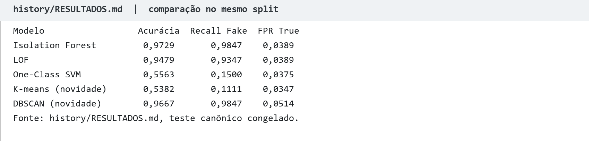
\includegraphics[keepaspectratio]{entregavel-final-img/fig15.png}}

Figura 1 Comparação resumida do teste canônico. Fonte: history/RESULTADOS.md {[}3{]}.

\pandocbounded{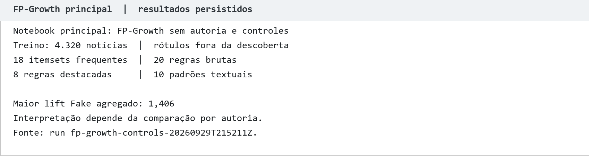
\includegraphics[keepaspectratio]{entregavel-final-img/fig16.png}}

Figura 2 Síntese do experimento principal sem autoria. Fonte: notebook principal e run de controles {[}6{]}.

\pandocbounded{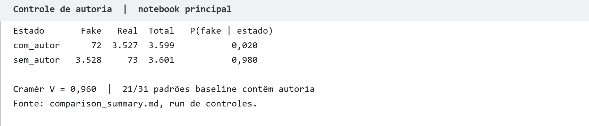
\includegraphics[keepaspectratio]{entregavel-final-img/fig17.png}}

Figura 3 Controle de autoria no corpus. Fonte: notebook principal {[}6{]}.

\subsection{Apêndice C --- Trechos do código do FP-Growth}\label{apuxeandice-c-trechos-do-cuxf3digo-do-fp-growth}

Os trechos abaixo vêm de células de código do notebook Jupyter principal. Eles documentam a extração das features, a discretização, o cálculo de Jaccard, a mineração e a conferência da cobertura antes da avaliação por classe. Linhas longas foram quebradas visualmente nas figuras.

\pandocbounded{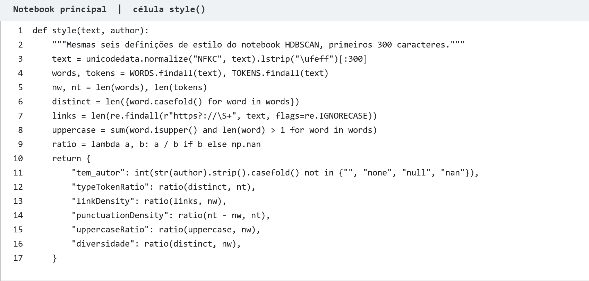
\includegraphics[keepaspectratio]{entregavel-final-img/fig18.png}}

Figura 4 Extração das medidas de estilo. Fonte: célula style() do notebook principal {[}6{]}.

\pandocbounded{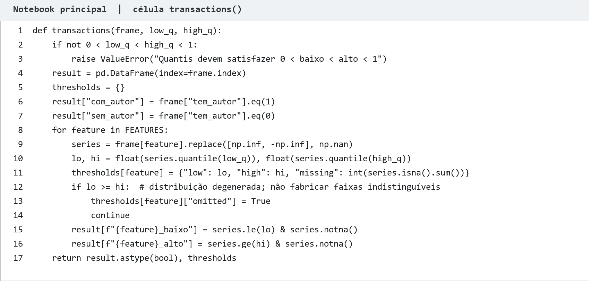
\includegraphics[keepaspectratio]{entregavel-final-img/fig19.png}}

Figura 5 Conversão de medidas em itens discretos. Fonte: célula transactions() do notebook principal {[}6{]}.

\pandocbounded{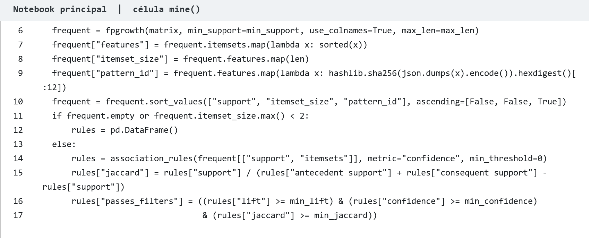
\includegraphics[keepaspectratio]{entregavel-final-img/fig20.png}}

Figura 6 Mineração, regras e Jaccard. Fonte: célula mine() do notebook principal {[}6{]}.

\pandocbounded{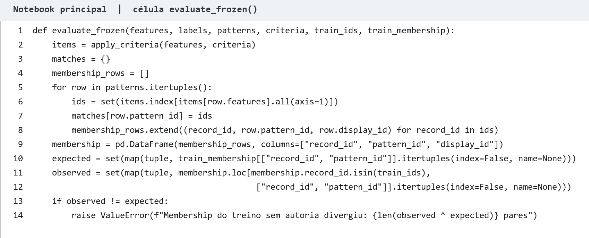
\includegraphics[keepaspectratio]{entregavel-final-img/fig21.png}}

Figura 7 Conferência da cobertura congelada. Fonte: célula evaluate\_frozen() do notebook principal {[}6{]}.

\subsection{Apêndice D --- Catálogo completo das regras extraídas}\label{apuxeandice-d-catuxe1logo-completo-das-regras-extrauxeddas}

A tabela reúne as 20 regras do experimento principal sem autoria. Oito passaram conjuntamente pelos filtros de confidence, lift e Jaccard; as outras doze permanecem no CSV bruto e são apresentadas para transparência. A direção da seta altera a confidence, mesmo quando support, lift e Jaccard são iguais. Nenhuma regra estabelece falsidade factual {[}6, 11{]}.

Legenda: TTR = razão de tipos por tokens; DIV = diversidade lexical; PONT = densidade de pontuação; MAIÚSC = proporção de maiúsculas. ↑ e ↓ indicam alto e baixo segundo os quantis do treino. S/C/L/J = support, confidence, lift de associação e Jaccard, nessa ordem.

Tabela 2 Todas as regras de associação extraídas pelo FP-Growth principal sem autoria. Fonte: {[}6, 11{]}.

{\def\LTcaptype{none} % do not increment counter
\begin{longtable}[]{@{}
  >{\raggedright\arraybackslash}p{(\linewidth - 6\tabcolsep) * \real{0.1145}}
  >{\raggedright\arraybackslash}p{(\linewidth - 6\tabcolsep) * \real{0.2214}}
  >{\raggedright\arraybackslash}p{(\linewidth - 6\tabcolsep) * \real{0.0763}}
  >{\raggedright\arraybackslash}p{(\linewidth - 6\tabcolsep) * \real{0.5878}}@{}}
\toprule\noalign{}
\begin{minipage}[b]{\linewidth}\raggedright
\textbf{Regra}
\end{minipage} & \begin{minipage}[b]{\linewidth}\raggedright
\textbf{S / C / L / J}
\end{minipage} & \begin{minipage}[b]{\linewidth}\raggedright
\textbf{Filtro}
\end{minipage} & \begin{minipage}[b]{\linewidth}\raggedright
\textbf{Como pode ajudar}
\end{minipage} \\
\midrule\noalign{}
\endhead
\bottomrule\noalign{}
\endlastfoot
DIV↓ → TTR↓ & 0,172 / 0,684 / 2,692 / 0,516 & Sim & Investigar repetição e menor variedade lexical; as duas medidas são próximas. \\
TTR↓ → DIV↓ & 0,172 / 0,677 / 2,692 / 0,516 & Sim & Testar a direção inversa e comparar a confiança da associação. \\
TTR↑ → DIV↑ & 0,166 / 0,657 / 2,557 / 0,482 & Sim & Contrastar textos com maior variedade lexical com o perfil anterior. \\
DIV↑ → TTR↑ & 0,166 / 0,645 / 2,557 / 0,482 & Sim & Testar a direção inversa e comparar a confiança da associação. \\
TTR↑ → PONT↓ & 0,138 / 0,548 / 2,163 / 0,376 & Sim & Explorar textos com menos pontuação e maior variedade de tokens. \\
PONT↓ → TTR↑ & 0,138 / 0,546 / 2,163 / 0,376 & Sim & Testar a direção inversa e comparar a confiança da associação. \\
TTR↓ → PONT↑ & 0,138 / 0,545 / 2,137 / 0,374 & Sim & Priorizar revisão humana e teste externo do maior liftFake agregado. \\
PONT↑ → TTR↓ & 0,138 / 0,543 / 2,137 / 0,374 & Sim & Testar a direção inversa e comparar a confiança da associação. \\
TTR↑ → MAIÚSC↓ & 0,119 / 0,471 / 1,080 / 0,209 & Não & Comparar variedade de tokens com menor uso de maiúsculas. \\
MAIÚSC↓ → TTR↑ & 0,119 / 0,273 / 1,080 / 0,209 & Não & Testar a direção inversa e comparar a confiança da associação. \\
PONT↓ → MAIÚSC↓ & 0,116 / 0,459 / 1,053 / 0,203 & Não & Examinar perfil de pontuação e maiúsculas, inclusive por estrato de autoria. \\
MAIÚSC↓ → PONT↓ & 0,116 / 0,267 / 1,053 / 0,203 & Não & Testar a direção inversa e comparar a confiança da associação. \\
DIV↑ → MAIÚSC↓ & 0,115 / 0,449 / 1,030 / 0,200 & Não & Investigar variedade lexical sem ênfase por maiúsculas. \\
MAIÚSC↓ → DIV↑ & 0,115 / 0,265 / 1,030 / 0,200 & Não & Testar a direção inversa e comparar a confiança da associação. \\
DIV↓ → MAIÚSC↓ & 0,105 / 0,419 / 0,961 / 0,181 & Não & Verificar repetição lexical sem maiúsculas no conjunto. \\
MAIÚSC↓ → DIV↓ & 0,105 / 0,242 / 0,961 / 0,181 & Não & Testar a direção inversa e comparar a confiança da associação. \\
TTR↓ → MAIÚSC↓ & 0,106 / 0,418 / 0,960 / 0,182 & Não & Comparar baixa variedade de tokens com menor uso de maiúsculas. \\
MAIÚSC↓ → TTR↓ & 0,106 / 0,244 / 0,960 / 0,182 & Não & Testar a direção inversa e comparar a confiança da associação. \\
PONT↑ → MAIÚSC↓ & 0,105 / 0,412 / 0,946 / 0,179 & Não & Inspecionar pontuação alta combinada a poucas maiúsculas. \\
MAIÚSC↓ → PONT↑ & 0,105 / 0,241 / 0,946 / 0,179 & Não & Testar a direção inversa e comparar a confiança da associação. \\
\end{longtable}
}

Leitura prática: as regras destacadas ajudam a formular perguntas sobre perfis de escrita. As doze regras que não passaram nos filtros servem como registro exploratório. Antes de qualquer uso preditivo, compare as associações dentro dos estratos de autoria e valide-as em notícias externas {[}11{]}.

\subsection{Apêndice E --- Planejamento (roadmap) e cumprimento}\label{apuxeandice-e-planejamento-roadmap-e-cumprimento}

O grupo definiu, na primeira semana, um roadmap de 7 semanas para a Residência em IA (Eldorado / PUC), com 6 integrantes organizados em frentes rotativas, sem papéis fixos (princípio do Crystal Clear). O quadro abaixo compara cada etapa com o que o repositório evidencia. A coluna "Entregue" só contém o que foi verificado no código e nos documentos; a coluna "Divergência" registra o que não foi cumprido ou o que a evidência desmente.

{\def\LTcaptype{none} % do not increment counter
\begin{longtable}[]{@{}
  >{\raggedright\arraybackslash}p{(\linewidth - 6\tabcolsep) * \real{0.2500}}
  >{\raggedright\arraybackslash}p{(\linewidth - 6\tabcolsep) * \real{0.2500}}
  >{\raggedright\arraybackslash}p{(\linewidth - 6\tabcolsep) * \real{0.2500}}
  >{\raggedright\arraybackslash}p{(\linewidth - 6\tabcolsep) * \real{0.2500}}@{}}
\toprule\noalign{}
\begin{minipage}[b]{\linewidth}\raggedright
Etapa
\end{minipage} & \begin{minipage}[b]{\linewidth}\raggedright
Objetivo planejado
\end{minipage} & \begin{minipage}[b]{\linewidth}\raggedright
Entregue (evidência)
\end{minipage} & \begin{minipage}[b]{\linewidth}\raggedright
Não entregue ou divergente
\end{minipage} \\
\midrule\noalign{}
\endhead
\bottomrule\noalign{}
\endlastfoot
1 & Metodologia e organização & Metodologias documentadas (seção 2): Crystal Clear, RACI, MoSCoW, Planning Poker, AIPGF, CRISP-DM, MLOps, testes e pesquisa. GitHub com PRs numerados, branches por funcionalidade, Conventional Commits e revisão automatizada & Jira, RACI e Planning Poker não deixam rastro no repositório. Os \textbf{testes metamórficos} previstos para o modelo não existem. MLOps nível 1 era a direção, mas a prática é nível 0. O DVC foi tentado (PRs \#18--\#21) e encerrado sem merge \\
2 & Arquitetura, tecnologias e dataset & Arquitetura documentada (\texttt{docs/codigo/arquitetura.tex}, OpenSpec) e tecnologias escolhidas (seção 8.2); Fake.br analisado e limpo (seção 4); variável-alvo identificada; Regressão Logística como baseline & Análise por perfil de usuário (faixa etária, região) \textbf{não foi implementada}: a tabela \texttt{users} não tem esses campos \\
3 & Estudo e experimentação de técnicas & TF-IDF e n-gramas; Regressão Logística, SVM e Random Forest comparados; várias técnicas não supervisionadas (Isolation Forest, LOF, One-Class SVM, K-means, DBSCAN, HDBSCAN, PU Learning, FP-Growth); SVD/PCA; métricas iniciais & Naive Bayes e Bag of Words aparecem só no estudo bibliográfico, sem treino. Análises por perfil de usuário não feitas \\
4 & Construção e avaliação do modelo; preparação para o backend & Pipeline de treino em Python; split controlado; accuracy, precisão, recall, F1 e matriz de confusão; várias visualizações; modelo principal documentado (seções 5 e 7); módulo de inferência isolado (\texttt{modelo\_olimpo.py}); contrato de entrada e saída (\texttt{AIAnalysisResult}) & As tabelas por modelo (LR, SVM, RF) estão no protocolo anterior; os baselines ainda não foram reexecutados no protocolo canônico comum (seção 2.10). Limitações do modelo registradas: viés de domínio, F1 ≈ 0,61 fora do Fake.br \\
5 & Motor de análise, backend e fundação do frontend & Backend com autenticação, salas, votação em três níveis (equivalente ao semáforo), SSE, desafios globais e extração de notícia com proteção contra SSRF; entradas validadas com Zod; estrutura base do frontend; a tela já consome o contrato \texttt{analysis} & \textbf{O modelo não está integrado ao fluxo de análise}: o serviço é o mock \texttt{mock-v1}, e não existe endpoint que sirva o modelo. Os sinais exibidos vêm de textos fixos do mock \\
6 & Experiência do usuário, integração e início da frente de negócio & Tela inicial, criação e entrada em sala, lobby, jogo por etapas, placares, ranking, submissão de notícia e extração por URL; semáforo de três níveis; reflexão socrática (cartões fixos) & Modo "análise livre" com a resposta do modelo: a extração por URL existe, mas não devolve análise real. Frente de negócio e pitch: \textbf{sem artefatos no repositório} \\
7 & Validação, negócio, refinamento e pitch & Documentação técnica (este documento, \texttt{docs/codigo/arquitetura.tex}, especificações OpenSpec); cerca de 40 arquivos de teste automatizados e CI com auditoria, verificação estática, E2E e CodeQL & \textbf{Sem evidência no repositório} de testes com usuários reais, feedback consolidado, evidências de impacto, proposta de valor e de negócio, pitch e plano alternativo de demonstração. Se existirem, estão fora do repositório e devem ser anexados \\
\end{longtable}
}

\textbf{Diretrizes de escopo do roadmap versus o construído.} O roadmap previa como \emph{Must Have} a classificação com score, o semáforo, a explicação por sinais, o modo desafio, a entrada manual de notícia, o modelo supervisionado, um experimento não supervisionado, as métricas e a validação com usuários. Desses, o repositório evidencia o semáforo, o modo desafio, a entrada de notícia (por URL), o modelo supervisionado, os experimentos não supervisionados e as métricas; \textbf{a classificação com score e a explicação vindas do modelo, e a validação com usuários, não estão evidenciadas}. Itens que o roadmap classificava como \emph{Could Have} (login, ranking global e funcionalidades sociais) e como \emph{Won\textquotesingle t Have} (infraestrutura avançada de multiplayer) \textbf{foram implementados}, o que mostra que a prioridade do produto passou do avaliador individual para o jogo multiplayer, antes da integração do modelo.

\end{document}
